\documentclass[a4paper,11pt, twoside]{report}

\setlength{\headheight}{13.59999pt}
\usepackage{dante}
\setlength{\parskip}{0.5em}

\fancyhead[EC,OC]{Phys 430}
\raggedbottom 

\usetikzlibrary{decorations.pathmorphing,decorations.markings,calc} % for random steps & snake
\usetikzlibrary{arrows.meta} % for arrow size
\tikzset{>=latex} % for LaTeX arrow head
\tikzstyle{radiation}=[-{Latex[length=2,width=1.5]},red!95!black!50,opacity=0.7,very thin,decorate,
                       decoration={snake,amplitude=0.7,segment length=2,post length=2}]
\begin{document}
\nocite{*}
\pagenumbering{gobble}

\setlength{\skip\footins}{0.8cm}

\newcommand\nbvspace[1][3]{\vspace*{\stretch{#1}}}
% allow some slack to avoid under/overfull boxes
\newcommand\nbstretchyspace{\spaceskip0.5em plus 0.25em minus 0.25em}
% To improve spacing on titlepages
\newcommand{\nbtitlestretch}{\spaceskip0.6em}
\pagestyle{empty}

\begin{center}
\bfseries
\nbvspace[1]
\Huge
{\nbtitlestretch\huge
PHYS 430 STATISTICAL THERMODYNAMICS}

\nbvspace[1]
\normalsize

Lecture Notes from Summer Study\\

\nbvspace[1]
\small Compiled and Written by\\
\Large DENIZ TASTAN \& MERT UNSALDI\\[0.5em]


\nbvspace[2]

%\includegraphics[width=4in]{önemli.jpg}
\nbvspace[3]
\normalsize

METU\\
\large
DEPARTMENT OF PHYSICS
\nbvspace[1]
\end{center}

\newpage

\tableofcontents

\pagenumbering{roman}
\newpage
\listoffigures
\newpage
\vspace*{\fill}
\begin{center}
    \LARGE
    This page is left blank intentionally.
\end{center}
\vspace*{\fill}
\newpage
\pagestyle{fancy}
\pagenumbering{arabic}
\chapter{The First Law of Thermodynamics}
\label{ch:Chapter1}
    Before we begin our studies on thermodynamics and statistical mechanics, we first need some fundamental definitions.
\section{Definitions}
\label{sec:1.1Definitions}
    \paragraph{System:}A collection of a large number of entities, fully or partially isolated from the rest of the universe
    \paragraph{Walls:}Boundaries between a system and the rest of the universe.
    There are three kinds of walls:
    \begin{itemize}
        \item \textbf{Adiabatic Walls:} Walls that totally isolate the system. Does not allow any passage of energy or particles.
        \item \textbf{Diathermal Walls:} Walls that only allow passage of energy.
        \item \textbf{Permeable Walls:} Walls that only allow passage of particles.
    \end{itemize}
    \paragraph{State:}Each value of a set of variables that completely describe the relevant properties of a system. 
    \begin{itemize}
        \item \textbf{Macrostates:} States with macroscopic properties that can be determined by simple measurement devices.
        \item \textbf{Microstates:} States with variables as the properties that constitute the system.
    \end{itemize}
    \begin{equation*}
        (\theta_G, V, P) \longrightarrow \text{Macrostate} \hspace{1cm} (\v{r}_1,\v{p}_1,\v{r}_2,\v{p}_2,...) \longrightarrow \text{Microstate}    
    \end{equation*}
    Here, the microstate consists of the positions and momenta of each entity that consitute the system whereas the macrostate consists of the three fundamental macroscopic properties of a system.
    \begin{itemize}
        \item \textbf{Volume} (V): The amount of space that the system occupies in the universe.
        \item \textbf{Pressure} (P): The amount of force per unit area that the particles within the system apply to the walls of the system.
        \item \textbf{Temperature} ($\theta_G$): Temperature is hard to precisely define. We leave its precise definition to later chapters. For now, let us define it as a measure of the amount of heat given to a system.
    \end{itemize}
    \paragraph{Equilibrium:}State of a system at which there is no change over time in macroscopic properties. 
    
    For a state to be a viable state of equilibrium, there are two conditions.
    \begin{enumerate}
        \item The final state that is the equilibrium must be independent of the initial state of the system.
            \begin{figure}[H]
                \centering
                \begin{tikzpicture}
    % First plot
                \begin{scope}[shift={(0,0)}]
                    \draw[->] (0,0) -- (4,0) node[right] {$V$};
                    \draw[->] (0,0) -- (0,3) node[above] {$P$};
                    \draw[dashed] (0,1.5) -- (3.5,1.5);
                    \node[left] at (0,1.5) {$P_{eq}$};
                    \draw[thick, red] (0,0.5) to[out=60,in=180] (3.5,1.5);
                    \node[below left] at (0,0.8) {$P_0$};
                \end{scope}
                
                % Second plot
                \begin{scope}[shift={(6,0)}]
                    \draw[->] (0,0) -- (4,0) node[right] {$V$};
                    \draw[->] (0,0) -- (0,3) node[above] {$P$};
                    \draw[dashed] (0,1.5) -- (3.5,1.5);
                    \node[left] at (0,1.5) {$P_{eq}$};
                    \draw[thick, red] (0,2.5)
                    to[out=-60,in=180] (3.5,1.5);
                    \node[above left] at (0,2.3) {$P_0$};
                \end{scope}
            \end{tikzpicture}
                \caption{A system at two different initial values, reaching the same equilibrium state.}
                \label{fig:equilibrium}
            \end{figure}
            
        \item The equilibrium state must be independent of the history of the system
    \end{enumerate}
    Equilibrium can be reached after given enough time in a single system as well as a collection of interacting systems. When it comes to which property stops changing over time, there are three aspects of an equilibrium state.
    \begin{enumerate}
        \item \textbf{Mechanical Equilibrium:} No change over time in the volume of the system.
        \item \textbf{Thermal Equilibrium:} No heat exchange happens between the systems.
        \item \textbf{Chemical Equilibrium:} Number of interacting particles in the system(s) do not change.
    \end{enumerate}
    For a reversible reaction \ce{A + B <=> AB},  chemical equilibrium is reached when the rate of the reaction in one direction equals the rate of the reaction in the opposite direction. At that point, reactions do not stop. However, since the rates are equal, there is no macroscopic change to the system. If all three aspects are reached, the system is said to be in a \textbf{thermodynamic equilibrium}. If two systems are in equilibrium with each other, then they are said to be \textbf{isothermal} to each other.
    \begin{law*}{Zeroth Law of Thermodynamics}
        For three interacting systems $A,B,C$; if the system $A$ is in equilibrium with the system $B$ and $B$ is in equilibrium with the system $C$, then $A$ and $C$ are also in equilibrium. 
    \end{law*}
    \noindent Now consider a reference system $A$, a gas with constant state variables $P$ and $V$ and a test system $X$. System $X$ is put in contact with $A$ for a long enough time such that they are always in equilibrium. Now, we vary the volume and the pressure of $X$ all the while keeping it isothermal to $A$. Then, we obtain a specific curve called an \textbf{isotherm.}
    \begin{figure}[H]
        \centering
        \resizebox{0.35\textwidth}{!}{%
        \begin{circuitikz}
        \tikzstyle{every node}=[font=\Large]
        \draw [line width=0.2pt, ->, >=Stealth] (11.5,18.5) -- (11.5,25);
        \draw [line width=0.2pt, ->, >=Stealth] (11.5,18.5) -- (19,18.5);
        \draw [line width=0.2pt, short, red] (12.5,24.5) .. controls (13.5,20.75) and (13.25,20) .. (18.5,19.25);
        \draw [line width=0.2pt, short, blue] (12,24.5) .. controls (12.5,21) and (12,19.5) .. (18.5,18.75);
        \draw [line width=0.2pt, short, violet] (13,24.5) .. controls (14.25,21.5) and (13.25,20.5) .. (18.5,19.75);
        \draw [line width=0.2pt, short, orange] (13.5,24.5) .. controls (14.75,21.75) and (14,21) .. (18.5,20.25);
        \node [font=\Large] at (19.25,18.5) {V};
        \node [font=\Large] at (11.5,25.5) {P};
        \node [font=\Large, blue] at (19,19) {$\theta_1$};
        \node [font=\Large, red] at (19,19.4) {$\theta_2$};
        \node [font=\Large, violet] at (19,19.8) {$\theta_3$};
        \node [font=\Large, orange] at (19,20.2) {$\theta_4$};
        \end{circuitikz}
        }%
        \caption{Isotherms for multiple systems $X_i$ that are isothermal to $A$.}
        \label{fig:isotherms}
    \end{figure}
    \noindent Repeating this with many other systems at other constant values of $P$ and $V$, we can find a relationship of the form 
    
    \begin{equation}
        \theta = F(P,V) .
        \label{eq: tempeos}
    \end{equation}
\section{Functions of State}
\label{sec:1.2Functionsofstate}
    A \textbf{function of state} is a quantity that depends on the present values of macroscopic variables. An example is that when a system is in equilibrium, the temperature is a function of state. Functions of state are described by \textbf{equations of state}. An example equation of state relating the temperature of the state to its pressure and volume is given in (\ref{eq: tempeos}). Any relevant quantity can be written as a function of state with respect to the remaining quantitites.
    \begin{equation*}
        \theta = F(P,V) \hspace{1cm} P = G(\theta,V) \hspace{1cm} V = H(\theta, P)
    \end{equation*}
    Generally, equations of states are complicated mathematical expressions. An exception to this is the equation of state for an ideal gas. 

    \noindent Isotherms of an ideal gas are given by $PV=$ constant. Then, we can choose the temperature of the ideal gas ($\theta_G$) to be proportional to $PV$. Let $R$ be the constant of proportionality per mole of a gas called the \textbf{gas constant}. Then, we obtain the equation of state (\textit{Ideal gas scale of temperature}).
    
    \begin{equation}
        \theta_G = \frac{PV}{R}
    \end{equation}
    
    For $n$ moles of particles, we obtain the familiar ideal gas equation.
    
    \begin{equation}
        PV=nR\theta_G
        \label{eq:idealgas}
    \end{equation} 
    
    A more complicated example of an equation of state is the equation for a Van der Waals gas:
    
    \begin{equation}
        \theta R = \lrp{P + \frac{a}{V^2}}(V-b).
        \label{eq:vdw}
    \end{equation}
    
\subsection{Mathematical Properties of Functions of States}
\label{subsec:1.2.1mathematicalproperties}
    Let us consider an equation of state given as $G=g(x,y)$. Then, the change in $G$ is given by
    
    \begin{equation}
        \d G = \periv{g}{x}dx + \periv{g}{y}dy .
    \end{equation}
    If we define $A \coloneqq \del_xg$ and $B \coloneqq \del_yg$, we get
    \begin{equation}
        \d G = A(x,y)dx + B(x,y)dy.
    \end{equation}
    
    Now consider the second derivatives of $g$. 
    
    \begin{equation}
        \periv{A}{y} = \periv{^2g}{y\del x} \hspace{0.5cm};\hspace{0.5cm} \periv{B}{x} = \periv{^2g}{x\del y}
    \end{equation}
    
    For continuous and differentiable functions, differentiation operator commutes. Then, the order of differentiation does not matter and we get
    
    \begin{equation}
        \periv{A}{y} = \periv{B}{x}.
        \label{eq:analytic}
    \end{equation}
    
    Any function $g(x,y)$ that satisfies (\ref{eq:analytic}) is called an \textbf{analytic function}. $G$ is a function of state only if $g(x,y)$ is analytic. 
    
    Now, let us obtain $g(x,y)$ given a differential $\d G$. Defining a vector $\d\v{G}$ from a vector $\v{G}(x,y)$ where
    
    \begin{equation}
        \v{G} = A\bas{x} + B\bas{y},
    \end{equation}
    we get
    \begin{equation}
        \d\v{G} = \v{G}\cdot \d\v{r}.
    \end{equation}
    If we consider a line integral around a closed contour $\gamma$
    \begin{equation}
        \oint_\gamma \v{G}\cdot\d\v{r},
    \end{equation}
    by Stokes' theorem, we get
    \begin{equation}
        \oint_\gamma \v{G}\cdot\d\v{r} = \iint_S\lrp{\nabla\times\v{G}}\cdot\d\v{S}.
    \end{equation}
    Calculating the curl, $x$ and $y$ components vanish and we get
    \begin{equation}
        \nabla\times\v{G} = (\del_xB-\del_yA)\bas{k}.
    \end{equation}
    
    If we assume that $G$ is a function of state, these two derivatives are equal to each other. Thus, we get
    
    \begin{equation}
        \oint_\gamma \v{G}\cdot\d\v{r} = 0.
        \label{eq:closecontour}
    \end{equation}
    
    For a better analysis, let us break down the integral into two paths. 
        \begin{figure}[H]
            \centering
            \resizebox{0.4\textwidth}{!}{%
            \begin{circuitikz}
            \tikzstyle{every node}=[font=\large]
            \draw [line width = 1.2pt, -, postaction={decorate}, decoration={markings, mark=at position 0.4 with {\arrow{>}}}] (12.75,21) .. controls (20.5,26.25) and (16.75,19.75) .. (23.25,21.5);
            \draw [line width=1.2pt, -, postaction={decorate}, decoration={markings, mark=at position 0.3 with {\arrow{<}}}] (12.75,21) .. controls (14.75,16.75) and (19.75,19.25) .. (23.25,21.5);
            \draw [line width=2pt, ->, >=Stealth, blue] (11,15.75) -- (22.75,21.25);
            \draw [line width=2pt, ->, >=Stealth, blue] (11,15.75) -- (12.75,20.75);
            \draw [ fill={rgb,255:red,0; green,0; blue,0} , line width=0.2pt ] (23.2,21.5) circle (0.1cm);
            \draw [ fill={rgb,255:red,0; green,0; blue,0} , line width=0.2pt ] (12.75,21) circle (0.1cm);
            \node [font=\huge, blue] at (12,20.25) {$\v{r}_1$};
            \node [font=\huge, blue] at (23,20.5) {$\v{r}_2$};
            \node [font=\huge] at (12,22) {$\gamma$};
            \node [font=\huge] at (14,18.5) {$\gamma_1$};
            \node [font=\huge] at (17,24) {$\gamma_2$};
            \end{circuitikz}}
            \caption{\label{fig:path} A closed contour $\gamma$ is broken down into two paths $\gamma_1$ and $\gamma_2$}
        \end{figure}
    \noindent Then, the integral in (\ref{eq:closecontour}) is written as
        
        \begin{equation}
             \oint_\gamma \v{G}\cdot\d\v{r} = \lrp{\int_{\v{r}_1}^{\v{r}_2}\v{G}\cdot\d\v{r}}_{\gamma_1} + \lrp{\int_{\v{r}_2}^{\v{r}_1}\v{G}\cdot\d\v{r}}_{\gamma_2} = 0.
        \end{equation}
        \begin{equation}
           \Rightarrow     \lrp{\int_{\v{r}_1}^{\v{r}_2}\v{G}\cdot\d\v{r}}_{\gamma_1} =  \lrp{\int_{\v{r}_1}^{\v{r}_2}\v{G}\cdot\d\v{r}}_{\gamma_2}
        \end{equation}     
        
    Therefore, the line integral of $\v{G}$ is independent of the path taken. This results in the integral
    
    \begin{equation}
        g(x,y) = \int_{\v{r}_1}^{\v{r}}\v{G}\cdot\d\v{r}
    \end{equation}
    
    having a well-defined and unique value for any arbitrary $\v{r} = x\bas{x}+y\bas{y}$. Now, consider a small change $\d G$. 
    \begin{equation}
        \d G = g(x+\d x, y+\d y) - g(x,y)= \int_{\v{r}_1}^{\v{r}+\d\v{r}}\v{G}\cdot\d\v{r}-\int_{\v{r}_1}^\v{r}\v{G}\cdot\d\v{r} = \int_\v{r}^{\v{r}+\d\v{r}}\v{G}\cdot\d\v{r}
    \end{equation}
    Since this integral is independent of the path between $\v{r}$ and $\v{r}+\d\v{r}$, $\d G$ is called an \textbf{exact differential}. If $A$ and $B$ do not satisfy (\ref{eq:analytic}), then $\d G \longmapsto \dbar G$ is an \textbf{inexact differential}
\newpage

\section{Internal Energy}
\label{sec:1.3internalenergy}
    Now, let us make two more definitions:
    \begin{itemize}
        \item \textbf{Process:} A change in the state of the system that takes it from an initial configuration to a final configuration.
        \item \textbf{Initial Energy:} The energy (kinetic and potential) contained within the system.
    \end{itemize}
    
    The initial energy is always defined with respect to a reference point.
    
    \begin{equation}
        U = U_0 + \Delta U
    \end{equation}
    
    The state of an isolated system, i.e., the internal is changed by either doing work on the system or heating the system. 
    Assume that the state of the system is changed by doing work. The amount of work done to cause an equal change is independent of the means by which the work is performed. Moreover if several processes occur, the final equilibrium state depends only on the total amount of work done and not on the order in which it was done. \\
    \\
    \noindent Here, we give the First Law of Thermodynamics.
    \begin{law*}{The First Law of Thermodynamics}
        In a closed system, the change in the internal energy of the system is equal to the sum of the work done and the heat applied to the system by the surroundings. When heat is taken into account energy is always conserved.
        
        \begin{equation}
            \Delta U = W+Q
        \end{equation}
    \end{law*}
    \paragraph{Note!} In chemistry, the work done is taken to be a negative quantity such that $-W > 0$. Then, the first law is written as $\Delta U = Q - W$. As we will show later, work is not an exact differential. Therefore, from the First Law, the heat is also an inexact differential. 
    
    There are two ways to change the state of a system.

    \subsection{Reversible and Irreversible Processes}
        
        Imagine a gas in an adiabatic container with a movable piston of area $A$ and a mass $m$ on the piston as given in Figure (\ref{fig:reversible}). After the system reaches equilibrium, an infinitesimal mass $\delta m$ is added. 
        
        \begin{minipage}{0.5\textwidth}
        \begin{figure}[H]
            \centering
            \resizebox{0.3\textwidth}{!}{%
            \begin{circuitikz}
            \tikzstyle{every node}=[font=\LARGE]
            \draw [line width=2pt, short] (4.25,11.25) -- (4.25,7);
            \draw [line width=2pt, short] (4.25,7) -- (8.5,7);
            \draw [line width=2pt, short] (8.5,7) -- (8.5,11.25);
            \draw [line width=2pt, short] (4.25,11.25) -- (5,11.25);
            \draw [line width=2pt, short] (5,11.25) -- (5,7.75);
            \draw [line width=2pt, short] (5,7.75) -- (7.75,7.75);
            \draw [line width=2pt, short] (7.75,7.75) -- (7.75,11.25);
            \draw [line width=2pt, short] (7.75,11.25) -- (8.5,11.25);
            \draw [line width=1pt, short] (5,10.5) -- (7.75,10.5);
            \draw [line width=1pt, short] (5,10) -- (7.75,10);
            \draw [, line width=1pt ] (5.5,11.5) rectangle (6.5,10.5);
            \node at (5.75,9.25) [circ, blue] {};
            \node at (5.5,8.25) [circ, blue] {};
            \node at (6.5,9.25) [circ, blue] {};
            \node at (7.25,9.5) [circ, blue] {};
            \node at (5.75,9.75) [circ, blue] {};
            \node at (7.25,8.75) [circ, blue] {};
            \node at (6,8.75) [circ, blue] {};
            \node at (7.25,8.25) [circ, blue] {};
            \node [font=\Large] at (6,11) {m};
            \node [font=\Large] at (7.1,10.90) {A};
            \node [font= \Large] at (6.4, 8) {P,V};
            \end{circuitikz}
            }%

            \caption{An adiabatic system at equilibrium.}
            \label{fig:reversible}
        \end{figure}
        \end{minipage}
        \hfill
        \begin{minipage}{0.5\textwidth}
            \begin{equation}
                P_0 \longmapsto P = P_0 +\delta P
            \end{equation}
            \begin{equation}
                V_0 \longmapsto V = V_0 +\delta V
            \end{equation}
            \vfill
        \end{minipage}\\
        
        After the additional mass is added, enough time passes so that the system is at an equilibrium again. At that point the mass is removed again and system is left to reach the equilibrium. Then, in total, we have
        
        \begin{equation*}
            (P_0,V_0,\theta_G^0) \xlongrightarrow[]{+\delta m} (P,V,\theta_G) \xlongrightarrow[]{-\delta m} (P_0,V_0,\theta_G^0).
        \end{equation*}
        
        The question to ask here is that how much work is done on the system by the added mass? Since the mass does gravitational work on the system, we have
        
        \begin{equation}
            \dbar W = (m+\delta m)gdz.
        \end{equation}
        
        If we divide and multiply the right-hand side by ($-A$), we get
        
        \begin{equation}
            \dbar W = -\frac{m+\delta m}{A}g(-Adz).
        \end{equation}
        
        We can now define an volume element $dV = \v{A}\cdot d\v{z} = (a\bas{k})\cdot(-dz\bas{k})=-Adz$. Substituting this into (1.3.6),
        
        \begin{equation}
            \dbar W = -\frac{m+\delta m}{A}gdV = -\frac{mg}{A}dV - \frac{\delta mg}{A}dV = -(P+\delta P)dV.
        \end{equation}
        
        Neglecting the infinitesimal term, we obtain the expression for the work done.
        
        \begin{equation}
            \dbar W = -PdV
        \end{equation}
        
        If this equality holds, then the process is said to be a \textbf{reversible process}. Therefore, the First Law for a reversible process becomes $dU = \dbar Q_{\text{rev}} -PdV$. However, since the system is insulated, $\dbar Q_\text{rev}=0$.
        
        \begin{equation}
            dU = -PdV \Rightarrow \Delta W = -\int_{V_1}^{V_2}PdV
            \label{eq:work}
        \end{equation}
        
        Now consider two point $(P_1, V_1)$ and $(P_2, V_2)$ and choose two paths connecting the points. Since the work done is the integral of the area under each path, two different paths will give two different values for the work done. Therefore, the work is not a path-independent quantity:
        
        \begin{equation}
            \oint dW \neq 0.
        \end{equation}
        
        Because of this, work is not a function of state. By the First Law, this also forces the heat to not be a function of state.
        
        For an ideal gas, (\ref{eq:work}) gives
        
        \begin{equation}
            \Delta W = -nR\theta_G\int_{V_1}^{V_2}\frac{dV}{V} = -nR\theta_G\ln\lrp{\frac{V_2}{V_1}}.
        \end{equation}
      
      In general, however, work is larger than $-PdV$. Suppose that we put a mass $\Delta m$ on the system given in Figure (\ref{fig:reversible}) that is comparable to $m$. Then, the second term in (1.3.7) cannot be neglected anymore and we get $\dbar W \geq -PdV$. Such processes are called \textbf{irreversible processes}. A common example for irreversible processes are the sudden processes.
       
        Assume that in Figure (\ref{fig:reversible}), we suddenly push the piston such that $V_0\mapsto V_0/2$ rather than adding a mass. Then the system goes into a state $(P_1, V_0/2, \theta_1)$. Since we give energy to the system, $\theta_0<\theta_1$ and since $\Delta U = \Delta W$, $P_1\neq2P_0$. After the equilibrium is reached, we suddenly pull the piston. Here, at the instant the piston is pulled, the gas molecules have not diffused to fill the space and therefore piston does not have contact with the gas molecules. Then $\Delta\theta=0\Rightarrow\Delta U = 0$. The temperature does not change and we know that $\theta_1>\theta_0$. This means that $P_2\neq P_0$. Therefore, after doing the opposite of the action, we have not reached the same state as before and as such, sudden processes are irreversible.
    \subsection{Heat Capacities}
    \label{subsec:1.3.1Heatcapacities}
        \paragraph{Heat Capacity ($C$):} A measure of how much heat is required for a given change in temperature.
        
        Since heat is not a function of state, the path must be specified. Then, we have two possibilities:
        \begin{enumerate}
            \item \textbf{Constant Volume:} From First Law, $dU = \dbar Q + \dbar W$.
            
            \begin{equation}
                \Rightarrow C_V = \periv{Q}{\theta} = \periv{U}{\theta}-\periv{W}{\theta}
            \end{equation}
            
            For reversible processes $\dbar W = -pdV$ and since volume is constant, $dV=0$.
            
            \begin{equation}
                \therefore C_V = \periv{U}{\theta}
            \end{equation}
            
            \item \textbf{Constant Pressure:} 
            
            \begin{equation}
                C_P = \periv{Q}{\theta} = \periv{U}{\theta}-\periv{W}{\theta} = C_V+P\periv{V}{\theta}
            \end{equation}
        \end{enumerate}
        In the second case, energy goes to change both the temperature and the volume. Thus, we can see that $C_P > C_V$. For an ideal gas; $PV = nR\theta$ and $\boxed{U=\frac{3}{2}nR\theta}$\footnote{This formula will be discussed later.}. 
        \begin{equation}
            \boxed{C_V = \periv{U}{\theta} = \frac{3nR}{2} \hspace{0.5cm},\hspace{0.5cm} C_P = C_V + P\periv{V}{\theta}=\frac{3}{2}nR + P\frac{nR}{P} = \frac{5}{2}nR}
        \end{equation}
        
        \begin{problem}{Derive pressure as a function of volume in a reversible, \\adiabatic process for an ideal gas.}
            kSince the process is adiabatic, $dU = \dbar Q + \dbar W = -PdV$.
            On the other hand, $dU = \periv{U}{\theta}d\theta = C_Vd\theta$. Combining these two, we get $d\theta = - \frac{P}{C_V}dV$. From ideal gas equation,
            \begin{equation}
                PV = nR\theta \Rightarrow PdV + VdP = nRd\theta = -\frac{nRP}{C_V}dV.
            \end{equation}
            \begin{equation}
                PdV\lrp{1+\frac{nR}{C_V}} + VdP = 0
            \end{equation}
            The term in the parenthesis can be written as $(C_V+nR)/C_V = C_P/C_V$. Defining $\gamma = C_P/C_V$, we get
            \begin{equation}
                P\gamma dV + VdP = 0.
            \end{equation}
            Dividing both sides by $PV$ and integrating yields,
            \begin{equation}
                \ln P + \gamma\ln V = C' \Rightarrow PV^\gamma = C.
            \end{equation}
            Then we obtain,
            \begin{equation}
                \boxed{P = CV^{-\gamma}}
            \end{equation}
        \end{problem}
    In a more general case, the equilibrium state is characterised by $U$ and a general set of variables $\v{X}$. Then the First Law is $dU = \dbar Q + \v{f}\cdot d\v{X}$ where $\v{f}$ is a vector of generalised coordinates and $d\v{x}$ corresponds to a set of conjugate variables. We will see that we can write the heat using the temperature as a variable as $\dbar Q = TdS$. Then, $U$ becomes a function $U=U(S,\v{X})$. Similarly, we can incorporate $T$ into $\v{f}$. Note that $\v{f}$ are intersive (size-independent) variables while $\v{x}$ are extensive variables. 

    Depending on the experimental conditions, it may be necessary to switch between these two sets. This is done by defining a function $f=f(x_1,...,x_n)$. Then, $df = \sum_{i=1}^nu_idx_i$ where $u_i$ is the partial derivative of $f$ with respect to $x_i$. At this point, we can define another function that switches the focus from $x_i$ to $u_i$ for some of the variables.
        \begin{equation}
            g \coloneqq f-\sum_{i=r+1}^nu_ix_i \Rightarrow dg = df-\sum_{i=r+1}^n(u_idx_i+x_idu_i)
        \end{equation}
        Substituting (1.3.21),
        \begin{equation}
            dg = \sum_{i=1}^n u_idx_i - \sum_{i=r+1}^n(u_idx_i+x_idu_i) = \sum_{i=1}^ru_idx_i-\sum_{i=r+1}^nx_idu_i.
        \end{equation}
        Thus, we have obtained $g$ as $g=g(x_1,...x_r;u_{r+1},...,u_n)$. This function that connects $x_i$ to $u_i$ defined by the function $f$ is called the \textbf{Legendre Transformation} of $f$.
\section{Thermodynamic Functions}
\label{sec:1.4thermodynamicfunctions}
        The equilibrium state is a stationary point in the "energy" function. The particular function to be minimised depends on the experimental conditions. In general, we have three such functions.
        \begin{enumerate}
            \item \textbf{Helmholtz Free Energy (F)}: $S\longleftrightarrow \theta$, $F=U-\theta S$.
            \begin{equation}
                dF = dU -Sd\theta-\theta dS = \theta dS -PdV -Sd\theta-\theta dS=-(PdV+Sd\theta)
            \end{equation}
            \item \textbf{Gibbs Free Energy (G)}: $S\longleftrightarrow \theta$, $P\longleftrightarrow-V$, $G=U-\theta S+PV$.
            \begin{equation}
                dG = \theta dS-PdV-\theta dS-Sd\theta+PdV+VdP = VdP-Sd\theta
            \end{equation}
            \item \textbf{Enthalpy (H):} $P\longleftrightarrow-V$, $H=U+PV$.
            \begin{equation}
                dH = \theta dS - PdV + PdV + VdP = \theta dS+VdP
            \end{equation}
        \end{enumerate}
        Looking at the derivative of enthalpy with respect to temperature,
        \begin{equation}
            \periv{H}{\theta} = \periv{U}{\theta} + P\periv{V}{\theta} = \periv{Q}{\theta}-P\periv{V}{\theta}+P\periv{V}{\theta}=\periv{Q}{\theta}
        \end{equation}
        \begin{equation}
            \therefore C_P = \periv{H}{\theta}
        \end{equation}
    \section{Exercises}
        \begin{eocproblem*}{1.2 from Bowley \& Sanchez}
            By writing the internal energy as a function of state $U(\theta,V)$, show that 
            \begin{equation}
                \dbar Q = \lrp{\periv{U}{\theta}}_Vd\theta+\lrb{\lrp{\periv{U}{V}}_\theta+P}dV.
            \end{equation}
        \end{eocproblem*}
        \noindent We know that we have, 
        \begin{equation}
            dU = \dbar Q + \dbar W = \dbar Q -PdV.
        \end{equation}
        Moreover since $U=U(\theta,V)$,
        \begin{equation}
            dU = \periv{U}{\theta}d\theta + \periv{U}{V}dV.
        \end{equation}
        Then,
        \begin{equation}
            \boxed{\dbar Q = \periv{U}{\theta}d\theta + \lrp{\periv{U}{V}+P}dV}.
        \end{equation}
\newpage
        \begin{eocproblem*}{1.4 from Bowley \& Sanchez}
            The equations listed below are not exact differentials. Find for each equation an integrating factor, $g(y,z) = y^\alpha z^\beta$, where $\alpha$ and $\beta$ can be any number, that will turn it into an exact differential.\\
            (a) $dx = 12z^2dy+18yzdz$\\
            (b) $dx = 2e^{-z}dy-ye^{-z}dz$
        \end{eocproblem*}
        \textbf{A]} 
        \begin{equation}
            dx = 12z^2dy + 18yzdz \Rightarrow  dx' = 12z^2y^\alpha z^\beta dy + 18yzy^\alpha z^\beta dz
        \end{equation}
        \begin{equation}
            \periv{x}{y} = 12y^\alpha z^{2+\beta} \hspace{0.5cm} \& \hspace{0.5cm} \periv{x}{z} = 18y^{\alpha+1}z^{\beta+1}
        \end{equation}
        \begin{equation}
            \begin{cases}
                \periv{^2x}{z\del y} = 12(2+\beta)y^\alpha z^{\beta+1} \\ 
                \periv{^2x}{y\del z} = 18(\alpha + 1)y^\alpha z^{\beta+1}
            \end{cases} \Rightarrow 12(2+\beta)y^\alpha z^{\beta+1} = 18(\alpha+1)y^\alpha z^{\beta+1}
        \end{equation}
        \begin{equation}
            \Rightarrow 12(2+\beta) = 18(\alpha+1) \Rightarrow 12\beta = 18\alpha -6 \Rightarrow 2\beta = 3\alpha-1
        \end{equation}
        \begin{equation}
            \boxed{\therefore \beta = \frac{1}{2}(3\alpha-1)}
        \end{equation}
        \textbf{B]}
        \begin{equation}
            dx = 2e^{-z}dy - ye^{-z}dz \Rightarrow dx' = 2e^{-z}y^\alpha z^\beta dy - ye^{-z}y^\alpha z^\beta dz
        \end{equation}
        \begin{equation}
            \begin{cases}
                \periv{^2x}{z\del y} = -2e^{-z}y^\alpha z^\beta +2\beta e^{-z}y^\alpha z^\beta \\ 
                \periv{^2x}{y\del z} = -e^{-z}(\alpha+1)y^\alpha z^\beta
            \end{cases} 
        \end{equation}
        \begin{equation}
            \Rightarrow -2e^{-z}y^\alpha z^\beta +2\beta e^{-z}y^\alpha z^\beta = -e^{-z}(\alpha+1)y^\alpha z^\beta \Rightarrow 2(\beta-1) = - (\alpha + 1)
        \end{equation}
        \begin{equation}
            \Rightarrow 2\beta-2 = -\alpha-1 \Rightarrow 2\beta = 1-\alpha
        \end{equation}
        \begin{equation}
            \boxed{\therefore \beta = \frac{1}{2}(1-\alpha)}
        \end{equation}
        
        \begin{eocproblem*}{1.6}
            For an ideal gas, $PV=nR\theta$ where $n$ is the number of moles. Show that the heat transferred in an infinitesimal quasistatic process of an ideal gas can be written as
            \begin{equation}
                \dbar Q = \frac{C_V}{nR}VdP+\frac{C_P}{nR}PdV.
            \end{equation}
        \end{eocproblem*}
        Let us take the differential of the ideal gas law: $VdP + PdV = nRd\theta$
        For such a process, we have two cases: Constant volume ($dV=0$) and constant pressure $(dP=0)$.
            \begin{equation}
                VdP = nRd\theta \Rightarrow \frac{V}{nR}dP = d\theta
            \end{equation}
            \begin{equation}
                PdV = nRd\theta \Rightarrow \frac{P}{nR}dV = d\theta
            \end{equation}
        Considering the enthalpy.
        \begin{equation}
            H = U + PV \Rightarrow dU + PdV + VdP
        \end{equation}
        Now we have everything we need to solve the question. Let us begin with $dU = \dbar Q + \dbar W = \dbar Q - PdV $.
        \begin{equation}
            \Rightarrow \dbar Q = dU + PdV = \lrp{\periv{U}{\theta}}_Vd\theta + \lrp{\periv{U}{\theta}}_Pd\theta + PdV
        \end{equation}
        Recall the heat capacity at constant volume. Since $dV=0$, $\dbar W=0$ and
        \begin{equation}
            C_V = \lrp{\periv{Q_\text{rev}}{\theta}}_V = \lrp{\periv{U}{\theta}}_V.
        \end{equation}
        Substituting this into (1.5.19),
        \begin{equation}
            \dbar Q = C_Vd\theta + \lrp{\periv{U}{\theta}}_Pd\theta + PdV.
        \end{equation}
        Since we know that the first term has constant volume, we can substitute (1.5.16) for $d\theta$. Similarly, we can multiply and divide the last term by $d\theta$. Then, we have
        \begin{equation}
            \dbar Q = \frac{VC_V}{nR}dP + \lrp{\periv{U}{\theta}}_Pd\theta + P\deriv{V}{\theta}d\theta = \frac{VC_V}{nR}dP + \lrb{\lrp{\periv{U}{\theta}}_P + P\deriv{V}{\theta}}d\theta.
        \end{equation}
        Now, the last term has constant pressure. Thus, we can substitute the expression in (1.5.17). Moreover, note that the term in the paranthesis is the heat capacity at constant pressure. Then, 
        \begin{equation}
            \boxed{\dbar Q = \frac{C_V}{nR}VdP + \frac{C_P}{nR}PdV}.
        \end{equation}

        \begin{eocproblem*}{1.7 from Bowley \& Sanchez}
            Suppose the pressure of a gas equals $\alpha V^{-\gamma}$ for an adiabatic change. Obtain an expression for the work done in a reversible adiabatic change between volumes $V_1$ and $V_2$. 
        \end{eocproblem*}
        
        \begin{equation}
            \dbar W = -PdV + \dbar Q = -\alpha V^{-\gamma}dV
        \end{equation}
        \begin{equation}
            W = -\alpha\int_{V_1}^{V_2}V^{-\gamma}dV = -\frac{\alpha}{1-\gamma}V^{1-\gamma}\bigg|_{V_1}^{V_2}
        \end{equation}
        \begin{equation}
            \boxed{\therefore W = -\frac{\alpha}{1-\gamma}\lrp{V_2^{1-\gamma}-V_1^{1-\gamma}}}
        \end{equation}
\newpage
        \begin{eocproblem*}{1.9 from Bowley \& Sanchez}
            A system consists of a gas inside a cylinder. Inside the cylinder there is a 10$\si{\ohm}$ resistor connected to an electrical circuit through which a current can pass. A mass of $0.1\si{\kilo\gram}$ is placed on the piston which drops by $0.2\si{m}$ and comes to rest. A current of $0.1\si{A}$ is passed through the $10\si{\ohm}$ resistor for $2\si{s}$. What is the change in the internal energy of the system when it has reached equilibrium?
        \end{eocproblem*}
        \begin{equation}
            \Delta U = W = W_m+W_R
        \end{equation}
        \begin{equation}
            W_m = mgh = 0.2\times 0.1 \times 10 = 0.2\si{J}
        \end{equation}
        \begin{equation}
            W_R = Pt = I^2Rt = (0.1)^2\times10\times2=0.1\times2=0.2\si{J}
        \end{equation}
        \begin{equation}
            \boxed{\therefore \Delta U = 0.4\si{J}}
        \end{equation}
        
        \begin{eocproblem*}{1.10 from Bowley \& Sanchez}
            Consider $n$ moles of an ideal monatomic gas at initial pressure $P_1$ and volume $V_1$ which expands reversibly to a new volume $V_2 = V_1(1+\varepsilon)$ with $\varepsilon$ small. Use a $P-V$ diagram to establish in which of the following conditions the system does most and least work; check your answer by calculating the work done by the system in each of these circumstances. [Hint: work to second order in $\varepsilon$]\\
            (a) isobaric (the system expands at constant pressure);\\
            (b) isothermal (the system expands at constant temperature); \\
            (c) adiabatic (no heat enters when the system expands).
        \end{eocproblem*}
        \noindent Starting this problem, we plot the $P-V$ diagrams for each of the cases. First condition has constant pressure throughout. Thus, we have a straight line. In second condition, since the temperature is constant and we have an ideal gas, we can use $PV=nR\theta=$ constant. Then, the relation between the pressure and the volume is $P\propto V^{-1}$. Finally, for the last case recall the result we obtained in (1.3.15) and (1.3.20). For an reversible adiabatic process, we have $P\propto V^{-\gamma}$ and for an ideal gas, $\gamma = 5/3$. Then, the plots are: \\
        \begin{figure}[H]
            \centering
            \begin{tikzpicture}[scale=0.6]
                \begin{axis}[
                    axis lines = middle,
                    xlabel = {$V$},
                    ylabel = {$P$},
                    xmin=0, xmax=3,
                    ymin=0, ymax=2,
                    xtick={1,2},
                    xticklabels={$V_1$, $V_2$},
                    ytick={1},
                    yticklabels={$P_1$},
                    xlabel style={below right},
                    ylabel style={above left}
                ]
                % Isobaric process
                \addplot [
                    domain=1:2,
                    samples=2,
                    color=green,
                    thick,
                    dashed
                ] {1};
                \addplot [
                    domain=0:1,
                    samples=2,
                    color=black,
                    thick,
                    dashed
                ] {1};
                % Isothermal process
                \addplot [
                    domain=1:2,
                    samples=100,
                    color=blue,
                    thick,
                    dotted
                ] {1/x};
            
                % Adiabatic process
                \addplot [
                    domain=1:2,
                    samples=100,
                    color=red,
                    thick,
                    dashdotted
                ] {1/(x^1.4)};
                 
                % Labels
                \node at (axis cs:1.5,1.05) [anchor=south] {isobaric};
                \node at (axis cs:2,0.6) [anchor=west] {isothermal};
                \node at (axis cs:2,0.35) [anchor=west] {adiabatic};
                \end{axis}
            \end{tikzpicture}
            \caption{$P-V$ plots for the three cases}
            \label{fig:prob110}
        \end{figure}
        \noindent Since the work is the are under each of these curves between $V_1$ and $V_2$, we have 
        \begin{equation}
            W_\text{adiabatic} < W_\text{isothermal} < W_\text{isobaric}.
        \end{equation}
        Now, we obtain this result by calculating each value of work by integration. 
        For the first case, since pressure is constant,
        \begin{equation}
            W_\text{isobaric} = P_1(V_2-V_1) = P_1V_1(1+\varepsilon-1) = P_1V_1\varepsilon.
        \end{equation}
        For the second, we use the ideal gas law.
        \begin{equation}
            PV=nR\theta \Rightarrow P = \frac{nR\theta}{V}
        \end{equation}
        \begin{equation}
            W_\text{isothermal} = -\int P dV = -\int_{V_1}^{V_2}\frac{nR\theta}{V}dV = -nR\theta\ln\lrp{\frac{V_2}{V_1}} = -nR\theta\ln\lrp{1+\varepsilon}
        \end{equation}
        Since we want the magnitude, let us take this work as positive. Since $nR\theta$ is constant, we can write it as $P_1V_1$. So that we have a common factor in all three cases. Moreover, let us expand the natural logarithm by its Taylor series up to second order in $\varepsilon$.
        \begin{equation}
            W_\text{isothermal} = P_1V_1\lrp{\varepsilon-\frac{\varepsilon^2}{2}}
        \end{equation}
        Now, we look at the last case. We know that for adiabatic processes, $PV^\gamma = k$ where $k$ is a constant. 
        \begin{equation}
            W_\text{adiabatic} = -k\int_{V_1}^{V_2}V^{-\gamma}dV=-\frac{k}{1-\gamma}\lrp{V_2^{1-\gamma}-V_1^{1-\gamma}}
        \end{equation}
        \begin{equation}
            W_\text{adiabatic} = -\frac{kV_1^{1-\gamma}}{1-\gamma}\lrp{(1+\varepsilon)^{1-\gamma}-1}
        \end{equation}
        Now, we use the binomial expansion to $(1+\varepsilon)$ term. 
        \begin{equation}
            (1+\varepsilon)^{1-\gamma} = 1+(1-\gamma)\varepsilon+\frac{1}{2}(1-\gamma)(-\gamma)\varepsilon^2
        \end{equation}
        Then, 
        \begin{equation}
            W_\text{adiabatic} = -\frac{kV_1^{1-\gamma}}{1-\gamma}\lrb{(1-\gamma)\varepsilon-\frac{\gamma}{2}(1-\gamma)\varepsilon^2}=-kV_1^{1-\gamma}\lrp{\varepsilon-\frac{\gamma}{2}\varepsilon^2}.
        \end{equation}
        Since $k$ is a constant, $P_1V_1^{\gamma}=k$. We again take the magnitude of the work. Then,
        \begin{equation}
            W_\text{adiabatic} = P_1V_1^\gamma V_1^{1-\gamma}\lrp{\varepsilon-\frac{\gamma}{2}\varepsilon^2} = P_1V_1\lrp{\varepsilon-\frac{\gamma}{2}\varepsilon^2}.
        \end{equation}
        Since $\gamma>1$, $W_\text{isothermal}>W_\text{adiabatic}$. And clearly, $W_\text{isobaric}>W_\text{isothermal}$. Thus, we indeed showed that
        \begin{equation}
            W_\text{adiabatic}<W_\text{isothermal}<W_\text{isobaric}.
        \end{equation}
\chapter{Entropy}
\label{ch:Chapter2}
    \begin{tcolorbox}
        \paragraph{A digression:} In Problem 1.4, we came across the concept of an integrating factor. Recall that an inexact differential $\dbar z$ can be turned into an exact differential by multiplying with an integrating factor $n(x,y)$. 
        \begin{equation}
            \dbar z \longmapsto dz = n(x,y)\dbar z
        \end{equation}
    \end{tcolorbox}
    
    Now a question is that whether such an integrating factor can be written for $\dbar Q$. To answer this question, let us start from the differential of heat for an ideal gas. Here, we have two equations we can look at: Ideal gas law and the internal energy for an ideal gas.
    \begin{equation}
        PV=nR\theta \hspace{1cm} U=\frac{3}{2}nR\theta
    \end{equation}
    Using the subscript "rev" for a reversible process, we can write 
    \begin{equation}
        \dbar Q_\text{rev} = dU + PdV = \frac{3}{2}nRd\theta + \frac{nR\theta}{V}dV
        \label{eq:exactheat}
    \end{equation}  
    The second term in (\ref{eq:exactheat}) could be easily integrated had the $\theta$ term not been there. Then, let us divide the equation by $\theta$ to get
    \begin{equation}
        \frac{\dbar Q}{\theta} = \frac{3}{2}nR\frac{d\theta}{\theta} + \frac{nR}{V}dV
    \end{equation}
    Integrating this equation between an initial state $(i)$ and a final state $(f)$ of the gas, we see that LHS is now an exact differential. 
    \begin{equation}
        \int_i^f\frac{\dbar Q}{\theta} = \frac{3}{2}nR\ln\lrp{\frac{\theta_f}{\theta_i}}+nR\ln\lrp{\frac{V_f}{V_i}}
        \label{eq:exactidealheat}
    \end{equation}
    Thus, while $\dbar Q$ was an inexact differential, $\frac{\dbar Q}{\theta}$ is an exact one. Then, we can say that $1/\theta$ is an integrating factor. Let us now define a new function $S$ whose differential $dS$ is the new exact heat differential.
    \begin{equation}
        dS = \frac{\dbar Q}{\theta} \Rightarrow \int_i^f\frac{\dbar Q}{\theta} = \int_i^fdS = S_f-S_i
        \label{eq:entropy}
    \end{equation}
\newpage
    This new function is called the $\textbf{entropy}$ of the system. Combining $(\ref{eq:exactidealheat})$ and $(\ref{eq:entropy})$ we get the entropy of an ideal gas system.
    \begin{equation}
        \Delta S = \frac{3}{2}nR\ln\lrp{\frac{\theta_f}{\theta_i}}+nR\ln\lrp{\frac{V_f}{V_i}}
        \label{eq:entropydefn}
    \end{equation}
    Although we have obtained this integrating factor and defined the entropy using the ideal gas law, this expression is valid for all types of systems. Proof of this fact will not be given in this course. \\
    \\
    Consider two gases initially in two different states $(P_1,V_1,\theta_1)$ and $(P_2,V_2,\theta_2)$ separated by an adiabatic wall. When the wall is removed and enough time passes, the two gases will mix and go into a new equilibrium state $(P,V,\theta)$. This is a \textbf{spontaneous process}: A process that occurs naturally, without any outside influence. As expected, the gases will not suddenly separate and go back to their initial, non-equilibrium states. Spontaneous processes occur in a way that the entropy of the system increase. This is expressed in the Second Law of Thermodynamics.
    \begin{law*}{The Second Law of Thermodynamics}
        The sum of the entropies of the initially isolated systems is less than or equal to the total entropy of the final combination. Equaility occurs just when the two original have all their respective intensive variables equal; then the final system also has the same values.
    \end{law*}
    A corollary of the Second Law is given below.
    \begin{lawcorollary*}{Corollary 1}
        Heat spontaneously flows from a hot to a cold body.
    \end{lawcorollary*}
    The second law has many consequences and is one of the must fundamental aspects of our universe. Let us look at some of them.
    \section{The Carnot Cycle}
    \label{sec:2.1Carnotcylce}
        Imagine a spontaneous heat flow from a hot body to a cold body. If one of these bodies is much larger than the other, then the temperature of that body will not change in equal amounts to the cold one. 
        \paragraph{Reservoir / Heat Bath:} A large body whose temperature does not change upon addition of a finite temperature.
\newpage
        This flow of heat from a hot body to a cold body can be used to produce work. This work is substanially increased if the two bodies undergoing heat exchange are both reservoirs and that they do not reach an equilibrium state easily. As demonstrated in Figure (\ref{fig:engine}) this occurs as:
        \begin{itemize}
            \item $Q_H$ leaves the hot reservoir.
            \item Some system converts some of the heat into work.
            \item $Q_C$ flows from the system into the cold reservoir.
        \end{itemize}
        \begin{figure}[H]
            \centering
            \resizebox{0.6\textwidth}{!}{
            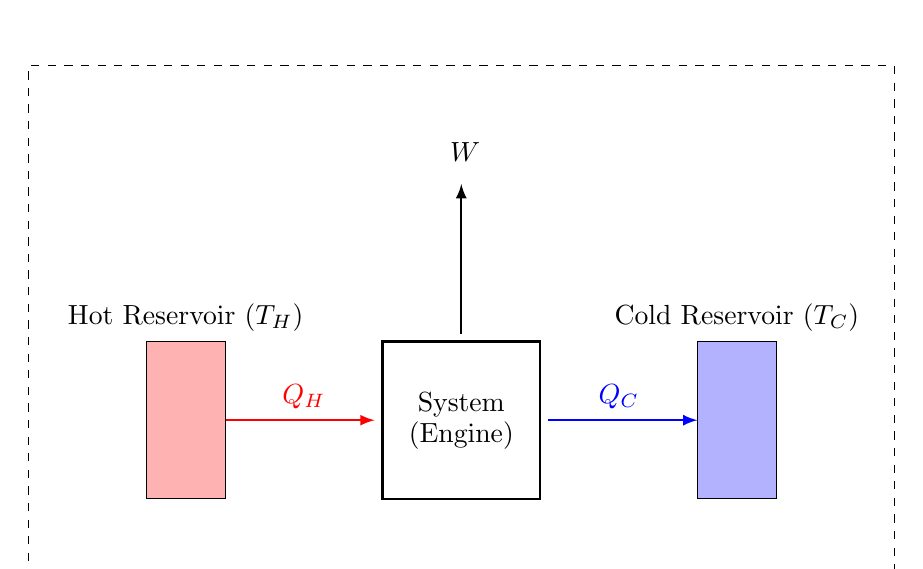
\begin{tikzpicture}
                % Hot Reservoir
                \fill[red!30] (-4, 1) rectangle (-3, -1);
                \node at (-3.5, 1.3) {Hot Reservoir ($T_H$)};
                
                % Cold Reservoir
                \fill[blue!30] (3, 1) rectangle (4, -1);
                \node at (3.5, 1.3) {Cold Reservoir ($T_C$)};
                
                % Working Substance (inside a box)
                \draw[thick] (-1, -1) rectangle (1, 1);
                \node at (0, 0.2) {System};
                \node at (0, -0.2) {(Engine)};
                %bi dk bekle olmuştu mq olum buna direkt system yazak bi de rezrvuarların contourlarını düz çizgi yapsana dashed olmasın yaptım bi de carnot cycle'ı sil genel bi engine olsun bu
                % Heat flow from Hot Reservoir to Working Substance
                \draw[->, thick, red] (-3, 0) -- (-1.1, 0);
                \node[red] at (-2, 0.3) {$Q_H$};
                
                % Heat flow from Working Substance to Cold Reservoir
                \draw[->, thick, blue] (1.1, 0) -- (3, 0);
                \node[blue] at (2, 0.3) {$Q_C$};
                
                % Work done by the engine
                \draw[->, thick, black] (0, 1.1) -- (0, 3);
                \node[black] at (0.05, 3.4) {$W$};
            
                % Carnot Cycle Box
                \draw[dashed] (-5.5, -2) rectangle (5.5, 4.5);
                \node at (-3.5, 3) {};
                % Hot resevoir contour
                \draw[-] (-4, -1) rectangle (-3, 1);
                \node at (-3.5, 3) {};
                % Hot resevoir contour
                \draw[-] (3, -1) rectangle (4, 1);
                \node at (-3.5, 3) {};
            \end{tikzpicture}
            }
            \caption{Diagram of a basic heat engine.}
            \label{fig:engine}
        \end{figure}
        
        \paragraph{Heat Engine: } A system that operates between a hot and a cold reservoir, producing work. \\
        In an ideal heat engine, the work produced equals the difference between the heat transferred between the engine and the reservoirs. Thus, all of the heat difference is converted to work.
        \begin{equation}
            W = Q_H - Q_C
        \end{equation}
        The \textbf{efficiency} of such an engine is defined as
        \begin{equation}
            \eta = \frac{W}{Q_H}
        \end{equation}
        By definition, we see that the efficiency can never be $100\%$. Such a case would require $Q_C=0$. A question is then: What is the highest efficiency engine one can define? For this, an engine must operate in a cyclical manner so that it is reusable. Such an engine is called a \textbf{Carnot engine}: A cyclical engine that is made up of four reversible processes. 
        \begin{enumerate}
            \item Isothermal expansion. A heat input of $Q_1$ is applied. Since the process is isothermal, internal energy is constant. $P\propto V^{-1}$.
            \item Adiabatic expansion. $\Delta Q=0$. $P\propto V^{-\gamma}$.
            \item Isothermal compression. Heat $Q_2$ is taken out of the system. The internal energy is constant. $P\propto V^{-1}$.
            \item Adiabatic compression. $\Delta Q = 0$. $P\propto V^{-\gamma}$. 
        \end{enumerate}
        This cycle is called the \textbf{Carnot cycle}. Since this engine is reversible, it can be run backwards. 

        \begin{figure}[t]
            \centering
                \begin{tikzpicture}
                [
                % Corner style
                    corner/.style={ 
                        circle,
                        fill,   
                        inner sep=1pt},
                % Line with Arrow style
                    arrowline/.style={
                        thick,
                        postaction = decorate,
                        decoration = {markings,
                            mark = at position .6 with \arrow{latex}
                        }
                    }]
                % Draw axis with labels
                \draw [latex-latex] (0,5)  |- (8,0) 
                    node [pos=.95,below] {V}
                    node [pos=0.07,left] {P};
                 
                % Cycle corners
                \node[corner,
                    label = {left:$1$}] (1) at (1,4.5){} ;
                 
                \node[corner,
                    label = {right:$2$}] (2) at (4,3.5){} ;
                 
                \node[corner,
                    label = {right:$3$}] (3) at (5,1){} ;
                 
                \node[corner,
                    label = {below left:$4$}] (4) at (1.5,2){} ;
                 
                % Curved lines
                \draw [name path = A, arrowline,blue!70] (1) to [bend right = 15] 
                    node [pos = .4] {} (2);
                 
                \draw [name path = B, arrowline,red!70 ] (2) to [bend right = 15] 
                    node [pos = .4] {}(3);
                 
                \draw [name path = C, arrowline,blue!70] (3) to [bend left  = 15] 
                    node [pos = .4] {} (4);
                 
                \draw [name path = D, arrowline,red!70 ] (4) to [bend left  = 15] 
                    node [pos = .4] {} (1);

                % Heat input and output
                \draw[->, thick, black] (3.2, 4.47) -- (3.2, 3.67
                );
                \node[black] at (3.5, 4.4) {$Q_1$};
                \draw[->, thick, black] (3.2, 1) -- (3.2, 0.3);
                \node[black] at (2.9, 0.3) {$Q_2$};
                % Work
                \fill[blue!20,opacity=0.7] (1) to [bend right=15] (2) to [bend right=15] (3) to [bend left=15] (4) to [bend left=15] (1);
                \node[black] at (2.7,2.7) {$W$};
                \end{tikzpicture}
            \caption{P-V plot of the Carnot engine.}
            \label{fig:carnotcycle}
        \end{figure}
        $P-V$ diagram of these processes are given in Fig (\ref{fig:carnotcycle}). The area between these four curves gives the work obtained from the engine. Moreover, since the overall change in the internal energy is zero, $W=\Delta Q = Q_1-Q_2$. Therefore, the efficiency is 
        \begin{equation}
            \eta = \frac{W}{Q_1}= 1-\frac{Q_2}{Q_1} < 1.
        \end{equation}
        This shows that an engine with $100\%$ efficiency is not possible. Other than being the simplest engine, Carnot engine has one more important property.
        \begin{theorem}{Carnot Theorem}
            bThe most efficient engine is the Carnot engine.
        \end{theorem}
        Now let us prove this theorem. There are two parts to this proof: \\
        \begin{wrapfigure}{l}{0.5\textwidth}
            \centering
            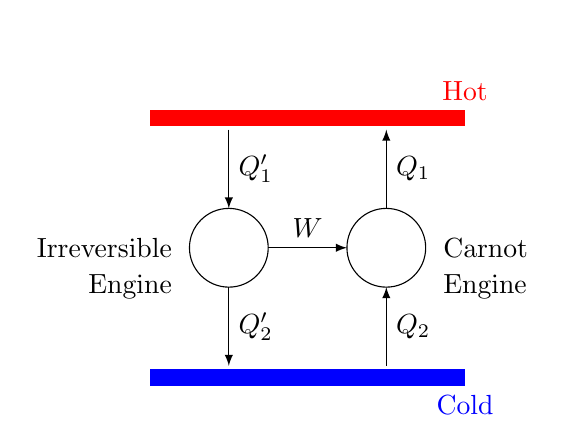
\begin{tikzpicture}
                % Draw the hot and cold reservoirs
                \draw[line width=6pt, red] (-2,1.65) -- (2,1.65) node[above] {\textcolor{red}{Hot}};
                \draw[line width=6pt, blue] (-2,-1.65) -- (2,-1.65) node[below] {\textcolor{blue}{Cold}};
            
                % Draw the circles for the Carnot engine and evaporative engine

                \draw (-1,0) circle (0.5) node[left=0.6cm] {Irreversible};
                \draw (-1,-0.5)  node[left=0.6cm] {Engine};
                \draw (1,0) circle (0.5) node[right=0.6cm] {Carnot};
                \draw (1,-0.5)  node[right=0.6cm] {Engine};                
            
                % Draw the arrows and labels
                \draw[->] (-1,1.5) -- (-1,0.5) node[midway,right] {$Q_1'$};
                \draw[<-] (1,1.5) -- (1,0.5) node[midway,right] {$Q_1$};
                \draw[->] (-1,-0.5) -- (-1,-1.5) node[midway,right] {$Q_2'$};
                \draw[<-] (1,-0.5) -- (1,-1.5) node[midway,right] {$Q_2$};
                \draw[->] (-0.5,0) -- (0.5,0) node[midway,above] {$W$};
            
                % Add labels for heat flow directions
                \node at (0,2.2) {};
                \node at (0,-2.2) {};
             \end{tikzpicture}
             \caption{An irreversible engine and a Carnot engine sharing the same reservoirs.}
             \label{fig:irrevcarnot}
        \end{wrapfigure}
        First we have to prove that no irreversible engine is more efficient than the Carnot engine, given that both engines run between the same reservoirs. As seen in Figure (\ref{fig:irrevcarnot}), the irreversible engine is used to run the Carnot engine backwards. Then,
        \begin{equation}
            \eta_I = \frac{W}{Q_1'} \hspace{0.6cm} \eta_C = \frac{W}{Q_1}.
        \end{equation}
        Note that for the efficiency of the Carnot engine, we have used $Q_1$ despite the engine running from the cold reservoir to the hot one. When calculating the efficiency, what matters is the heat corresponding to the hot reservoir, no matter the direction. Let us first assume that the efficiency of the irreversible engine is larger than the Carnot engine. 
        \begin{equation}
            \eta_I > \eta_C \Rightarrow \frac{W}{Q_1'} > \frac{W}{Q_1} \Rightarrow Q_1 > Q_1'
        \end{equation}
        If this is the case, this means that the heat flow into the reservoir $\Delta Q = Q_1-Q_1'$ is positive. This contradicts the Second Law and thus we prove by contradiction that no irreversible engine can have a larger efficiency than a Carnot engine.
        
        For the second part, we must prove that all Carnot engines have the same efficiency given that they operate with same temperatures. Again let us assume two Carnot engines with the same setup as in Figure (\ref{fig:irrevcarnot}) with $Q_1' \neq Q_1$. Since both engines are reversible, we have two cases.
        \begin{enumerate}
            \item $Q_1'>Q_1$: The forward composite engine obeys the Second Law but the backward one does not. 
            \item $Q_1'<Q_1$: The forward composite engine does not obey the Second Law. 
        \end{enumerate}
        Since both cases lead to a violation of the Second Law, two engines must have the same heat flowing from/to the hot reservoir. Therefore, both engines must have the same efficiency. This means that all Carnot engines have the same efficiency regardless of what system they are made of. Their efficiency only depends on the temperatures of the reservoirs. 
        
        Combining these two proofs, we show that the most efficient engine is indeed the Carnot engine.
        
        Now, let us determine the functional dependence of the efficiency. 
        
        \begin{equation}
            \eta = \frac{Q_1-Q_2}{Q_1} = 1-\lrp{\frac{Q_1}{Q_2}}^{-1} \Rightarrow \frac{Q_1}{Q_2} = \frac{1}{1-\eta}
        \end{equation}
        
        Since the heats depend only on the temperatures $\theta_1$ and $\theta_2$ of the reservoirs, we define a function $f(\theta_1,\theta_2) = \frac{Q_1}{Q_2}$.\\
        \begin{wrapfigure}{r}{0.4\textwidth}
            \centering
            \resizebox{0.32\textwidth}{!}{
            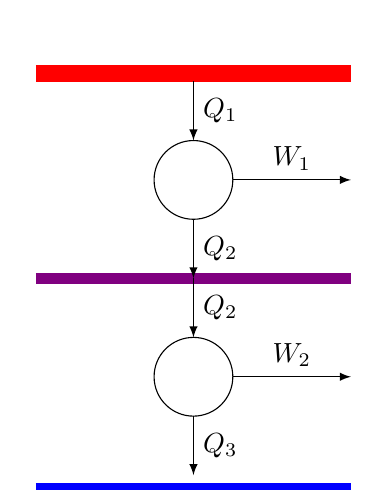
\begin{tikzpicture}
                % Draw the hot, middle, and cold reservoirs with thicker and colored lines
                \draw[line width=6pt, red] (-2,2.1) -- (2,2.1);
                \draw[line width=4pt, violet] (-2,-0.5) -- (2,-0.5);
                \draw[line width=6pt, blue] (-2,-3.2) -- (2,-3.2);
            
                % Draw the circles for the engines
                \draw (0,0.75) circle (0.5);
                \draw (0,-1.75) circle (0.5);
            
                % Draw the arrows and labels for the top engine
                \draw[->] (0,2) -- (0,1.25) node[midway,right] {$Q_1$};
                \draw[->] (0.5,0.75) -- (2,0.75) node[midway,above] {$W_1$};
                \draw[->] (0,0.25) -- (0,-0.5) node[midway,right] {$Q_2$};
            
                % Draw the arrows and labels for the bottom engine
                \draw[->] (0,-0.50) -- (0,-1.25) node[midway,right] {$Q_2$};
                \draw[->] (0.5,-1.75) -- (2,-1.75) node[midway,above] {$W_2$};
                \draw[->] (0,-2.25) -- (0,-3) node[midway,right] {$Q_3$};
            \end{tikzpicture}}              
            \caption{Two Carnot engines connected in series with three reservoirs.}
            \label{fig:twocarnots}
        \end{wrapfigure}
        \begin{equation}
            \frac{Q_1}{Q_3} = \frac{Q_1}{Q_2}\frac{Q_2}{Q_3}
        \end{equation}
        \begin{equation}
            \Rightarrow f(\theta_1,\theta_3) = f(\theta_1,\theta_2)f(\theta_2,\theta_3)
        \end{equation}
        To ensure that $\theta_2$ disappears from the equations, the functions must then take the form $f(\theta_i,\theta_j)=\phi(\theta_i)/\phi(\theta_j)$. Then,
        \begin{equation}
            f(\theta_1,\theta_3) = \frac{\phi(\theta_1)}{\phi(\theta_3)}
        \end{equation}
        so that 
        \begin{equation}
             \frac{Q_1}{Q_3} = \frac{\phi(\theta_1)}{\phi(\theta_3)}
        \end{equation}
\newpage
        This result determines a temperature scale called \textbf{Kelvin Scale}.
        \begin{equation}
            \frac{Q_1}{Q_2} = \frac{T_1}{T_2}
        \end{equation}
        Here, $T_1 \equiv \phi(\theta_1)$ is the definition of the \textbf{Kelvin temperature}. Now, if we set the lower temperature to some well known value we can determine $T_2$ with respect to this value. Let us assume an ideal gas and see how the Kelvin scale relates to the ideal gas temperature. For this, let us go through the full Carnot cycle. In the isothermal processes,
        \begin{equation}
            dU = 0 = \dbar Q - PdV \Rightarrow \dbar Q = PdV.
        \end{equation}
        Then the heat coming in is:
        \begin{equation}
            Q_1 = \int_A^B PdV = nR\theta_1\int_{V_A}^{V_B}\frac{dV}{V} = nR\theta_1\ln\lrp{\frac{V_B}{V_A}}.
        \end{equation}
        Similarly, the heat leaving the system is:
        \begin{equation}
            Q_2 = \int_C^DPdV = nR\theta_2\ln\lrp{\frac{V_D}{V_c}}.
        \end{equation}
        Let us take $Q_2$ to be positive for a while. Since $V_D<V_C$, 
        \begin{equation}
            Q_2 = nR\theta_2\lrp{\frac{V_C}{V_D}}.
        \end{equation}
        Then,
        \begin{equation}
            f(\theta_1,\theta_2) =\frac{T_1}{T_2} = \frac{Q_1}{Q_2} = \frac{nR\theta_1\ln\lrp{V_B/V_A}}{nR\theta_2\ln\lrp{V_C/V_D}} = \frac{\theta_1\ln\lrp{V_B/V_A}}{\theta_2\ln\lrp{V_C/V_D}}.
            \label{eq:kelvinfunc}
        \end{equation}
        Next, we need the relation between volumes. During the adiabatic portions, 
        \begin{equation}
            PV^\gamma = \text{const} \hspace{0.5cm} \text{or} \hspace{0.5cm} \theta V^{\gamma-1}=\text{const}.
        \end{equation}
        Since the $B$ and $C$ are connected through adiabatic processes, 
        \begin{equation}
            \theta_1V_B^{\gamma-1} = \theta_2V_C^{\gamma-1}.
            \label{eq:adiabatic1}
        \end{equation}
        Same also applies to points $D$ and $A$.
        \begin{equation}
            \theta_1V_A^{\gamma-1} = \theta_2V_D^{\gamma-1}
            \label{eq:adiabatic2}
        \end{equation}
        Dividing Equation (\ref{eq:adiabatic1}) by (\ref{eq:adiabatic2}) and taking the logarithm we get,
        \begin{equation}
            (\gamma-1)\ln\lrp{\frac{V_B}{V_A}} = (\gamma-1)\ln\lrp{\frac{V_C}{V_D}}
        \end{equation}
        Substituting this into Equation (\ref{eq:kelvinfunc}),
        \begin{equation}
            \frac{Q_1}{Q_2} = \frac{\theta_1\ln\lrp{V_B/V_A}}{\theta_2\ln\lrp{V_B/V_A}} = \frac{\theta_1}{\theta_2}.
        \end{equation}
        Now with the Kelvin scale, letting $\theta_1 = \theta$ and $\theta_2=\theta_0$
        \begin{equation}
            \frac{T}{T_0} = \frac{\theta_1}{\theta_2} = \frac{\theta}{\theta_0} \Rightarrow T = \theta\lrp{\frac{T_0}{\theta_0}}
        \end{equation}
        This shows that the ideal gas temperature is proportional to the Kelvin temperature. We can choose this constant of proportionality to be 1 and replace $\theta$ with $T$. From now on, we will use the Kelvin scale.
    \section{Definition of Entropy}
    \label{sec:2.2Definitionofentropy}
        We start this section by changing our convention: The heat that exits the system will take a negative sign. We have, therefore,
        \begin{equation}
            \frac{Q_1}{-Q_2} = \frac{T_1}{T_2} \Rightarrow \frac{Q_1}{T_1} + \frac{Q_2}{T_2} = 0
            \label{eq:heatflow}
        \end{equation}
        This is the \textbf{equation of heat flow} in a Carnot cycle. Let us now consider a general reversible closed cycle and analyse it in terms of infinitesimal Carnot cycles. 
        \begin{figure}[H]
            \centering
            \includegraphics[width = 0.4\textwidth]{Entropy_Carnot.png}
            \caption{A general reversible closed cycle in terms of infinitesimal Carnot cycles.}
            \label{fig:generalcycle}
        \end{figure}
        In Figure (\ref{fig:generalcycle}), we have many isothermal and adiabatic stages where the work done in opposite directions cancel each other out. For an infinitesimally small Carnot engine, Equation (\ref{eq:heatflow}) becomes
        \begin{equation}
            \frac{\dbar Q_1}{T_1} + \frac{\dbar Q_2}{T_2} = 0,
        \end{equation}
        which when summed over all Carnot cycles in the continuous limit gives us
        \begin{equation}
            \sum_i\frac{\dbar Q_i}{T_i} = 0 \longmapsto \oint\frac{\dbar Q_\text{rev}}{T} = \Delta S = 0
        \end{equation}
        Therefore, the entropy of a system in a reversible closed cycle is conserved.\\
        Looking at the entropy differential, we see that $TdS = \dbar Q_\text{rev}$. Thus, we can rewrite the internal energy as
        \begin{equation}
            dU = \dbar Q_\text{rev} - dW = TdS - PdV.
        \end{equation}
        By this definition, we can relate the heat capacities to the entropy. Recall that
        \begin{equation}
            C_V = \lrp{\frac{\dbar Q_\text{rev}}{dT}}_V,
        \end{equation}
        then
        \begin{equation}
            C_V = T\lrp{\periv{S}{T}}_V.
        \end{equation}
        Similarly,
        \begin{equation}
            C_P = T\lrp{\periv{S}{T}}_P.
        \end{equation}
        Consider the entropy change in a reversible process at constant pressure.
        \begin{equation}
            \Delta S = \int_i^f\frac{\dbar Q_\text{rev}}{T} = \int_{T_i}^{T_f}C_P(T)\frac{dT}{T}
        \end{equation}
        If the system has a nearly constant $C_P$ over the temperature range of the integral then we get
        \begin{equation}
            \Delta S = C_P\ln\lrp{\frac{T_f}{T_i}}.
        \end{equation}
        A good phenomenon to derive the results that we can use to measure the entropy is the phase transitions. During phase transitions, the system takes in heat but the temperature doesn't change. For a phase transition at constant pressure, we can use the enthalpy function defined in (\ref{sec:1.4thermodynamicfunctions}).
        \begin{equation}
            \Delta H = \Delta(U+PV) = \Delta U + P\Delta V
        \end{equation}
        \begin{equation}
            \Delta U = \Delta Q - P\Delta V \Rightarrow \Delta Q = \Delta U +P\Delta V = \Delta H
        \end{equation}
        \begin{equation}
            \Delta S = \frac{\Delta Q_p}{T_p}=\frac{\Delta H}{T_p}
        \end{equation}
        Therefore, all the heat input goes to increase the enthalpy of the system. We can see a complete phase transition (for example of water) in Figure (\ref{fig:phasetransition})
        \begin{figure}[H]
            \centering
            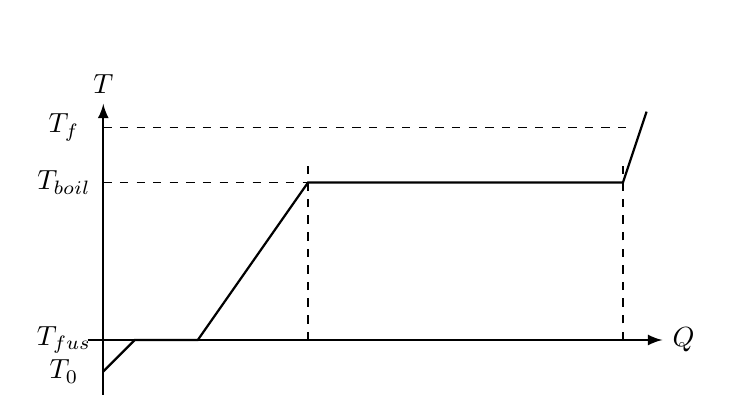
\begin{tikzpicture}
                  \def\ymin{-0.8}
                  \def\ymax{3}
                  \def\xmin{-0.2}
                  \def\xmax{7}
                  \def\t{0.3}    % water/steam transition zone
                  \def\ang{30.4} % angle gradient
                  \coordinate (O) at (0,0);
                  \coordinate (I) at (0.0,-0.4); % ice
                  \coordinate (M) at (0.4,0.0);  % melting
                  \coordinate (W) at (1.2,0.0);  % water
                  \coordinate (E) at (2.6,2,0);  % evaporate
                  \coordinate (S) at (6.6,2.0);  % steam
                  \coordinate (F) at (6.9,2.9);  % final
                  \coordinate (Ex) at ($(E|-O)$); % x evaporation
                  \coordinate (Ey) at ($(E-|O)$); % y evaporation
                  \coordinate (Sx) at ($(S|-O)$); % x steam
                  \coordinate (Fx) at ($(F|-O)$);
                  
                  % AXES
                  \draw[->,thick] (0,\ymin) -- (0,\ymax) node[above=0] {$T$};
                  \draw[->,thick] (\xmin,0) -- (\xmax+0.1,0) node[right=0] {$Q$}; %[\si{J}]
                  \draw[dashed] (Ex) -- (E) --++ (0,0.1*\ymax);
                  \draw[dashed] (Ey) -- (E);
                  \draw[dashed] (Sx) -- (S) --++ (0,0.1*\ymax);
                  \draw[dashed] (E) -- (Ex);
                  \draw[black,thick]
                    (I) -- (M) -- (W)
                      node[midway,above=-1,scale=0.8]{}
                      node[midway,below=-1,scale=0.8]{} --
                    (E)
                      node[pos=0.6,left=1,scale=0.8] {} --
                    (S)
                      node[midway,above=-1,scale=0.8] {}
                      node[midway,below=-1,scale=0.8] {} --
                    (F);
                    \node[black] at (-0.5, -0.4) {$T_0$};
                    \node[black] at (-0.5, 0) {$T_\text{fus}$};
                    \node[black] at (-0.5,2) {$T_\text{boil}$};
                    \draw[dashed] (0,2.7) -- (6.7,2.7);
                    \node[black] at (-0.5, 2.7) {$T_f$};
                \end{tikzpicture}
            \caption{$T-Q$ plot of a complete phase transition.}
            \label{fig:phasetransition}
        \end{figure}
        Therefore the complete change in the entropy of the system is:
        
        \begin{equation}
            S(T_f) = S(T_0) +\int_{T_0}^{T_\text{fus}}C_P\frac{dT}{T} + \frac{\Delta H_\text{fus}}{T_\text{fus}} + \int_{T_\text{fus}}^{T_\text{boil}}C_P\frac{dT}{T} + \frac{\Delta H_\text{boil}}{T_\text{boil}} + \int_{T_\text{boil}}^{T_f}C_P\frac{dT}{T}
        \end{equation}
        
        All the values on the right-hand side of this equation can be measured using calorimetry except $S(T_0)$. Therefore, we can define the value of entropy at $T_0$ by hand. This leads to the Third Law of Thermoydynamics.
        \begin{law*}{The Third Law of Thermodynamics}
            A system's entropy approaches a constant value as its temperature approaches absolute zero. 
        \end{law*}
        Therefore, $S(T_0)$ is defined to be zero for every element in its stable state at the \textbf{absolute zero} $(T_0=0)$. The Third Law has an important corollary that concerns irreversible processes.
    \section{The Law of Increase of Entropy}
        Consider the same system as in Figure (\ref{fig:irrevcarnot})\footnote{Remember that we have changed the sign of the outflowing heat to negative.}. We know by Carnot's Theorem that $\eta_C > \eta_I$. Then,
        
        \begin{equation}
            1-\frac{-Q_2}{Q_1} > 1- \frac{-Q_2'}{Q_1'}
        \end{equation}
        
        From Equation (\ref{eq:heatflow}), 
        
        \begin{equation}
            \frac{-Q_2}{Q_1} = \frac{T_2}{T_1}. 
        \end{equation}
        
        Therefore,
        \begin{equation}
            \frac{-Q_2'}{Q_1'} > \frac{T_2}{T_1}.
        \end{equation}
        
        Now consider infinitesimal heat flow $\dbar Q_1$ and $\dbar Q_2$ as part of this irreversible cycle. With the same procedure as we did in Figure ($\ref{fig:generalcycle}$), for one tiny cycle, we can write the above inequality as
        
        \begin{equation}
            \frac{\dbar Q_1'}{T_1} + \frac{\dbar Q_2'}{T_2} < 0 .
        \end{equation}
        
        If we add together all the infinitesimal cycles, we get
        
        \begin{equation}
            \oint \frac{\dbar Q_\text{irrev}}{T} < 0
        \end{equation}
        
        where $T$ is the temperature of the bath that supplies the heat.
        
        \begin{figure}[H]
            \centering
            \resizebox{0.4\textwidth}{!}{%
            \begin{circuitikz}
                \tikzstyle{every node}=[font=\large]
                \draw [line width = 1.2pt] (12.75,21) .. controls (20.5,26.25) and (16.75,19.75) .. (23.25,21.5);
                \draw [dashed,line width=1.2pt] (12.75,21) .. controls (14.75,16.75) and (19.75,19.25) .. (23.25,21.5);
                \draw [ fill={rgb,255:red,0; green,0; blue,0} , line width=0.2pt ] (23.2,21.5) circle (0.1cm);
                \draw [ fill={rgb,255:red,0; green,0; blue,0} , line width=0.2pt ] (12.75,21) circle (0.1cm);
                \node[black, font = \LARGE] at (12,21) {a}; 
                \node[black, font = \LARGE] at (23.75,21.5) {b};
                \node [font=\LARGE] at (19.5,18.5) {irreversible};
                \node [font=\LARGE] at (17,24) {reversible};
                \draw[->,thick] (10,17) -- (10,25);
                \node [black, font = \LARGE] at (10, 25.7) {$P$};
                \draw[->,thick] (10,17) -- (25,17);
                \node [black, font = \LARGE] at (25.76,17) {$V$};
            \end{circuitikz}}
            \caption{A general cycle broken down into an irreversible and a reversible path.}
            \label{fig:revirrev}
        \end{figure}
        If we suppose that the cycle can be divided into two part: one irreversible and one reversible, as seen in Figure (\ref{fig:revirrev}), we can write the integral as 
        
        \begin{equation}
            \int_a^b\frac{\dbar Q_\text{irrev}}{T} < \int_a^b\frac{\dbar Q_\text{rev}}{T}.
        \end{equation}
        
        We know that we can write the integral along the reversible path in terms of the entropy. 
        
        \begin{equation}
            \int_a^b\frac{\dbar Q}{T} < S(b,a)
        \end{equation}
        
        If $a$ and $b$ are very close such that their temperatures are almost equal, we write $S(b,a) = \delta S$ with $\delta S$ small. Then, we get
        
        \begin{equation}
            \frac{\delta Q_\text{irrev}}{T} < \delta S.
            \label{eq:clausius}
        \end{equation}
        
        The inequality (\ref{eq:clausius}) is called the \textbf{Clausius' inequality}: for an irreversible process the increase in entropy is greater than $\delta Q_\text{irrev}/T$. This is a direct consequence of the Second Law. For a thermally isolated system $\delta Q_\text{irrev} = 0$. Then Clausius' inequality simply becomes $\delta S > 0$. This is known as the \textbf{Law of Increase of Entropy}. Results of this law are:
        \begin{enumerate}
            \item All changes in a thermally isolated system lead to an increase in entropy or keep the entropy same if the system is reversible.
            \item Entropy increases as the system approaches equilibrium where the entropy is at its maximum value. 
            \item At equilibrium there are no more changes as the entropy cannot increase further and it cannot decrease as a function of time. 
            \item Since the entropy is always increasing or staying the same, there exists a direction of time: Positive time is the direction in which the entropy increases in a thermally isolated system.
        \end{enumerate}

        So far we have defined entropy through reversible processes, however since the entropy is defined as $TdS = dU + PdV$ we can also define it for irreversible processes. We thus generalize this definition by stating that it can be applied to any differential change, both reversible and irreversible. There could be processes from a point $a$ to be $b$ where heat and work are not given $TdS$ and $-PdV$. However, even though this is the case, internal energy change is well defined since it is a function of state and independent of the path. We can find a reversible path from $a$ to $b$ and measure the heat added and the temperature along this path. With this, we can determine $dS$ and integrate along the reversible path to find the total change in the entropy. Since entropy is a function of state, this result will be valid for the irreversible path as well. Let us calculate the entropy changes for two irreversible processes. \\
        \\
        Consider an adiabatic system separated by a partition into two equal volumes. The partition is suddenly removed at $t=0$ and an ideal gas is free to expand into whole volume. This is clearly an irreversible process. Since volume doubles, ideal gas law states that the pressure must half. Joule's observations also state that the temperature of a gas freely expanding into vacuum does not change unless there is an external work done on the gas. Therefore, we have
        
        \begin{equation*}
            (P,V,T) \longmapsto (P/2, 2V, T).
        \end{equation*}
        
        We can devise a reversible process equivalent to this process via a piston slowly moving within the same conditions. A gas in a diathermal container is being expanded into a space as piston is slowly moved. The entropy change for this process, as we derived in Equation (\ref{eq:entropydefn}), is then
        
        \begin{equation}
            \Delta S = \frac{3nR}{2}\ln\lrp{\frac{T}{T}} + nR\ln\lrp{\frac{2V}{V}} = nR\ln2
        \end{equation}
        
        Thus, we were able to calculate the entropy change in an irreversible process. 
        
        As an another example consider two identical liquids held at constant volume with a constant heat capacity $C_V$. One at a temperature $T_2$ other at $T_1$. The two liquids are thermally isolated via adiabatic walls and made into contact with one another. As expected, the hotter liquid loses its heat to the colder liquid. Since the total internal energy ($C_VT$) is conserved, temperatures of the two liquids approach $T$ at the equilibrium. We can, therefore, calculate the entropy change in each of the liquids and add them up to find the total change. 
        \begin{equation}
            \Delta S_1 = \int_{T_1}^T\frac{C_VdT}{T} = C_V\ln\lrp{\frac{T}{T_1}}
        \end{equation}
        \begin{equation}
            \Delta S_2 = \int_{T_2}^T\frac{C_VdT}{T} = C_V\ln\lrp{\frac{T}{T_2}}
        \end{equation}
        \begin{equation}
            \therefore \Delta S = \Delta S_1 + \Delta S_2 = C_V\ln\lrp{\frac{T^2}{T_1T_2}}
        \end{equation}
\newpage
    \section{Approach to Equilibrium}
        Assume that a contact is made between two systems ($A$ and $B$) that are not initially at equilibrium with each other. Our question is: how do they approach the equilibrium state ($T$)?
        \begin{equation*}
            A+B\longrightarrow T \hspace{1cm} U_T = U_A + U_B \hspace{1cm} S_T = S_A+S_B
        \end{equation*}
        From the First Law, $dU = TdS - PdV$. However, since the volumes do not change, we have $dU = TdS$ which allows us to write $S=S(U,V)$. 
        Since $U_T$ is a constant, we can write $U_B = U_T-U_A$ to reduce the entropy to depend only on a single variable. 
        \begin{equation}
            S = S(U_A) + S(U_B) \longrightarrow S = S(U_A) + S(U_T-S_A)
        \end{equation}
        Differentiating this equation with respect to time gives us
        \begin{equation}
            \deriv{S}{t} = \periv{S_A}{U_A}\deriv{U_A}{t} + \periv{S_B}{U_B}\deriv{U_B}{t}.
        \end{equation}
        We know that $dU_B/dt = - dU_A/dt$. Then
        \begin{equation}
            \deriv{S}{t} = \deriv{U_A}{t}\lrp{\periv{S_A}{U_A}-\periv{S_B}{U_B}} = \deriv{U_A}{t}\lrp{\frac{1}{T_A}-\frac{1}{T_B}}.
        \end{equation}
        By the Second Law, we get
        \begin{equation}
            \deriv{U_A}{t}\lrp{\frac{1}{T_A}-\frac{1}{T_B}} \geq 0.
        \end{equation}
        We can now investigate three cases:
        \begin{enumerate}
            \item If $T_A=T_B$, the entropy is constant and the system is at thermal equilibrium.
            \item If $T_A>T_B$ then $dU_A/dt$ must be negative. Therefore, energy leaves $A$ and flows into $B$.
            \item If $T_A<T_B$ then $dU_A/dt$ must be positive. Energy leaves $B$ and flows into $A$.
        \end{enumerate}
        In all cases, we see that the energy moves from the hotter body to the colder body. \\
        \\
        Now let us investigate the case in which there is a volume discrepancy rather than a temperature difference. Here we assume $T_A=T_B$ throughout the process. Let us set the problem so that there is a piston between the two systems and as it moves the volume of $A$ increases while the volume of $B$ decreases. The total volume of the two systems however, remains constant. Again, we write
        \begin{equation}
            S = S_A(V_A) + S_B(V_T-V_A).
        \end{equation}
        \begin{equation}
            \Rightarrow \deriv{S}{t} = \deriv{V_A}{t}\lrp{\periv{S_A}{V_A}-\periv{S_B}{V_B}} = \deriv{V_A}{t}\lrp{\frac{P_A}{T_A}-\frac{P_B}{T_B}} \geq
        \end{equation}
\newpage
        From our assumption that the two systems are in a thermal equilibrium, we can again look at three cases.
        \begin{enumerate}
            \item $P_A=P_B$, the entropy is constant and the system is at mechanical equilibrium.
            \item If $P_A>P_B$, $dV_A/dt$ is positive and thus the volume of $A$ increases.
            \item If $P_A<P_B$, $dV_A/dt$ is negative and volume of $A$ decreases.
        \end{enumerate}
        Here, we see that the higher pressure system expands to fill more space. \\
        \\
        Finally, let us look at a permeable wall between the systems and look at the exchange of particles between $A$ and $B$. We again write the total entropy as 
        \begin{equation}
            S = S_A(N_A) + S_B(N_T-N_A)
        \end{equation}
        with the rate of change as
        \begin{equation}
            \deriv{S}{t} = \deriv{N_A}{t}\lrp{\periv{S_A}{N_A}-\periv{S_B}{N_B}}.
        \end{equation}
        We now define a quantity, the \textbf{chemical potential} $\mu$ as
        \begin{equation}
            \mu = -T\lrp{\periv{S}{N}}_{U,V}.
        \end{equation}
        From this definition it follows that
        \begin{equation}
            \deriv{S}{t} = -\deriv{N_A}{t}\lrp{\frac{\mu_A}{T_A}-\frac{\mu_B}{T_B}}\geq 0.
        \end{equation}
        Considering thermal equilibrium with $T_A=T_B$, we again see the three cases. 
        \begin{enumerate}
            \item If $\mu_A = \mu_B$, the entropy is constant and the two systems are at chemical equilibrium. 
            \item If $\mu_A > \mu_B$, $dN_A/dt$ is negative so that the side with the higher chemical potential loses particles and vice versa.
        \end{enumerate}
        In general, the entropy is a function of energy, volume, and the number of particles where we write it as $S=S(U,V,N)$. Then a small change in entropy is given as
        \begin{equation}
            dS = \lrp{\periv{S}{U}}_{V,N} dU + \lrp{\periv{S}{V}}_{U,N}dV + \lrp{\periv{S}{N}}_{U,V}dN 
        \end{equation}
        \begin{equation}
            \therefore dS = \frac{1}{T}dU + \frac{P}{T}dV - \frac{\mu}{T}dN
        \end{equation}
        Here, the term $\mu dN$ can be thought of as \textbf{chemical work}. We will see more of this on later chapters. 
\newpage    
    \section{Exercises}
    \begin{eocproblem*}{2.2 from Bowley \& Sanchez}
        An engine operating between \(300\si{\degree C}\) and \(60\si{\degree C}\) is \(15\%\) efficient. What would be its efficiency be if it were a Carnot engine?
    \end{eocproblem*}
        First of all, we have to convert degree Celsius to Kelvin. \[T_1 = 573\si{K} \hspace{1cm}T_2=333\si{K}.\] For a Carnot engine, we have \(Q_1/Q_2 = T_1/T_2\) and \(\eta = 1-T_2/T_1\). Then,
        \begin{equation}
            \eta = 1-\frac{T_2}{T_1} = 1 -\frac{333}{573} = 0.418.
        \end{equation}
        Then this engine would have an efficiency of \(42\%\) had it been a Carnot engine.
        
    \begin{eocproblem*}{2.6 from Bowley \& Sanchez}
        An ideal gas with \(\gamma=1.5\) is used as the working substance in the cylinder of an engine undergoing a Carnot cycle. The temperature of the hot reservoir is \(240\si{\degree C}\), and that of the cold is \(50\si{\degree C}\). The gas is expanded isothermally at $240\si{\degree C}$ from a pressure of $10\si{atm}$ and a volume of $1\si{L}$ to a pressure of $4\si{atm}$ and a volume of $2.5\si{L}$. Between what limits of pressure and volume does the gas operate when it is in thermal equilibrium with the cold reservoir?    
    \end{eocproblem*}
    
        Again converting the temperatures into Kelvin, we have $T_1 = 513\si{K}$ and $T_2 = 323\si{K}$. For the isothermal process we know that $PV=nRT=$ constant and that during the isothermal expansion $T=T_1$ while during the isothermal compression, $T=T_2$. Now imagine the Carnot cycle with isothermal expansion from $A$ to $B$ along the path $(1)$, adiabatic expansion from $B$ to $C$ along path the $(2)$, isothermal compression from $C$ to $D$ along path the $(3)$, and adiabatic compression from $D$ to $A$ along the path $(4)$. Since the thermal equilibrium with the cold reservoir occurs along the isothermal compression, the limits of pressure and volume asked in question are the values of pressure and volume at points $C$ and $D$. 
        
        Now, let us look at the adiabatic processes which correspond to paths $(2)$ and $(4)$. Along these paths, $PV^\gamma =$ constant and thus, $P \propto V^{-\gamma}$. Moreover since we have an ideal gas, $PV = nRT$. 
        
        \begin{equation}
            PV \propto T \Rightarrow V^{1-\gamma} \propto T \Rightarrow TV^{\gamma-1} = \text{const}.
        \end{equation}
        
        Then at points $B$ and $C$, we have
        
        \begin{equation}
            T_BV_B^{\gamma-1} = T_CV_C^{\gamma-1} \Rightarrow T_BV_B^{0.5} = T_CV_C^{0.5}.
        \end{equation}
        
        Since at $B$ we have the temperature of the hot reservoir and at $C$ we have the temperature of the cold reservoir and we know that $V_B = 2.5\si{L}$, we can write
        
        \begin{equation}
            513\si{K}\sqrt{2.5\si{L}} = 323\si{K}\sqrt{V_C}.
        \end{equation}
        \begin{equation}
            \Rightarrow \sqrt{V_C} = \frac{513}{323}\sqrt{2.5\si{L}} \Rightarrow V_C \approx 6.3\si{L}
        \end{equation}
        
        During the adiabatic expansion, $P_BV_B^\gamma = P_CV_C^\gamma$. 
        
        \begin{equation}
            4\si{atm}(2.5\si{L})^{1.5} = P_C(6.3\si{L})^{1.5}\Rightarrow P_C = \lrp{\frac{2.5}{6.3}}^{1.5}4\si{atm} \approx 1\si{atm}
        \end{equation}
        
        During the adiabatic compression we again have $TV^{\gamma-1}=$ const. Therefore,
        
        \begin{equation}
            T_A(V_A)^{0.5} = T_D(V_D)^{0.5} \Rightarrow 513\si{K}(1\si{L})^{0.5} = 323\si{K}(V_D)^{0.5}.
        \end{equation}
        \begin{equation}
             \Rightarrow V_D = \lrp{\frac{513}{323}}^2\times 1\si{L} \approx 2.5\si{L}
        \end{equation}
        
        Finally, we look at $PV^\gamma=$ const condition along the adiabatic compression.
        
        \begin{equation}
            10\si{atm}(1\si{L})^{1.5} = P_D(2.5\si{L})^{1.5} \Rightarrow P_D = \lrp{\frac{1}{2.5}}^{1.5}10\si{atm} \approx 2.53\si{atm}
        \end{equation}
        Then, the limits are
        \begin{equation}
            P_C = 1\si{atm} \hspace{0.5cm} V_C = 6.3\si{L} \hspace{1cm}\&\hspace{1cm} P_D = 2.53\si{atm} \hspace{0.5cm} V_D = 2.5\si{L}
        \end{equation}

    \begin{eocproblem*}{2.8 from Bowley \& Sanchez}
        A certain amount of water of heat capacity $C$ is at a temperature of $0\si{\degree C}$. It is placed in contact with a heat bath at $100\si{\degree C}$, and the two come into thermal equilibrium.
        \begin{enumerate}[label = (\alph*)]
            \item What is the entropy change of the universe?
            \item The process is now divided into two stages: first, the water is placed in contact with a heat bath at $50\si{\degree C}$ and comes into thermal equilibrium; then it is placed in contact with the heat bath at $100\si{\degree C}$. What is the entropy change of the universe?
            \item The process is divided into four stages with heat baths at $25,50,75,$ and $100\si{\degree C}$. What is the entropy change of the universe in this case?
            \item If we were to continue this subdivision into an infinite number of heat baths, what would be the entropy change of the universe?
        \end{enumerate}
    \end{eocproblem*}
    
        Before doing each of the calculations, we have to convert the degrees into Kelvin.
        \begin{enumerate}[label = (\alph*)]
            \item Using the definition of entropy,
            
            \begin{equation}
                \Delta S_\text{water} = \int_{T_1}^{T_2}\frac{dQ}{T} = \int_\text{273K}^\text{373K} \frac{CdT}{T} = C\ln\lrp{\frac{373}{273}}=0.31C
            \end{equation}
            
            and     
            \begin{equation}
                \Delta S_\text{bath} = -\frac{\Delta Q}{T} = -\frac{C\Delta T}{T_2} = -C\frac{100}{373} = -0.26C.
            \end{equation}
            
            Then the entropy change of the universe is 
            
            \begin{equation}
                \Delta S_\text{universe}=\Delta S_\text{water}+\Delta S_\text{bath} = 0.31C-0.26C = 0.05C.
            \end{equation}
        \end{enumerate}
        
    \begin{eocproblem*}{2.11 from Bowley \& Sanchez}
        Two identical bodies with heat capacities at constant volume which vary linearly with temperature, $C=bT$, are thermally isolated. One is at a temperature of $100 \si{K}$, the other is at $200\si{K}$. They are placed in thermal contact and come to thermal equilibrium. What is the final temperature of the two bodies, and what is the entropy change of the system?
    \end{eocproblem*}
        Since the bodies have constant volume, we use $C_V$. Therefore, for each body, the internal energy is
        
        \begin{equation}
            C_V = bT = \periv{U}{T} \Rightarrow dU = b\int T dT \Rightarrow U = \frac{bT^2}{2} + U_0(V).
        \end{equation}
        
        Then the initial total internal energy for the composite system is
        
        \begin{equation}
            U_i = \frac{b}{2}(T_1^2+T_2^2) + 2U_0.
        \end{equation}
        
        Since there is no work being done or heat entering the system, $\Delta U = 0$. 
        
        \begin{equation}
            U_f = \frac{b}{2}(T_f^2 + T_f^2) + 2U_0 = U_i
        \end{equation}
        \begin{equation}
            \frac{b}{2}(T_1^2+T_2^2) + 2U_0 = bT_f^2 + 2U_0
        \end{equation}
        \begin{equation}
            \Rightarrow \frac{T_1^2+T_2^2}{2} = T_f^2
        \end{equation}
        
        Substituting the values, the final temperature is
        
        \begin{equation}
            T_f = \sqrt{\frac{100^2+200^2}{2}} = \sqrt{5000+20000} = \boxed{158.1\si{K} }
        \end{equation}
        
        Now we calculate the entropies via the relation between the entropy and the heat capacity.
        
        \begin{equation}
            C_V = T\lrp{\periv{S}{T}}_V = bT \Rightarrow \periv{S}{T} = b \hspace{0.5cm} \therefore S = bT + S_0 
        \end{equation}
        
        Total initial and final entropies are then calculated as
        
        \begin{equation}
            S_i = S_1+S_2 = b(T_1+T_2) + 2S_0 \hspace{1cm} S_f = 2bT_f + 2S_0
        \end{equation}
        \begin{equation}
            \Rightarrow \Delta S = S_f-S_i = 2bT_f - b(T_1+T_2) = b(2\times158.1-100-200) = \boxed{16.27b \si{J/K}}
        \end{equation}

    \begin{eocproblem*}{2.19 from Bowley \& Sanchez}
        Two identical finite bodies of constant volume and constant heat capacity at constant volume, $C_V$, are used to drive a heat engine. Their initial temperatures are $T_1$ and $T_2$. Find the maximum amount of work which can be obtained from the system. [Hint: The maximum amount of work can be drawn when there is no entropy change.]
    \end{eocproblem*}
        Using the definition of $C_V$ via entropy, we get
        \begin{equation}
            C_V = T\periv{S}{T} \Rightarrow dS = C_V\frac{dT}{T}.
        \end{equation}
        Then the change in the entropy is
        \begin{equation}
            \Delta S = \Delta S_1 + \Delta S_2 = \int dS_1 + \int dS_2 = C_V\lrp{\int_{T_1}^{T_f}\frac{dT}{T}+\int_{T_2}^{T_f}\frac{dT}{T}} \notag
        \end{equation}
        \begin{equation}
            = C_V\lrp{\ln\lrp{\frac{T_f}{T_1}}+\ln\lrp{\frac{T_f}{T_2}}} = C_V\ln\lrp{\frac{T_f^2}{T_1T_2}} = 0.
        \end{equation}
        \begin{equation}
            \Rightarrow \frac{T_f^2}{T_1T_2} = 1 \Rightarrow T_f = \sqrt{T_1T_2}
        \end{equation}
        Now we use the First Law to calculate the work: $W = -\Delta U$. We obtain the internal energy via the heat capacity.
        \begin{equation}
            C_V=\periv{U}{T} \Rightarrow U = C_VT + U_0 
        \end{equation}
        Then the total initial and final internal energies are
        \begin{equation}
            U_i = C_V(T_1+T_2) + 2U_0 \hspace{0.5cm} \& \hspace{0.5cm} U_f = 2C_VT_f + 2U_0
        \end{equation}
        Finally by combining these, we get the work done.
        \begin{equation}
           \boxed{ W = -\Delta U = U_i-U_f = C_V(T_1+T_2-2\sqrt{T_1T_2})}
        \end{equation}
\newpage
    \begin{eocproblem*}{2.20 from Bowley \& Sanchez}
        The differential of the internal energy of a surface of a liquid with surface tension $\gamma$ and area $A$ may be written as \[dU = TdS + \gamma dA.\] Write down the corresponding form of the Helmholtz free energy, \(F=U-TS\). Using the fact that these equations involve inexact differentials, derive the Maxwell relation \[\lrp{\periv{S}{A}}_T = -\lrp{\periv{\gamma}{T}}_A.\] The internal energy and the entropy are proportional to the area \(A\). show that the internal energy per unit area is \[u(T) = \frac{U}{A} = \gamma - T\lrp{\periv{\gamma}{T}}_A.\]
    \end{eocproblem*}
        We begin by writing \(dF\) and substituting the given \(dU\).
        \begin{equation}
            dF = dU - TdS - SdT = TdS + \gamma dA - TdS - SdT = \gamma dA - SdT
        \end{equation}
        Then for constant area and constant temperature, we can write
        \begin{equation}
            S=-\lrp{\periv{F}{T}}_A \hspace{1cm }\gamma = \lrp{\periv{F}{A}}_T.
        \end{equation}
        Differentiating the entropy with respect to area and the tension  with respect to the temperature, we obtain the Maxwell relation.
        \begin{equation}
            -\periv{S}{A} = \periv{^2F}{A\del T} \hspace{1cm} \periv{\gamma}{T} = \periv{^2F}{T\del A} \hspace{1cm }            \boxed{\therefore \periv{S}{A}=-\periv{\gamma}{T}}
        \end{equation}
        To find the internal energy per unit area, we start with \(dU=TdS+\gamma dA\) and writing \(dS\) as \(dS=\del_TSdT+\del_ASdA\). Then, integrating both sides,
        \begin{equation}
            \int dU = \int T\periv{S}{T}dT + \int T\periv{S}{A}dA + \int\gamma dA.
        \end{equation}.
        Since \(u\propto A\), \(S\propto A\). Then, \(\del_TS=0\). We now obtain
        \begin{equation}
            U = \int\lrp{T\periv{S}{A}+\gamma}dA.
        \end{equation}
        Since the internal energy is given as an integral over area, the internal energy per unit area is just the integrand of this integral. Using the Maxwell relation we obtained previously, we get
        \begin{equation}
            \boxed{\therefore u(T) = \gamma -T\periv{\gamma}{T}}
        \end{equation}
\chapter{Probability and Statistics}

    Before we delve into statistical mechanics, we first have to go through the mathematics on which the subject is built. Before starting this chapter, let us make a few definitions.
    \paragraph{Trial:}A process at the end of which one obtains certain outcomes.
    \paragraph{Event:}Each outcome of a trial.
    \paragraph{Probability:}Measure of likelihood of occurrence of an event.
    There are two ways of asigning a probability to an event. First of these is the statistical probability.
    \paragraph{Statistical Probability:}Probability assigned to events based on relative frequency. Given that an experiment with $N$ trials yields $n_A$ occurrences of event $A$, the \textbf{probability} $P(A)$ of event $A$ occurring is
    \begin{equation}
        P(A) = \lim_{N\to\infty}\frac{n_A}{A}.
    \end{equation}
    In real experiments, it is obvious that one cannot conduct infinitely many trials. However, upon conducting a large amount of experiments one may utilise other methods to produce probabilities.
    
    The second way to assign a probability is the classical probability.
    \paragraph{Classical (A Priori) Probability:}Probability assigned to an event before it takes place, assigning equal likelihood to all outcomes.
\newpage
    \section{Axioms of Probability Theory}
        To define an axiomatic system of a theory of probability, we have to borrow some ideas from set theory. Let us take the die as an example and consider three events $A,B$, and $C$. 
        \begin{itemize}
            \item \textbf{Event A:} An odd number smaller than 4
            \item \textbf{Event B:} An odd number smaller than 2
            \item \textbf{Event S:} Certain event. Any number between 1 and 6.
        \end{itemize}
        \begin{figure}[H]
            \centering
                \tikzset{every picture/.style={line width=0.75pt}} %set default line width to 0.75pt        
                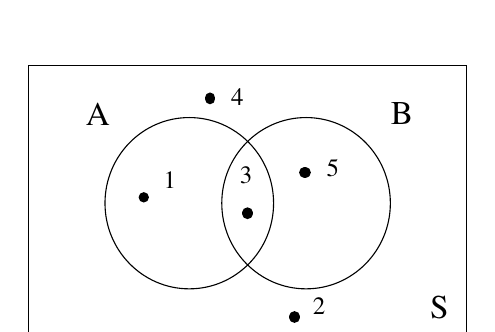
\begin{tikzpicture}[x=0.75pt,y=0.75pt,yscale=-1,xscale=1]
                    %uncomment if require: \path (0,300); %set diagram left start at 0, and has height of 300
                    
                    %Shape: Rectangle [id:dp5602169304393213] 
                    \draw   (100,41.67) -- (311,41.67) -- (311,174) -- (100,174) -- cycle ;
                    %Shape: Ellipse [id:dp4357935586445133] 
                    \draw   (136.98,107.83) .. controls (136.98,85.04) and (155.16,66.57) .. (177.59,66.57) .. controls (200.02,66.57) and (218.21,85.04) .. (218.21,107.83) .. controls (218.21,130.62) and (200.02,149.1) .. (177.59,149.1) .. controls (155.16,149.1) and (136.98,130.62) .. (136.98,107.83) -- cycle ;
                    %Shape: Ellipse [id:dp5865551607027422] 
                    \draw   (193.25,107.83) .. controls (193.25,85.04) and (211.43,66.57) .. (233.86,66.57) .. controls (256.29,66.57) and (274.47,85.04) .. (274.47,107.83) .. controls (274.47,130.62) and (256.29,149.1) .. (233.86,149.1) .. controls (211.43,149.1) and (193.25,130.62) .. (193.25,107.83) -- cycle ;
                    %Shape: Free Drawing [id:dp6682110093205644] 
                    \draw  [line width=3.75] [line join = round][line cap = round] (155.67,105) .. controls (155.67,105) and (155.67,105) .. (155.67,105) ;
                    %Shape: Free Drawing [id:dp2277868619577088] 
                    \draw  [line width=3.75] [line join = round][line cap = round] (205.67,112.33) .. controls (205.67,112.56) and (205.67,112.78) .. (205.67,113) ;
                    %Shape: Free Drawing [id:dp833320635160391] 
                    \draw  [line width=3.75] [line join = round][line cap = round] (233.67,93) .. controls (233.44,93) and (233.22,93) .. (233,93) ;
                    %Shape: Free Drawing [id:dp7574780843900116] 
                    \draw  [line width=3.75] [line join = round][line cap = round] (228.33,162.33) .. controls (228.33,162.56) and (228.33,162.78) .. (228.33,163) ;
                    %Shape: Free Drawing [id:dp7194338325314746] 
                    \draw  [line width=3.75] [line join = round][line cap = round] (187.67,57) .. controls (187.67,57.22) and (187.67,57.44) .. (187.67,57.67) ;
                    
                    % Text Node
                    \draw (126.49,58.57) node [anchor=north west][inner sep=0.75pt]   [align=left] {{\fontfamily{ptm}\selectfont {\large A}}};
                    % Text Node
                    \draw (273.51,57.84) node [anchor=north west][inner sep=0.75pt]   [align=left] {{\fontfamily{ptm}\selectfont {\large B}}};
                    % Text Node
                    \draw (292.39,150.98) node [anchor=north west][inner sep=0.75pt]   [align=left] {{\fontfamily{ptm}\selectfont {\large S}}};
                    % Text Node
                    \draw (164,91.33) node [anchor=north west][inner sep=0.75pt]   [align=left] {{\small {\fontfamily{ptm}\selectfont 1}}};
                    % Text Node
                    \draw (200.67,88.67) node [anchor=north west][inner sep=0.75pt]   [align=left] {{\small {\fontfamily{ptm}\selectfont 3}}};
                    % Text Node
                    \draw (235.86,152.1) node [anchor=north west][inner sep=0.75pt]   [align=left] {{\small {\fontfamily{ptm}\selectfont 2}}};
                    % Text Node
                    \draw (242.53,85.43) node [anchor=north west][inner sep=0.75pt]   [align=left] {{\small {\fontfamily{ptm}\selectfont 5}}};
                    % Text Node
                    \draw (196.53,51.43) node [anchor=north west][inner sep=0.75pt]   [align=left] {{\small {\fontfamily{ptm}\selectfont 4}}};
                \end{tikzpicture}
            \caption{A Venn diagram of events $A$, $B$, and $S$.}
            \label{fig:venndiagram}
        \end{figure}
        Here, we can see that Event $S$ is the whole set of events. If we want to get the Event $A$ OR Event $B$, we have $A\cup B = \{1,3,5\}$ and if we want to get both the Event $A$ AND Event $B$, we have $A\cap B = \{3\}$. \\
        \\
        Now, let us state the axioms of the probability theory.
        \begin{enumerate}
            \item The probability $P(A)$ of an event $A$ is a non-negative number assigned to that event.
            \begin{equation}
                P(A)\geq 0
            \end{equation}
            \item The probability of a certain event is 1.
            \begin{equation}
                P(S) = 1
            \end{equation}
            \item If $A\cap B = \emptyset$, where $\emptyset$ denotes the empty set, then
            \begin{equation}
                P(A+B) = P(A) + P(B)
            \end{equation}
        \end{enumerate}
        Axiom (3) describes the \textbf{mutually exclusive} events: Events that cannot happen at the same time.
        \begin{problem}{Consider a box with 3 green, 5 blue, and 4 red balls. A ball is drawn at random. What is the probability that the ball drawn is either green or blue?}
        bSince there are 12 balls in total we have \[P(G) = \frac{3}{12} \hspace{1cm} P(B) = \frac{5}{12.}\] And since both events cannot happen simultaneously, they are mutually exclusive events and thus \[ P(B+G) = \frac{8}{12} = \frac{2}{3}.\]
        \end{problem}
        \begin{problem}{Two dice are rolled. What is the probability that sum of two numbers is 7?}
           bLet us list all possibilities: $\{2,3,4,5,6,7,8,9,10,11,12\}$. Then, we get $P = 1/N = 1/11$. However, this is a wrong answer simply because the event that the sum of the numbers is 7 depends on the pair of trials. The correct way to count the desired outcomes is:$ \{(1,6),(2,5),(3,4),(4,3),(5,2),(6,1)\}$. Since the total number of pairs is $6^2=36$, we get \[P =6/36 = 1/6.\]
        \end{problem}
        One can note the in Problem 3, not all outcomes are equally likely. So a question is: How does one assign a priori probability to events?
        \paragraph{Principle of Insufficient Reason / Principle of Indifference: }In the absence of any a priori knowledge, we must assume that each relevant outcome $A_i$ must be equally likely.
        \paragraph{Independent Outcomes:} If the probability of both events occurring is the product of single event probabilities then the two events are \textbf{independent} or \textbf{uncorrelated}. 
        \begin{equation}
            P = \prod_i P_i
        \end{equation}
    \section{Counting the Number of Events}
        The simple act of counting the number of ways in which the events can occur leads to the definition of important concepts like arrangements, permutations, and combinations. Let us begin with arrangements. Here, a number of objects is arranged along a line. The number of possible arrangements change depending on the objects that are arranged are similar or not.\\
        \begin{enumerate}
            \item The number of ways of arranging $n$ dissimilar objects in a line is $n!$.
            \item The number of ways of arranging $n$ objects, $p$ of which are identical along a line is $n!/p!$.
        \end{enumerate}
        If we'd like to generalize the second arrangement, if there are $n$ objects $p_1$ of which are one kind, $p_2$ of which are another kind and so on, then the number of ways in which the objects can be arranged along a line is
        
        \begin{equation}
            \frac{n!}{\prod_ip_i!}
        \end{equation}
        
        Now let us consider the permutations. These are the cases where a number of objects are chosen out of a larger set of objects and where one choice is independent of the other. Choosing $r$ objects out of $n$ objects is called the \textbf{permutation} of $r$ out of $n$. We write the number of permutations as
        
        \begin{equation}
            ^nP_r = \frac{n!}{(n-r)!}.
        \end{equation}
        
        Finally, we have the combinations where again $r$ objects are chosen out of $n$ objects but the order of the choice does not matter. Consider 10 pieces of chalk where three are chosen. Then by Equation 3.2.2,
        
        \begin{equation}
            ^{10}P_3 = \frac{10!}{(10-3)!} = \frac{10!}{7!} = 10\times9\times8.
        \end{equation}
        
        Now let us name the chosen chalks as $A,B$, and $C$. Then there are $3!$ orders in which we can select these three chalks. Here, we define the \textbf{combination} as
        
        \begin{equation}
            3!^{10}C_3 = ^{10}P_3.
        \end{equation}
        
        In general, the number of combinations of $r$ objects out of $n$ is
        
        \begin{equation}
            ^nC_r=\frac{n!}{r!(n-r)!}.
        \end{equation}
        
        Now let us define the concept of a box. Upon choosing any amount $r$ objects out of $n$ objects, we put the chosen objects into a box so that they cannot be chosen anymore. Then, another $q$ amount of objects are chosen from what is now $n-r$ objects and again put into a box. This goes on until all the objects are separated into boxes. In general, the number of arrangements for $N$ pieces of objects with $n_i$ in box $i$ is 
        
        \begin{equation}
            W = \frac{N!}{\prod_in_i!}.
            \label{eq:box}
        \end{equation}
        
        Equation (\ref{eq:box}) can be used to work out the total number of ways energy can be arranged between different quantum mechanical states levels in $N$ identical systems where $n_i$ represent the number of times this quantum state is occupied.
    \section{Distributions}
        The outcomes of events are not, in general, uniform. When looking at the statistical data of an experiment, over which one may assign a statistical probability, in a plot of outcomes versus occurrences different shaped plots appear for different cases. These plots are called \textbf{probability distribution functions (PDFs)} or just distributions in short. Let $X$ be a variable that takes on numerical values determined by the outcome of a random experiment. Such variables are called \textbf{random variables}. Random variables can either take discrete values (which are then called \textbf{discrete random variables}) or can lie on a continuous spectra. A probability distribution function $P(X=x)$ express the probability that a random variable $X$ takes on a value $x$. There are two main properties of PDFs.
        \begin{enumerate}
            \item Since the probability is a non-negative value, so must the value of a PDF at a value $x$. \(P(X=x) \geq 0\) \( \forall X\)
            \item The probability that the experiment yields a result is always unity. Thus, the sum of all possible values taken by a PDF must be unity. \(\sum_xP(x)=1\)
        \end{enumerate}

        Rather than looking at the probability of a single outcome, one can also define a function that gives the probability that the outcome is greater than a set amount, i.e. the probability that $X$ is less than or equal to $x_0$. Such functions are called \textbf{cumulative probability functions}.\\
        \\
        In their essence, PDFs are just histograms with continuous PDFs having the limit as the bin size goes to zero or the bin count goes to infinity. Therefore, we can calculate the same important quantities for PDFs just as we can do for histograms.\\
        \\
        Let us consider an experiment where the possible outcomes are binned in a histogram. Here we can describe the results of the experiment using 
        \begin{itemize}
            \item \textbf{Mean:} The arithmetic average of the outcomes. 
            \begin{equation}
                \bar{x} = \frac{1}{N}\sum_i^N x_i
            \end{equation}
            \item \textbf{Median:} The value at the middle in an ordered list of outcomes.
            \item \textbf{Mode:} The outcome that occurs the most often.
        \end{itemize}
        These three measures are called \textbf{central tendency measures}. If the distribution is binned, then the mean is given by
        \begin{equation}
            \bar{x} = \frac{1}{N}\sum_i^Nn_ix_i
            \label{eq:defmean}
        \end{equation}
        where $N$ is the amount of trials and $n_i$ is the number in bin $i$. By defining the statistical probability $p_i = n_i/N$ and taking the limit as $N$ goes to infinity, we can write Equation (\ref{eq:defmean}) as
        \begin{equation}
            \bar{x} = \sum_i^Np_ix_i.
        \end{equation}
        Although the mean value in a PDF provides valuable information, it cannot be used alone to define or make predictions about an experiment. To quantify how much the values deviate from the average we define two quantities. 
        \begin{itemize}
            \item \textbf{Variance:} Average of squared deviations of values from the mean.
            \begin{equation}
                (\Delta x)^2 = \frac{1}{N}\sum_i^N(x_i-\bar{x})^2
            \end{equation}
            \item \textbf{Standard Deviation:} Square root of the variance.
            \begin{equation}
                \Delta x = \sqrt{\frac{1}{N}\sum_i^N(x_i-\bar{x})^2}
            \end{equation}
        \end{itemize}
        Similarly, we can use the sstatistical probability to write the variation as 
        \begin{equation}
            (\Delta x)^2 = \sum_ip_i(x_i-\bar{x})^2.
            \label{eq:stddevdefn}
        \end{equation}
        Although there are several important PDFs that are generally used throughout physics, the most common one is the \textbf{Gaussian / Normal Distribution}. This is due to the \textbf{Central Limit Theorem (CLT)}.
        \begin{theorem}{Central Limit Theorem}
            bUnder appropriate conditions, the distribution of a normalized version of the sample mean converges to a standard normal distribution.
        \end{theorem}
        In general, the appropriate conditions are taken as the cases where the number of samples is larger than 30. If the Gaussian distribution is continuous, it is given by the function
        \begin{equation}
            p(x) = \frac{e^{-(x-\mu)^2/2\sigma^2}}{\sqrt{2\pi}\sigma}.
            \label{eq:gaussian}
        \end{equation}
        This distribution, as suggested by its name, is a Gaussian function and thus is bell-shaped. This is seen in Figure (\ref{fig:gaussian}).
        \begin{figure}[H]
            \centering
            \resizebox{0.75\textwidth}{!}{%
            \begin{tikzpicture}
                  \begin{axis}[
                    width = 17.5cm,
                    height = 7.25cm,
                    xmin = -4.5, xmax = 4.5,
                    ymin = 0,
                    axis x line = bottom, % the * suppresses the arrow tips
                    hide y axis,
                    xtick = {-1,...,1},
                    % xtick = {0},
                    % tick label style = {color=white}, % uncomment this line and change all other
                    % xtick tags to remove x-axis markings
                    xtick align = outside,
                    xticklabels = {
                      $(\bar{x}-\Delta x)$, $\vphantom{(}\bar{x}$, $(\bar{x}+\Delta x)$}, % comment this if uncomment above;
                        %commenting this without uncommenting above makes markings integers
                  ]
                  % This draws the vertical lines
                  \pgfplotsinvokeforeach {-1,0,1} {
                    \draw[black, thick] (axis cs: #1,-1)
                      -- (axis cs: #1,{(1/sqrt(2*pi))*exp((-1/2)*(#1)^2)});
                  }
                        
                  % This draws the main curve
                  \addplot [
                    domain = -4.5:4.5, 
                    samples = 251, 
                    color = red,
                    very thick,
                    name path = dist
                  ]
                  {(1/sqrt(2*pi))*exp((-1/2)*x^2)};

                  \addplot [
                    domain = -1.22:1.22,
                    samples = 3,
                    color = blue,
                    very thick
                  ]
                  {1/(2*sqrt(2*pi))};
                \end{axis}
                \end{tikzpicture}
                }
            \caption{Shape of the Gaussian distribution. The blue line indicates the FWHM.}
            \label{fig:gaussian}
        \end{figure}
\newpage
        Now, note that the maximum value of this function is at $x=\mu$. Since this value has to be the mean of the distribution, we get $\mu = \bar{x}$. An important interval of outcomes is the \textbf{Full Width at Half Maximum (FWHM)}. This interval is the width of the "bell" where the height is at the half of the maximum height. To calculate this let $x=\bar{x}$ since we know that $P(\bar{x})$ is the maximum value of the distribution.
        \begin{equation}
            p(\bar{x}) = \frac{e^{-(\bar{x}-\bar{x})^2/2\sigma^2}}{\sigma\sqrt{2\pi}} = \frac{1}{\sigma\sqrt{2\pi}} \Rightarrow \text{HM} = \frac{1}{2\sqrt{2\pi}\sigma}
        \end{equation}
        Since the distribution is symmetric around $\bar{x}$, there will be two values of $p(x)$ corresponding to $x=x_\text{HM}$. 
        \begin{equation}
            p(x_\text{HM}) = HM \Rightarrow \frac{e^{-(x_1-\bar{x})^2/2\sigma^2}}{\sqrt{2\pi}\sigma} = \frac{1}{2\sqrt{2\pi}\sigma} \Rightarrow \frac{(x_1-\bar{x})^2}{2\sigma^2} = \ln2 
        \end{equation}
        \begin{equation}
            (x_\text{HM}-\bar{x})^2 = 2\sigma^2\ln2
        \end{equation}
        \begin{equation}
            \therefore x_\text{HM} = \mp\sqrt{2\ln2}\sigma+\bar{x}
        \end{equation}
        This is the full width at half maximum.
        Recall the second property of the PDFs that $\sigma_xP(x)=1$. However, this may not be the case in general. This property is called the \textbf{normalization} and if a PDF is not normalized at the beginning. It has to be normalized before solving any questions. At the continuous limit, the discrete summation becomes an integral.
        
        \begin{equation}
            \int_\mathcal{\tau}P(x)d\tau = \frac{1}{\sqrt{2\pi}\sigma}\int_{-\infty}^{\infty}dxe^{-(x-\bar{x})^2/2\Delta x^2} \notag 
        \end{equation}
        \begin{equation}
            = \frac{1}{\sqrt{2\pi}\sigma}\sqrt{2\sigma^2\pi} = 1
        \end{equation}
        Therefore, the definition of the normal distribution given in Equation (\ref{eq:gaussian}) is already normalized. Finally, let us now calculate the standard deviation in the normal distribution. For a continuous distribution, Equation (\ref{eq:stddevdefn}) becomes
        \begin{equation}
            (\Delta x)^2=\int_{-\infty}^\infty p(x)(x-\bar{x})^2 dx.
        \end{equation}
        Then,
        \begin{equation}
            (\Delta x)^2 = \frac{1}{\sigma\sqrt{2\pi}}\int_{-\infty}^{\infty}\exp\lrp{-\frac{(x-\bar{x})^2}{2\sigma^2}}(x-\bar{x})^2dx
        \end{equation}

        Let us define a variable $\alpha$ and do a u-substitution.
        \begin{equation}
            \alpha = \frac{1}{2\sigma^2} \hspace{1cm} u=x-\bar{x}\Rightarrow du=dx
        \end{equation}
        This gives us
        \begin{equation}
            (\Delta x)^2 = \frac{1}{\sigma\sqrt{2\pi}}\int_{-\infty}^\infty e^{-\alpha u^2}u^2du. = -\frac{1}{\sigma\sqrt{2\pi}}\periv{}{\alpha}\int_{-\infty}^\infty e^{-\alpha u^2}du
        \end{equation}
        This is the Gaussian integral that we know how to solve. 
        \begin{equation}
            (\Delta x)^2 = -\frac{1}{\sigma\sqrt{2\pi}}\periv{}{\alpha}\lrp{\sqfrac{\pi}{\alpha}} = -\frac{1}{\sigma\sqrt{2}}\periv{\alpha^{-1/2}}{\alpha} = \frac{1}{2\sqrt{2}\sigma}\alpha^{-3/2}
        \end{equation}
        Substituting the $\alpha$ back,
        \begin{equation}
            (\Delta x)^2 = \frac{1}{2\sqrt{2}\sigma}\lrp{\frac{1}{2\sigma^2}}^{-3/2} = \frac{\sqrt{8\sigma^6}}{\sqrt{8}\sigma} = \sigma^2.
        \end{equation}
        Thus, we see that $\Delta x = \sigma$. Then, we can write the Gaussian distribution as
        \begin{equation}
            p(x) = \frac{\exp\lrp{-\frac{(x-\bar{x})^2}{2(\Delta x)^2}}}{\sqrt{2\pi}\Delta x}.
        \end{equation}
        
\chapter{Ideas of Statistical Mechanics}

Statistical mechanics deals with the cause and effect relationship between micro and macro states.
\paragraph{Ensemble:} A (imaginary) collection of $\Gamma$ number of systems with the same macro states but different time dependent micro states.

%insert tikz images


\paragraph{Example:}

$\underbrace{\stkout{\updownarrows\downuparrows \updownarrows \upuparrows \updownarrows\downdownarrows \cdots}}_{N\textrm{ spins (micro state)}} \quad \longleftrightarrow \quad \underbrace{m=n_\uparrow + n_\downarrow}_\textrm{magnetization (macro state)}$

\begin{problem}{How many micro states are there for a macro state of $m=0$ and $m=-2$?}
a
$\underbrace{
\stkout{\upuparrows\downdownarrows}\;
\stkout{\downuparrows\updownarrows}\;
\stkout{\downuparrows\downuparrows}\;
\stkout{\downdownarrows\upuparrows}\;
\stkout{\updownarrows\downuparrows}\;
\stkout{\downuparrows\updownarrows}}_{\Omega(m=0)=6}$ \quad
$\underbrace{
\stkout{\updownarrows\downdownarrows}\;
\stkout{\downuparrows\downdownarrows}\;
\stkout{\downdownarrows\downuparrows}\;
\stkout{\downdownarrows\updownarrows}}_{\Omega(m=-2)=4}$ \\ \\ $\Omega$ is a function of $m \implies$ not all macro states are equally likely.
\end{problem}

\section{Averages}
One can only measure averages of an ensemble. This is also true if one measures a single system in a long interval of time.
\paragraph{Ensemble Average:}Average of a property at a given point in time $t_0$ over $\Gamma$ number of systems in an ensemble.

\begin{equation}
    \Bar{A_e} = \sum_{i=1}^{\Gamma}A(i,t_0) \quad,\quad m\textrm{: system index}
\end{equation}
\newpage
\paragraph{Time Average:}Average of a property for one system over a long period of time.

\begin{equation}
    \Bar{A_t} = \frac{1}{m}\sum_{n=0}^{m-1}A(1,t_n) \quad,\quad m\textrm{: time steps}
\end{equation}

\paragraph{Types of Ensembles:} Three most common types are
\begin{itemize}
    \item \textbf{Micro canonical:} Closed isolated systems \quad $(N, V, E)$
    \item \textbf{Canonical:} Isothermal systems \quad $(N, V, T)$
    \item \textbf{Grand canonical:}: Open isolated systems \quad $(\mu, V, E)$.
\end{itemize}

\begin{law*}{Postulates of Statistical Mechanics}
\begin{itemize}
    \item \textbf{$P_1$:} Averages converge to the same value as $t\longrightarrow\infty$ and $\Gamma\longrightarrow\infty$
    \item \textbf{$P_2$:} In the micro canonical ensemble, each micro state has equal probability.
\end{itemize}
\end{law*}

%insert billard ball tikz
\paragraph{Note:}We will refer to the number of micro states in the canonical ensemble $\Omega(N, V, T)$

\section{Revisiting Entropy}

\begin{law*}{Boltzmann's Hypothesis}
The entropy of a system is related to the probability of its being in a given quantum state.
\end{law*}

Using the second postulate
\begin{equation}
    p = \frac{1}{\Omega} \implies S=\phi(\Omega).
\end{equation}

In order to find $\phi$, consider two non-interacting systems.

\begin{equation}
    \begin{rcases}
S_A = \phi(\Omega_A)\\
S_B = \phi(\Omega_B)
\end{rcases}
\quad
S_{AB}= \phi(\Omega_{AB}) = S_A + S_B 
\end{equation}

Here, $S_{AB}$ is called the combined entropy, where its corresponding combined number of states can be written as
\begin{equation}    \Omega_{AB}=\Omega{A}*\Omega{B}
\end{equation}
\begin{equation}
\phi(\Omega{A}*\Omega{B})=\phi(\Omega_A)+\phi(\Omega_B)
\end{equation}
This property is called the additivity property and we see it in logarithmic functions. Hence,
\begin{equation}
    \phi \; \propto \: \ln{\Omega}
\end{equation}
Let $k_B$ be the proportionality constant. Eq. \ref{eq:boltzmann_entropy} is called the \emph{Boltzmann's entropy}.

\begin{equation}
    \boxed{S=k_B\ln{\Omega}}
    \label{eq:boltzmann_entropy}
\end{equation}

\pagebreak

\begin{problem}{Verify Boltzmann's Entropy for an ideal gas.}
a Divide the total volume $V$ into equal $\Delta V$ portions. Let's find how many ways of placing $N$ gas molecules into $V/\Delta V$ portions. \\
Ideal gas molecules act like point particles, so that they do not occupy a volume. Each molecule can be placed onto any previously placed molecule. Hence the available number of states is

\begin{equation}
    \Omega=\left(\frac{V}{\Delta V}\right)^N .
\end{equation}

Substitute into \ref{eq:boltzmann_entropy}.

\begin{equation}
    S=Nk_B\ln{\left(\frac{V}{\Delta V}\right)}
\end{equation}

Entropy difference between initial ($S_0, V_0$) and final ($S, V$) states is
\begin{equation}
    S - S_0=Nk_B\ln{\left(\frac{V}{V_0}\right)}.
\end{equation}

Using entropy, derive the equation of state.

\begin{equation}
    dU = TdS-PdV \implies dS=\frac{1}{T}(dU+PdV) \implies \left(\frac{\partial S}{\partial V} \right)_U = \frac{P}{T}
\end{equation}

\begin{equation}
    P=TNk_B\frac{\partial}{\partial V}\ln{\left(\frac{V}{V_0}\right)}=\frac{TNk_B}{V}
\end{equation}

\begin{equation}
    \therefore PV=Nk_B T
\end{equation}
    
\end{problem}

\begin{problem}{$N$ particles with spins placed on lattice sites. External magnetic field $\Vec{B}$}
a
For a single spin

\begin{equation*}
    E=
    \begin{cases}
        -\mu B \equiv -\varepsilon \quad \textrm{if} \quad \hat{S}_Z \ket{\uparrow}=+\frac{\hbar}{2}\ket{\uparrow} \\
        +\mu B \equiv -\varepsilon \quad \textrm{if} \quad \hat{S}_Z \ket{\downarrow}=-\frac{\hbar}{2}\ket{\downarrow}
    \end{cases}
\end{equation*}

\begin{equation*}
\underbrace{\stkout{\updownarrows\downuparrows \updownarrows \upuparrows \updownarrows\downdownarrows \cdots}}_{N\textrm{ spins}} \quad
\longrightarrow \quad
\textrm{Quantum state (micro state):} 
    \ket{\psi_i} \equiv \ket{{\updownarrows\downuparrows \updownarrows \upuparrows \updownarrows\downdownarrows \cdots}} 
\end{equation*}

Consider the macro state with $n_1$ up spins and $n_2$ down spins $N=n_1+n_2$. Let's find the corresponding number of micro states. \\

Total energy: \quad $U=-n_1\varepsilon+n_2\varepsilon = (N-2n_1)\varepsilon$ \\

Micro states: Number of ways of choosing $n_1$ out of $N$ spins.

\begin{equation}
    \Omega = \frac{N!}{n_1 ! \; (N-n_1)!}
\end{equation}

Hence, entropy becomes

\begin{equation}
S=k_B\ln{\Omega}=k_B\ln{\frac{N!}{n_1 ! \; (N-n_1)!}}
\end{equation}
\\
Using the Stirling approximation $N!\approx N\ln{N}-N$, for $N\gg1$ \\ (see Appendix \ref{app:stirling} for proof)

\begin{equation*}
    \ln{\frac{N!}{n_1 ! \; (N-n_1)!}} \approx \left[N\ln{N}-N+n_1\ln{n_1}+n_1-(N-n_1)\ln{(N-n_1)}+(N-n_1)\right]
    \notag
\end{equation*}

\begin{equation}
    S = k_B\left[N\ln{N}-n_1\ln{N}+n_1\ln{N}-n_1\ln{n_1}-(N-n_1)\ln{(N-n_1)}\right]
\end{equation}

\begin{equation}
    S=k_B\left[-N(1-\frac{n_1}{N})\ln{(1-\frac{n_1}{N})}-n_1\ln{\frac{n_1}{N}}\right]
    \label{eq:spinprob}
\end{equation}

\begin{equation*}
    \mathrm{def.}\quad \frac{n_1}{N}= \frac{1-x}{2} \quad \implies \quad 1-\frac{n_1}{N}= \frac{1+x}{2}
\end{equation*}
\\
Eq. \ref{eq:spinprob} becomes

\begin{equation}
    S=-k_B N\left[ \frac{1+x}{2}\ln{\frac{1+x}{2}}+\frac{1-x}{2}\ln{\frac{1-x}{2}}\right]
\end{equation}
Also, write $U$ in terms of $x$.
\begin{equation}
    U=-n_1\varepsilon + (N-n_1)\varepsilon = N\varepsilon\left[-\frac{1-x}{2}+\frac{1+x}{2}\right] = N\varepsilon x
\end{equation}

\begin{equation}
    \frac{1}{T}=\frac{\partial S}{\partial U} =\frac{\partial S}{\partial x}\frac{\partial x}{\partial U} = \frac{k_B}{2\varepsilon}\ln{\frac{1-x}{1+x}}
\end{equation}

Rearrange to find $x$.
\begin{equation}
    x = \frac{1-e^{2\varepsilon/k_B T}}{1+e^{2\varepsilon/k_B T}} = - \tanh{\frac{\varepsilon}{k_B T}}
\end{equation}

Find $n1$ and $n2$ using $x$.

\begin{equation}
    n1=\frac{N}{2}(1+\tanh{x}) \quad,\quad n2=\frac{N}{2}(1-\tanh{x})
\end{equation}

Hence, the magnetization is

\begin{equation}
    M=\mu (n_1-n_2)=N\mu \tanh{\frac{\varepsilon}{k_B T}} .
\end{equation}

%add tikz of magnetizaiton graph

\end{problem}

\begin{problem}{Physics of a rubber band}
    a
Rubber band is made up of polymers linked to each other in the form of long chains. This system is controlled by mostly entropy.
%insert tangled stretched figures
We can model the band as a series of vectors. Each vector corresponds to a segment and its direction represents the stretching or folding. Total extension of the band is: $l=d(n_+ - n_-)$. Hence we can represent the micro state as a vector. For example: $ \psi_i = \ket{+-+++-+++-+}$ \\
$l=5d \quad,\quad \Omega = \frac{11!}{3!\;8!}$


\textbf{First law for the system:}

Mechanical work done by stretching the band by $dl$ is $F\,dl$.

\begin{equation}
    dU=T\,dS+F\,dl
\end{equation}

For any band: $l=n_+ d-(N-n_+)d=(2n_+ -N)d$

\begin{equation}
   \Omega(n_+)=\frac{N!}{n_+ ! (N-n_+)!}
   \label{eq:prob7.3}
\end{equation}

\begin{equation*}
    \mathrm{def.}\quad x=\frac{l}{Nd}=\frac{2n_+}{N}-1
\end{equation*}

\begin{equation}
    \implies \quad n_+=N\frac{x+1}{2} \quad \& \quad n_-=N\frac{1-x}{2}
    \label{eq:prob7.2}
\end{equation}

\begin{equation*}
    \textrm{When }
    \begin{cases}
        n_+=N \textrm{ and x=1} \longrightarrow \textrm{max length}\\
        n_+=\frac{N}{2} \textrm{ and x=0} \longrightarrow \textrm{min length}
    \end{cases}
\end{equation*}
\\
Substitute Eq. \ref{eq:prob7.2} in \ref{eq:prob7.3}. This will give the same equation as in the spin example.

\begin{equation}
    S=-k_B N\left[ \frac{1+x}{2}\ln{\frac{1+x}{2}}+\frac{1-x}{2}\ln{\frac{1-x}{2}}\right]
\end{equation}

$U=\mathrm{const.}$ So, first law becomes

\begin{equation}
    F\,dl=-T\,dS \implies \frac{F}{T}=\left(\frac{\partial S}{\partial l}\right)_U=\left(\frac{\partial S}{\partial x}\right)_U \frac{dx}{dl}.
\end{equation}

Since $\frac{dx}{dl}=\frac{1}{Nd}$,

\begin{equation}
    \frac{F}{T}=\frac{k_B}{2d}\ln{\frac{1+x}{1-x}}=\frac{k_B}{2d}\ln{\left(\frac{1+l/Nd}{1-l/Nd}\right)}.
    \label{eq:prob7.2}
\end{equation}

Consider small $\frac{l}{Nd}$. This implies $\ln{(1+x)}\approx x \implies x\ll1$.

\begin{equation}
    \ln{\left(\frac{1+x}{1-x}\right)} = \ln(1+x) - \ln(1-x) \approx x - (-x)=2x
\end{equation}

Find $F$ from \ref{eq:prob7.2}.

\begin{equation}
    F \approx\frac{k_B T}{2d}\frac{2l}{Nd}=\frac{l}{Nd^2}k_B T
\end{equation}

\end{problem}

\section{The Second Law:\\ Microscopic Origins}

\emph{Once a system reaches equilibrium, how likely for it is to go back?}\\

Using Boltzmann's entropy \ref{eq:boltzmann_entropy}, $S=k_B \ln \Omega$, number of states is $\Omega=e^{S/k_B}$.

Imagine two weakly coupled systems $A$ and $B$, with total entropy 
\begin{equation}
S=S_A+S_B 
    \begin{cases}
        S_A=S_A(U_A) \\
    S_B=S_B(U_B)=S_B(U-U_A).
    \end{cases}
\end{equation}

Expand $S$ around the internal energy at equilibrium $U_A^*$.

\begin{equation}
    S(U_A)=S(U_A^*)+ (U_A-U_A^*)\cancelto{0}{\left[\frac{\partial S} {\partial U_A}\right]_\mathrm{equ.}} + \frac{1}{2}(U_A-U_A^*)^2 \left[\frac{\partial^2 S}{\partial U_A^2} \right]_\mathrm{equ.} + \cdots
\end{equation}
\\
When $S'' < 0$, $S(U_A^*)$ is maximum. 
\\ \quad \\
Find $\Omega$ for $S(U_A^*)$.

\begin{equation}
    \Omega = \underbrace{\exp \left({\frac{S(U_A^*)}{k_B} }\right)}_\mathrm{const.} \; \underbrace{\exp{\left(\frac{1}{2}(U_A-U_A^*)^2 \frac{S''}{2k_B}\right)}}_\mathrm{Gaussian}
\end{equation}
\\
Standard deviation is 
\begin{equation}
    \Delta U_A^2 = -\frac{k_B}{S''},
\end{equation}
which creates fluctuations.

The relative probabilty of the system having $U_A\&U_A^*$ is

\begin{equation}
    \frac{p(U_A)}{p(U_A^*)}=\frac{\Omega(U_A)}{\Omega(U_A^*)} = \exp{\left( -\frac{(U_A-U_A^*)^2}{2\Delta U_A^2} \right)}
\end{equation}

\paragraph{Result:} As moving away from equilibrium, the system becomes more unlikely into that state. The size of the fluctuations depend on $S''$. So, let us estimate $S''$.

$\frac{\partial S}{\partial U}$ is directly related to temperature.

\begin{equation}
    \left(\frac{\partial S}{\partial U_A}\right)_V =\left(\frac{\partial S_A}{\partial U_A}\right)_V+\underbrace{\left(\frac{\partial S_B}{\partial U_A}\right)_V}_{-\frac{\partial S_B}{\partial U_A}} = \frac{1}{T_A}-\frac{1}{T_B} 
\end{equation}
\newpage

Taking the second derivative.
\begin{equation}
    \frac{\partial^2 S}{\partial U_A^2}=\left(\frac{\partial T_A^{-1}}{\partial U_A}\right)_V + \left(\frac{\partial T_B^{-1}}{\partial U_A}\right)_V = -\frac{1}{T_A^2}\left(\frac{\partial T_A}{\partial U_A}\right)_V -\frac{1}{T_B^2}\left(\frac{\partial T_B}{\partial U_B}\right)_V.
\end{equation}

Since $T_A$ and $U_A$ are differentiable and continuous,

\begin{equation}
    \left(\frac{\partial T_A}{\partial U_A}\right)_V = \frac{1}{\left(\frac{\partial T_A}{\partial U_A}\right)_V}=\frac{1}{C_V}
\end{equation}

Therefore,

\begin{equation}
    S''=-\frac{1}{T^2}\left(\frac{1}{C_A}+\frac{1}{C_B} \right)
\end{equation}

Let $T_A = T_B =T$, and if $B$ is a reservoir and $A$ is a regular system, $C_B\gg C_A$.

\begin{equation}
    \therefore \quad \Delta U_A^2 = -k_B T^2 C_A
\end{equation}

Now, we can determine the relation between fluctuations and the system size.
\begin{equation}
    C_A \;\propto\; N \quad, \quad \Delta U_A^2 \;\propto\; N
\end{equation}
\begin{equation}
    \textrm{Relative spread:}\quad \frac{\Delta U_A}{U_A^*} = \frac{N^{1/2}}{N} \;\propto\; N^{1/2}
\end{equation}
\section{Exercises}
\begin{eocproblem*}{4.13 From Bowley \& Sanchez}
    {
    A system is made up of \(N\) oscillators (with \(N\) very large), each with energy levels \(n\) with \(n = 0, 1, \ldots\). The system’s total energy is \(U\), so there can be a division of the energy into \(U/\hbar\omega\) quanta. (\(U/\hbar\omega\) is an integer.) These quanta of energy must be divided amongst the oscillators somehow. Number of arrangements is
\begin{equation*}
W = \frac{(N - 1 + U/\hbar\omega)!}{(N - 1)!(U/\hbar\omega)!}.
\end{equation*}
From this expression, obtain a formula for the system’s temperature as a function of \(U\) and find the average energy per oscillator as a function of temperature.}
\end{eocproblem*}

\begin{equation}
    S = k_B \ln W
\end{equation}

\begin{equation}
S = k_B \left[ \ln \left( N - 1 + \frac{U}{\hbar\omega} \right)! - \ln (N - 1)! - \ln \left( \frac{U}{\hbar\omega} \right)! \right]
\end{equation}

\begin{equation*}
S = k_B \left[ \left( N - 1 + \frac{U}{\hbar\omega} \right) \ln \left( N - 1 + \frac{U}{\hbar\omega} \right) - (N - 1) \ln (N - 1) - \frac{U}{\hbar\omega} \ln \left( \frac{U}{\hbar\omega} \right) \right]
\end{equation*}

\begin{equation}
\frac{1}{T} = k_B \left[ \frac{\ln \left( N - 1 + \frac{U}{\hbar\omega} \right) + 1}{\hbar\omega} - \frac{\ln \left( \frac{U}{\hbar\omega} \right) + 1}{\hbar\omega} \right] = \frac{k_B}\ln{\left(\frac{\hbar\omega(N-1)}{U}+1 \right)}
\end{equation}


\begin{equation}
T = \frac{\hbar\omega}{k_B} \left[ \ln \left(\frac{\hbar\omega(N - 1)}{U} + 1 \right) \right]^{-1}
\end{equation}
\begin{equation}
S = k_B \ln W
\end{equation}
\begin{equation}
S = k_B \left[ \ln \left( N - 1 + \frac{U}{\hbar\omega} \right)! - \ln (N - 1)! - \ln \left( \frac{U}{\hbar\omega} \right)! \right]
\end{equation}

\begin{equation*}
S = k_B \left[ \left( N - 1 + \frac{U}{\hbar\omega} \right) \ln \left( N - 1 + \frac{U}{\hbar\omega} \right) - (N - 1) \ln (N - 1) - \frac{U}{\hbar\omega} \ln \left( \frac{U}{\hbar\omega} \right) \right]
\end{equation*}

\begin{equation}
\frac{1}{T} = \left( \frac{\partial S}{\partial U} \right)_V
\end{equation}

\begin{equation*}
\frac{1}{T} = k_B \left[ \frac{\ln \left( N - 1 + \frac{U}{\hbar\omega} \right) + 1}{\hbar\omega} - \frac{\ln \left( \frac{U}{\hbar\omega} \right) + 1}{\hbar\omega} \right] = k_B \frac{\ln \left( \hbar\omega(N - 1)/U + 1 \right)}{\hbar\omega}
\end{equation*}

\begin{equation}
T = \frac{\hbar\omega}{k_B \left[ \ln \left( \hbar\omega(N - 1)/U + 1 \right) \right]^{-1}}
\end{equation}


\begin{eocproblem*}{4.14 From Bowley \& Sanchez}
{A system of \(N\) distinguishable particles is arranged such that each particle can exist in one of two states: one has energy \(\epsilon_1\), and the other has energy \(\epsilon_2\). The populations of these states are \(n_1\) and \(n_2\) respectively (\(N = n_1 + n_2\)). The system is placed in contact with a heat bath at temperature \(T\). A simple quantum process occurs in which the populations change: \(n_2 \rightarrow n_2 - 1\) and \(n_1 \rightarrow n_1 + 1\) with the energy released going into the heat bath. Calculate the change in the entropy of the two-level system and the change in the entropy of the heat bath. If the process is reversible, what is the ratio of \(n_2\) to \(n_1\)?}
\end{eocproblem*}

\begin{equation}
\Delta S_\mathrm{sys} = k_B \ln \left( \frac{W_F}{W_i} \right)
\end{equation}

\begin{equation}
W_F = \frac{N!}{(n_1 + 1)! (n_2 - 1)!}
\end{equation}

\begin{equation}
W_i = \frac{N!}{n_1! n_2!}
\end{equation}

\begin{equation}
\frac{W_F}{W_i} = \frac{N!}{(n_1 + 1) n_1! (n_2 - 1)!} \cdot \frac{n_1! n_2 (n_2 - 1)!}{N!} = \frac{n_2}{n_1 + 1}
\end{equation}
\begin{equation}
\Delta S_\mathrm{sys} = k_B \ln \left( \frac{n_2}{n_1 + 1} \right)
\end{equation}
represnts the energy lost by the system, and gained by the heat bath.
\begin{equation}
\Delta S_\mathrm{bath} = \frac{\Delta Q}{T} = \frac{E_i - E_F}{T}
\end{equation}
where \(E\) is the total energy of the system.
\begin{equation}
E_F = (n_1 + 1) \epsilon_1 + (n_2 - 1) \epsilon_2
\end{equation}
\begin{equation}
E_i = n_1 \epsilon_1 + n_2 \epsilon_2
\end{equation}
\begin{equation}
E_F - E_i = \epsilon_1 - \epsilon_2
\end{equation}
\begin{equation}
\Delta S_{bath} = \frac{\epsilon_2 - \epsilon_1}{T}
\end{equation}
If this is a reversible process, \(\Delta S_\mathrm{total} = 0\)
\begin{equation}
\Delta S_\mathrm{total} = \Delta S_\mathrm{sys} + \Delta S_\mathrm{bath} = k_B \ln \left( \frac{n_2}{n_1 + 1} \right) + \frac{\epsilon_2 - \epsilon_1}{T} = 0
\end{equation}
\begin{equation}
\frac{n_2}{n_1 + 1} = e^{(\epsilon_1 - \epsilon_2)/k_B T}
\end{equation}
Assuming \(n_1\) is large,
\begin{equation}
\frac{n_2}{n_1 + 1} \approx \frac{n_2}{n_1} = e^{(\epsilon_1 - \epsilon_2)/k_B T}
\end{equation}





\chapter{The Canonical Ensemble}
Recall that the canonical ensemble was an ensemble of systems with the same volume, particle number and temperature. To create a canonical ensemble, we put together systems that are overall isolated together where they can exchange energy with one another. 
\begin{figure}[h!]
    \centering
\begin{tikzpicture}
    % Draw the outer box with hatching
    \fill[pattern=north east lines] (-0.5,0.5) rectangle (4.5,-4.5);
    \fill[white] (0,0) rectangle (4,-4);
    
    % Draw the grid
    \draw[thick] (0,0) grid (4,-4);
    
    % Place the text T.V.N. in each cell
    \foreach \x in {0.5,1.5} {
        \foreach \y in {-0.5, -0.5} {
            \node at (\x,\y) {\footnotesize N,V,T};
    \fill[pattern=north east lines] (2,-2) rectangle (3,-3);
    \node at (2.5,-2.5) {\LARGE\textbf{A}};
        }
    }
\end{tikzpicture}
    \caption{A canonical ensemble with adiabatic walls and a reference system $A$.}
    \label{fig:canonical_ensemble}
\end{figure}
Here we will consider a reference system that we will denote as $A$. The rest of the system (denoted $R$) then looks like a heat reservoir. The full system is isolated by adiabatic walls. Therefore, the complete system itself can be considered as part of a microcanonical ensemble. Now consider the entropy of the total system. For $\Omega$ the number of microstates in the entire system, the entropy is
\begin{equation}
    S_T = k_B\ln\Omega.
\end{equation}
If the reference system and the reservoir are weakly interacting, 
\begin{equation}
    \Omega = \Omega_A(U_A)\Omega_R(U_R) \hspace{0.5cm}\textrm{and}\hspace{0.5cm}    U_T=U_A+U_R.
\end{equation}

Now, the question is: For a given microstate of $A$, how many microstates are there in the full system?\\
To answer this, let $A$ be in a particular microstate with $E=E_i$. Then,
\begin{equation}
    \Omega_A(E_i)=1\implies\Omega_T(E_i)=\Omega_R(U_T-E_i).
\end{equation}
Temperature of the heat bath is:
\begin{equation}
    \frac{1}{T}=\lrp{\periv{S_R}{U_R}}_V\implies\frac{1}{T}=k_B\periv{}{U_R}\ln\Omega_R.
\end{equation}
Integrating this equation, we get
\begin{equation}
    \frac{U_R}{k_BT}=\ln\Omega_R+C(V)\implies\Omega_R=\gamma e^{U_R/k_BT}
\end{equation}
where $\gamma=e^{C(V)}$. Then,
\begin{equation}
    \Omega_T(E_i)=\Omega_R(U_T-E_i)\implies\Omega_T(E_i)=\gamma\exp\lrp{\frac{U_T-E_i}{k_BT}}.
\end{equation}
With this, we obtain the case for a specific microstate. For the full system:
\begin{equation}
    \Omega_T=\sum_j\Omega_T(E_j)=\gamma\sum_j\exp\lrp{\frac{U_T-E_j}{k_BT}}=\gamma e^{U_T/k_BT}\sum_je^{-E_j/k_BT}.
\end{equation}
The probability of the reference system being in the energy level $E_i$ is
\begin{equation}
    p_i=\frac{\Omega_T(E_i)}{\sum_j\Omega_T(E_j)}=\frac{\gamma e^{U_T/k_BT}e^{-E_i/k_BT}}{\gamma e^{U_T/k_BT}\sum_je^{-E_j/k_BT}}=\frac{e^{-E_i/k_BT}}{\sum_je^{-E_j/k_BT}}.
\end{equation}
Here, we define two quantities: \textbf{Inverse temperature} $\beta=\frac{1}{k_BT}$ and the \textbf{partition function} $Z=\sum_je^{-\beta E_j}$. Then,
\begin{equation}
    p_i = \frac{e^{-\beta E_i}}{Z}.
\end{equation}
If an energy level is $g_i$-fold degenerate: 
\begin{equation}
    p_i=\frac{g_ie^{-\beta E_i}}{Z}.
\end{equation}
\section{Entropy for a System in a \\ Canonical Ensemble}
    For a given total energy of the ensemble of $m$ systems, let each one be in a state $\psi_i$. Let us denote the number of states $\psi_i$ as $n_i$. The total number of ways this can be realised in the entire system is
    \begin{equation}
        \Omega=\frac{m!}{n_1!n_2!...}
    \end{equation}
    We know that the classical probability to choose a state $\psi_i$ at random is $p_i=n_i/m$. Then the entropy is
    \begin{align}
        S=k_B\ln\Omega=k_B\ln\frac{m!}{n_1!n_2!...}=k_B(\ln m!-\ln\lrp{\prod_in_i!)}= k_B\lrp{\ln m! -\sum_i\ln n_i!}
    \end{align}
    By Stirling's approximation,
    \begin{align}
        S=k_B\lrp{m\ln m-m-\sum_i^m(n_i\ln n_i-n_i)}=k_B\lrp{m\ln m-m-\sum_i^mn_i\ln n_i+\sum_i^mn_i}.
    \end{align}
    Since $\sum_i^mn_i=m$;
    \begin{equation}
        S=k_B\lrp{\sum_i^mn_i\ln m-\sum_i^mn_i\ln n_i}=k_B\sum_i^mn_i(\ln m-\ln n_i)=k_B\sum_i^mn_i\ln\frac{m}{n_i}
    \end{equation}
    Multiplying via unity by $m$;
    \begin{equation}
        S=mk_B\sum_i^m\frac{n_i}{m}\ln\frac{m}{n_i}=-mk_B\sum_i^m\frac{n_i}{m}\ln\frac{n_i}{m}.
    \end{equation}
    The entropy per system is this entropy divided by $m$. With this, we obtain the \textbf{Gibbs' definition of the entropy}.
    \begin{equation}
        S=-k_B\sum_ip_i\ln p_i
    \end{equation}
    For the specific entropy of the canonical ensemble;
    \begin{align}
        p_i=\frac{e^{-\beta E_i}}{Z}\implies & S=-k_B\sum p_i\ln\frac{e^{-\beta E_i}}{Z}=k_B\sum p_i\beta E_i +k_B\sum p_i\ln Z \notag\\
        \implies & S = k_B\beta\underbrace{\sum_ip_iE_i}_{\Bar{U}}+k_B\ln Z\underbrace{\sum_ip_i}_1.\notag\\
        \implies & S=k_B\beta\Bar{U}+k_B\ln Z = \frac{\bar{U}}{T}+k_B\ln Z\notag\\
        \implies &U-TS=-k_BT\ln Z
    \end{align}
    Recall that the Helmholtz free energy was defined as $F=U-TS$. Then,
    \begin{equation}
        F = -k_BT\ln Z.
    \end{equation}
    Free energy is minimum for a system at equilibrium where the temperature is constant. Once we know the expression for the free energy, we can obtain other thermodynamical properties.
    \begin{equation}
        dF = -SdT -PdV
    \end{equation}
    \paragraph{1) Pressure:}
    \begin{equation}
        P = -\lrp{\periv{F}{V}}_T = k_BT\lrp{\periv{\ln Z}{V}}_T
    \end{equation}
    \paragraph{2) Entropy:}
    \begin{equation}
        S = -\lrp{\periv{F}{T}}_V = k_B\lrp{\periv{T\ln Z}{T}}_V=k_B\ln Z +k_BT\lrp{\periv{\ln Z}{T}}_V=k_B\ln Z+\frac{k_BT}{Z}\periv{Z}{T}
    \end{equation}
    \paragraph{3) Heat Capacity:}
    \begin{equation}
        C_V=T\lrp{\periv{S}{T}}_V = k_BT\periv{^2}{T^2}\lrp{T\ln Z}
    \end{equation}
    \paragraph{3) Internal Energy:}
    \begin{align}
        U=&F+TS=-k_BT\ln Z - T\lrp{\periv{F}{T}}_V\notag\\
        =& -k_BT\ln Z -Tk_B\lrp{\periv{}{T}T\ln Z}_V = -k_BT\ln Z +k_BT\ln Z + \frac{k_BT^2}{Z}\lrp{\periv{Z}{T}}_V \notag\\
        =& \frac{k_BT^2}{Z}\lrp{\periv{Z}{T}}_V
    \end{align}
\section{Examples}
\subsection{Two Level System}
    Assume a single spin state with energy levels $\varepsilon_{1,2}=\pm \mu B$. Then the partition function is
    \begin{equation}
        Z = e^{-\beta\varepsilon}+e^{\beta\varepsilon}.
    \end{equation}
    This gives the free energy as
    \begin{align}
        F =& -k_BT\ln Z = -k_BT\ln\lrp{e^{-\beta\varepsilon}+e^{\beta\varepsilon}}\notag\\
        =& -\frac{1}{\beta}\ln\lrp{e^{\beta\varepsilon}\lrp{1+e^{-2\beta\varepsilon}}}=-\frac{1}{\beta}\lrp{\beta\varepsilon+\ln\lrp{1+e^{-2\beta\varepsilon}}}\notag\\
        =& -\varepsilon - \frac{1}{\beta}\ln(1+e^{-2\beta\varepsilon})
    \end{align}
    Again, from the free energy we can derive other quantities.
    \begin{equation}
        S = -\lrp{\periv{F}{T}}_V = -\periv{F}{\beta}\periv{\beta}{T} = -\periv{F}{\beta}\periv{}{T}\lrp{\frac{1}{k_BT}}=-\periv{F}{\beta}\lrp{\frac{-1}{k_BT^2}}=k_B\beta^2\periv{F}{\beta}
    \end{equation}
    Now, we calculate the derivative of the free energy with respect to $\beta$.
    \begin{align}
        \periv{F}{\beta} &= -k_B\periv{}{\beta}\lrp{T\ln Z}=-k_B\periv{}{\beta}\lrp{\frac{1}{k_B\beta}\lrp{\beta\varepsilon+\ln\lrp{1+e^{-2\beta\varepsilon}}}}\notag\\
        &=-\periv{}{\beta}\lrp{\varepsilon+\frac{1}{\beta}\ln\lrp{1+e^{-2\beta\varepsilon}}}=-\lrp{\frac{-1}{\beta^2}\ln(1+e^{-2\beta\varepsilon})-\frac{2\varepsilon e^{-2\beta\varepsilon}}{\beta(1+e^{-2\beta\varepsilon})}}
    \end{align}
    Then,
    \begin{equation}
        S = k_B\ln\lrp{1+e^{-2\beta\varepsilon}}+\frac{2k_B\beta\varepsilon}{e^{2\beta\varepsilon}+1}.
    \end{equation}
    Now, we calculate the heat capacity.
    \begin{align}
        C_V = T\lrp{\periv{S}{T}}_V = T\periv{S}{\beta}\periv{\beta}{T}=-k_B\beta^2T\periv{S}{\beta} = -\beta\periv{S}{\beta}
    \end{align}
    Again, we calculate the derivative of the entropy.
    \begin{align}
        \periv{S}{\beta} =& k_B\periv{}{\beta}\lrp{\ln(1+e^{-2\beta\varepsilon})+\frac{2\beta\varepsilon}{e^{2\beta\varepsilon}+1}} \notag\\
        =& k_B\lrb{\frac{-2\varepsilon e^{-2\beta\varepsilon}}{1+e^{-2\beta\varepsilon}}+\frac{2\varepsilon(e^{2\beta\varepsilon}+1)-2\beta\varepsilon(2\varepsilon e^{2\beta\varepsilon})}{(e^{2\beta\varepsilon}+1)^2}}\notag\\
        =& k_B\lrb{\frac{-2\varepsilon}{e^{2\beta\varepsilon}+1}+\frac{2\epsilon}{e^{2\beta\varepsilon}+1}-\beta\lrp{\frac{2\varepsilon e^{\beta\varepsilon}}{e^{2\beta\varepsilon}+1}}^2}\notag\\
        =& -k_B\beta\varepsilon^2\lrp{\frac{2}{e^{\beta\varepsilon}+e^{-\beta\varepsilon}}}^2
    \end{align}
    Therefore, the heat capacity is
    \begin{equation}
        C_V = k_B\frac{(\beta\varepsilon)^2}{\cosh^2\beta\varepsilon}.
    \end{equation}
\subsection{Particle in a 1-D and a 3-D Box}
    Recall that the eigenstates and eigenvalues of the one dimensional particle in a box problem were
    \begin{equation}
        \phi_n = \sqfrac{2}{L}\sin(k_nx) \hspace{0.5cm},\hspace{0.5cm} E_n = \alpha n^2
    \end{equation}
    where
    \begin{equation}
        k_n = \frac{n\pi}{L} \hspace{0.5cm}\mathrm{and}\hspace{0.5cm} \alpha = \frac{\hbar^2\pi^2}{2mL^2}.
    \end{equation}
    Then the partition function of the system is
    \begin{equation}
        Z = \sum_{n=1}^\infty e^{-\alpha\beta n^2} \approx \int_0^\infty dn e^{-\gamma n^2}
    \end{equation}
    where we defined $\gamma = \alpha\beta$ and used the fact that at lower limit of $n$, the conversion from the summation to integration holds approximately. This integral is a Gaussian integral which we know the solution of. 
    \begin{equation}
        Z = \frac{1}{2}\sqfrac{\pi}{\gamma}=\frac{1}{2}\sqrt{\pi k_BT\frac{2mL^2}{\pi^2\hbar^2}}=\sqrt{\frac{L^2mk_BT}{2\pi\hbar^2}}
    \end{equation}
    Here, we define a quantity called the \textbf{thermal de Broglie wavelength}.
    \begin{equation}
        \lambda_D := \sqfrac{2\pi\hbar^2}{mk_BT} \implies Z = \frac{L}{\lambda_D}
    \end{equation}
    Now let us calculate the free energy, entropy, and the heat capacity. For ease of notation, we define a constant: $A = mL^2k_B/2\pi\hbar^2$ such that $Z=\sqrt{AT}$.
    \begin{equation}
        F = -k_BT\ln Z = -k_BT\ln\sqrt{AT}=-\frac{k_BT}{2}\ln(AT)
    \end{equation}
    \begin{align}
        S = -\lrp{\periv{F}{T}}_V = \frac{k_B}{2}\lrp{\ln(AT)+\frac{T}{AT}A}=\frac{k_B}{2}(\ln(AT)+1)
    \end{align}
    \begin{equation}
        C_V = T\lrp{\periv{S}{T}}_V = \frac{k_BT}{2}\frac{A}{AT}=\frac{k_B}{2}
    \end{equation}
    Now let us consider the three dimensional particle in a box. Recall that we can think of this as three particles each in a one dimensional box. Then recall that the energies are given by
    \begin{equation}
        E_i = \frac{\hbar^2\pi^2}{2mL^2}\sum_i^3n_i^2.
    \end{equation}
    Defining a constant $\gamma=\hbar^2\pi^2/2mL^2$, we get the partition function as
    \begin{equation}
        Z = \sum_{n_1}^\infty\sum_{n_2}^\infty\sum_{n_3}^\infty e^{-\gamma\beta(n_1^2+n_2^2+n_3^2)} = \sum_{n_1}^\infty e^{-\gamma\beta n_1^2}\sum_{n_2}^\infty e^{-\gamma\beta n_2^2}\sum_{n_3}^\infty e^{-\gamma\beta n_3^2}.
    \end{equation}
    We have already calculated these sums via the Gaussian integral in the one dimensional case. We know that each of the sums contribute a factor of $L/\lambda_D$ to the partition function giving us
    \begin{equation}
        Z = \lrp{\frac{L}{\lambda_D}}^3 = V\lrp{\frac{mk_BT}{2\pi \hbar^2}}^{3/2}.
    \end{equation}
    Then the free energy and entropy are:
    \begin{equation}
        F = -k_BT\ln\lrb{V\lrp{\frac{mk_BT}{2\pi\hbar^2}}^{3/2}}=-k_BT\ln V-\frac{3k_BT}{2}\ln\frac{mk_BT}{2\pi\hbar^2},
    \end{equation}
    \begin{equation}
        S =  k_B\ln V + \frac{3k_B}{2}\ln\frac{mk_BT}{2\pi\hbar^2}+\frac{3k_BT}{2}\frac{2\pi\hbar^2}{mk_BT}\frac{mk_B}{2\pi\hbar^2} = k_B\ln V + \frac{3k_B}{2}\lrp{1+\ln(AT)}.
    \end{equation}
    Note that this entropy has the same form as the entropy in the one dimensional case where they only differ by the definition of the constant $A$. Therefore, the heat capacity will be similar to the one dimensional case.
    \begin{equation}
        C_V = T\lrp{\frac{3k_B}{2}\frac{A}{AT}} = \frac{3k_B}{2}
    \end{equation}
    Finally, let us look at the pressure: 
    \begin{equation}
        P = -\lrp{\periv{F}{V}}_T = \frac{k_BT}{V}.
    \end{equation}
    Note that this is the ideal gas law for $N=1$. For $N$ particles, we get: $PV=Nk_BT$. However, one must note that while $C_V$ can simply be multiplied by $N$, $F$ and $S$ cannot. For $N$-particle systems, $Z$ must be calculated for $N$-particles.
\newpage
\section{First Law of Thermodynamics}
    Question: What happens to the energy levels and probabilities if heat is added or work is done on the system? To answer this, let us write the internal energy of the system. 
    \begin{equation}
        U = \sum_ip_iE_i \hspace{0.5cm}\mathrm{where}\hspace{0.5cm} p_i=\frac{e^{-E_i/k_BT}}{Z}
    \end{equation}
    Then, $dU = \sum_iE_idp_i + \sum_ip_idE_i$. Doing work on the system requires changing the constraints on the system such as the volume, electric field and so on. Note that, since the energy $E_i$ depends on these quantities and not $p_i$, changing these will cause a change $dE_i$ in the energy. Therefore, the work must be related to the second term in Equation (5.5.2).
    \begin{align}
        \implies & \dbar W = \sum_ip_idE_i \\
        \implies & \dbar Q = \sum_iE_idp_i
    \end{align}
    In short, doing work changes the energy levels while adding heat changes the probabilities. 

    \begin{problem}{What is the work done on a particle in a three dimensional box when the volume of the box is shrunk? Assume non-interacting particles. }
     a
        \begin{equation}
            \varepsilon_n = \frac{\hbar^2\pi^2}{2mL^2}n^2 = \frac{\hbar^2\pi^2}{2mV^{2/3}}n^2 \implies \periv{\varepsilon_n}{V} = -\frac{2}{3}V^{-5/3}\frac{\pi^2\hbar^2}{2m}n^2 = -\frac{2}{3}\frac{\varepsilon_n}{V}
        \end{equation}
        Considering non-interacting particles, the total energy is 
        \begin{equation}
            E = \sum_mn_m\varepsilon_m
        \end{equation}
        where $n_m$ is the occupation number of the mth level. Then the volume derivative of the total energy is
        \begin{equation}
            \periv{E}{V} = \sum_mn_m\periv{\varepsilon_m}{V} = -\frac{2}{3V}\sum_mn_m\varepsilon_m = -\frac{2E}{3V}.
        \end{equation}
        Now consider mechanical work done on the system.
        \begin{equation}
            -PdV = \sum_ip_idE_i = \sum_ip_i\periv{E_i}{V}dV = -\frac{2}{3}\sum_ip_i\frac{E_i}{V}dV = \frac{-2}{3}U\frac{dV}{V}
        \end{equation}
        \begin{equation}
            \therefore U = \frac{3}{2}PV
        \end{equation}
        On the other hand, from the ideal gas law: $PV=Nk_BT$
        \begin{equation}
            \therefore U = \frac{3}{2}Nk_BT
        \end{equation}
        This is the kinetic theory result for the internal energy of an ideal gas. 
    \end{problem}
\section{Rotational and Vibrational \\ Degrees of Freedom}
    
    \begin{wrapfigure}{l}{0.4\textwidth}
        \centering
        \resizebox{0.3\textwidth}{!}{%
        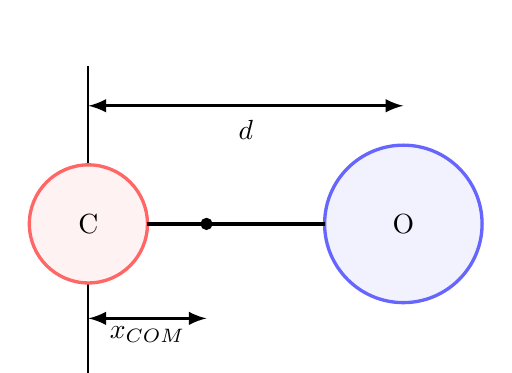
\begin{tikzpicture}[]
            \draw[black, thick] (0,4) -- (0,0);
            \filldraw[color=red!60, fill=red!5, very thick](0,2) circle (0.75);
            \filldraw[color=blue!60, fill=blue!5, very thick](4,2) circle (1);
            \draw[black, ultra thick] (0.75,2) -- (3,2);
            \filldraw [black] (1.5,2) circle (2pt);
            \node[black] at (0,2)  {C};
            \node[black] at (4,2) {O};
            \draw[black,very thick, <->] (0, 0.8) -- (1.5,0.8);
            \draw[black, very thick, <->] (0,3.5) -- (4, 3.5);
            \node[black] at (2, 3.2) {$d$};
            \node[black] at (0.75, 0.6) {$x_{COM}$};
        \end{tikzpicture}
        }
        \caption{A diatomic molecule}
        \label{fig:diatomic}
    \end{wrapfigure}
    Consider a diatomic molecule. When working on the rotational degrees of freedom, we will use two parameters: The position of the centre of mass $x_{COM}$ and the moment of inertia of the molecule around the center of mass $I_{COM}$. The position of the centre of mass is given by $x_{COM} = \frac{m_O}{m}d$ where $m$ is the total mass of the system: $m = m_O + m_C$. The moment of inertia is calculated as\\
    \begin{align}
        I_{COM} =& m_O(d-x_{COM})^2+m_Cx_{COM}^2 = m_O\lrp{d-\frac{m_Od}{m}}^2+m_C\lrp{\frac{m_Od}{m}}^2 \notag \\
        =& m_Od^2\lrp{\frac{m-m_O}{m}}^2+\frac{m_Cm_O^2d^2}{m^2} = \frac{m_Om_C^2d^2}{m^2}+\frac{m_Cm_O^2d^2}{m^2}\notag \\
        =& \frac{m_Cm_Od^2(m_O+m_C)}{m^2} = \frac{m_Cm_O}{m}d^2 = \mu d^2
    \end{align}
    where we defined the reduced mass $\mu = \frac{m_Cm_O}{m}$. From this, we can calculate the rotational energy: $L^2/2I$. Translating this into quantum mechanical variables, we get $\hat{H} = \frac{\hat{L}^2}{2I}$.
    The eigenfunctions of the squared angular momentum operator are the spherical harmonics $Y_l^m$ with eigenvalues $\varepsilon_l = \frac{\hbar^2 l(l+1)}{2I}$ with $(2l+1)$-fold degeneracy. Then the partition function is:
    \begin{equation}
        Z = \sum_l(2l+1)\exp\lrp{-\beta\frac{\hbar^2l(l+1)}{2I}}.
    \end{equation}
    Now, let us consider the limits: \\
    $T\to0\implies\beta\to\infty$: As $\beta\to0$, the exponential will decay to 0. Then we can truncate the sum at some $l$. Let us take only to $l=1$ and get $Z = 1 + 3\exp\lrp{-\frac{\hbar^2}{k_BTI}}$.
    Calculating the thermodynamical quantities:
    \begin{equation}
        F = -k_BT\ln Z = -k_BT\ln\lrp{1+3e^{-\hbar^2/k_BTI}} \approx -3k_BTe^{-\hbar^2/k_BTI}
    \end{equation}
    \begin{equation}
        S = -\periv{F}{T} = 3k_Be^{-\hbar^2/k_BTI} + 3k_BTe^{-\hbar^2/k_BTI}\lrp{\frac{\hbar^2}{k_BIT^2}} = 3k_Be^{-\hbar^2/k_BTI}\lrp{1+\frac{\hbar^2}{k_BTI}}
    \end{equation}
    \begin{align}
        C_V =& T\periv{S}{T} = 3k_BT\lrp{\frac{\hbar^2}{k_BT^2I}e^{-\hbar^2/k_BTI}\lrp{1+\frac{\hbar^2}{k_BTI}}-\frac{\hbar^2}{k_BT^2I}e^{-\hbar^2/k_BTI}}\notag\\
        =& \frac{3\hbar^4}{k_BI^2T^2}e^{-\hbar^2/k_BTI}
    \end{align}
    Now consider the $T\to\infty$ limit. Since the partition function will vary slowly at lower $l$, we can convert the sum into an integral.
    \begin{equation}
        Z\approx\int_0^\infty dl(2l+1)\exp\lrp{-\frac{\hbar^2l(l+1)}{2Ik_BT}} =\frac{2Ik_BT}{\hbar^2}=AT
    \end{equation}
    Then the free energy, entropy, and the heat capacity are
    \begin{equation}
        F = -k_BT\ln AT \implies S=k_B\ln AT + k_B \implies C_V = \frac{k_B}{T}.
    \end{equation}
    \begin{figure}[h!]
        \centering
        \resizebox{0.35\textwidth}{!}{%
        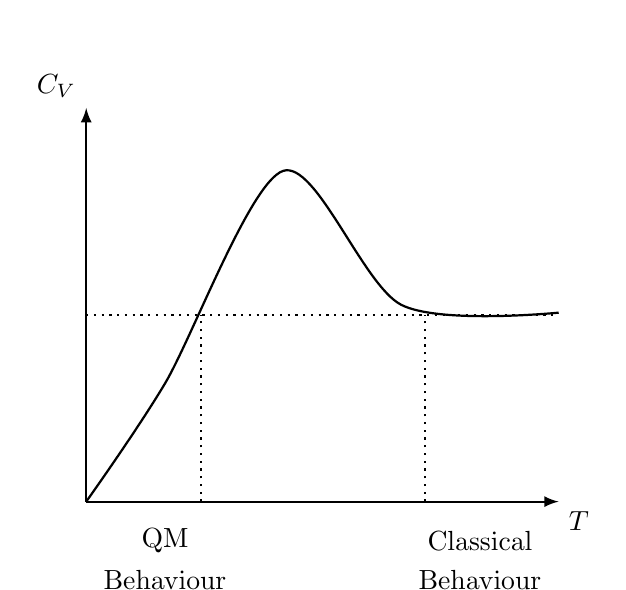
\begin{tikzpicture}
    % Axes
        \draw[thick,->] (0,0) -- (6,0) node[anchor=north west] {$T$};
        \draw[thick,->] (0,0) -- (0,5) node[anchor=south east] {$C_V$};
    
        % Horizontal dotted line
        \draw[dotted, thick] (0,2.37) -- (6,2.37);
        
        % Curve
        \draw[thick] plot[smooth] coordinates {(0,0) (1,1.5) (2.5,4.2) (4,2.5) (6,2.4)};
        
        % Dotted vertical lines
        \draw[dotted, thick] (1.46,0) -- (1.46,2.37);
        \draw[dotted, thick] (4.3,0) -- (4.3,2.37);
        
        % Labels
        \node at (1,-0.5) {QM};
        \node at (1,-1) {Behaviour};
        \node at (5,-0.5) {Classical};
        \node at (5,-1) {Behaviour};
        \end{tikzpicture}
        }
        \caption{$C_V$ plot showing the quantum mechanical and classical regions}
        \label{fig:cvrot}
    \end{figure}
    
    Now, we look at the vibrational degrees of freedom. For the vibrational motion, we observe a harmonic oscillator behaviour. The quantum mechanical harmonic oscillator has energies
    \begin{equation}
        \varepsilon_n = \hbar\omega(n+1/2).
    \end{equation}
    Therefore, the partition function is
    \begin{equation}
        Z = e^{-\hbar\omega\beta/2}\sum_{n=0}^\infty e^{\hbar\omega\beta n} = e^{-\hbar\omega\beta/2}\sum_{n=0}^\infty \lrp{e^{\hbar\omega\beta}}^n.
    \end{equation}
    This is a geometric series converging to
    \begin{equation}
        Z = \frac{e^{-\hbar\omega\beta/2}}{1-e^{\hbar\omega\beta}}.
    \end{equation}
    We again look at the low and high temperature limits:\\
    At low temperatures, the heat capacity is exactly
    \begin{equation}
        C_V=k_b(\hbar\omega\beta)^2\frac{e^{\hbar\omega\beta}}{(e^{\hbar\omega\beta}-1)^2}
    \end{equation}
    which at low temperature (high $\beta$) limit gives
    \begin{equation}
        C_V=k_B\frac{\hbar\omega\beta}{e^{\hbar\omega\beta}}.
    \end{equation}
    At high temperatures, $\hbar\omega\beta<<1$. Then,
    \begin{align}
        Z =& \frac{1}{e^{\hbar\omega\beta/2}-e^{-\hbar\omega\beta/2}}=\frac{1}{1+\frac{\hbar\omega\beta}{2}-1+\frac{\hbar\omega\beta}{2}} = \frac{k_BT}{\hbar\omega}, \\
        F =& -k_BT\ln\frac{k_BT}{\hbar\omega} = -k_BT\ln AT, \\
        S =& k_B\ln AT + k_B, \\
        C_V =& k_B.
    \end{align}
    Therefore, the total heat capacity is
    \begin{equation}
        C_V=\frac{3}{2}Nk_B + Nk_B + Nk_B.
    \end{equation}
    One must note that these degrees of freedom do not activate simultaneously. Initially (at low temperature), we only have translational degrees of freedom as the effects from the rotational and vibrational degrees of freedom die out. Then, the rotational effects are activated. At high temperatures, we have the total contribution. The activation temperatures in the case of the heat capacity are
    \begin{equation}
        T_{\mathrm{rot}} \approx \frac{\hbar^2}{2Ik_B} \hspace{0.5cm}\mathrm{and}\hspace{0.5cm}T_\mathrm{vib}\approx\frac{\hbar\omega}{k_B}
    \end{equation}
    Now, a question is: How does one calculate the partition function for continuous energy spectra, i.e. the classical limit?
    \subsection{Phase Space Representation}
        Recall that the Hamiltonian is a function of generalised coordinates and momenta. For $N$-particles, $H=H(p^N,q^N)$. Let us assume that the phase space is divided into a coarse grid with each grid having an area $\Delta A_i = \Delta x\Delta p$. The smallest area possible is $h$ due to the Heisenberg's uncertainty principle. Then, the number of states in $\Delta A_i$ is $g_i = \Delta x\Delta p / h$. This gives the partition function as
        \begin{equation}
            Z = \sum_i\frac{\Delta x\Delta p}{h}e^{-\beta E(x_i,p_i)}.
        \end{equation}
        As $\Delta x, \Delta p\to0$, we get the continuum limit: $E(x_i,p_i)\to E(x,p)$ and $\Delta x\Delta p\to dxdp$. Then,
        \begin{equation}
            Z = \frac{1}{h}\int\int dxdp_xe^{-\beta E(x,p_x)}.
        \end{equation}
        For a single particle in three dimensions, we integrate over each degree of freedom, giving us 6 integrals. 
        \begin{equation}
            Z=\frac{1}{h^3}\underbrace{\int\cdots\int}_6 d^3rd^3pe^{-\beta E(\v{r},\v{p})}
        \end{equation}
        Similarly, for $N$-particles in three dimensions, we get $6N$-integrals.
        \begin{equation}
            Z= \frac{1}{h^{3N}}\underbrace{\int\cdots\int}_{6N} d^{3N}rd^{3N}pe^{-\beta E(\v{r}_1,...,\v{r}_N,\v{p}_1,...,\v{p}_N)}
        \end{equation}
        
\section{Equipartition Theorem}
    Consider a general energy expression $E(p,q)=aq^2+bp^2$ where $a,b\in\mathbb{R}$. 
    \begin{equation}
        Z = \frac{1}{h}\int_{-\infty}^\infty dq\int_{-\infty}^\infty dp e^{-\beta(aq^2+bp^2)}=\frac{1}{h}\int_{-\infty}^\infty dq e^{-\beta aq^2}\int_{-\infty}^\infty dpe^{-\beta bp^2}
    \end{equation}
    This is a Gaussian integral giving us $Z=\frac{\pi k_BT}{h\sqrt{ab}}$. Then for $A = \frac{\pi k_B}{h\sqrt{ab}}$,
    \begin{equation}
        F = -k_BT\ln AT \hspace{1cm} S = k_B(\ln AT+1)\hspace{1cm}C_V=k_B.
    \end{equation}
    If we set $a=0$, we need to limit the position integral to a finite range to stop the partition function from diverging. 
    \begin{equation}
        Z = \frac{1}{h}\int_{-\Delta q/2}^{\Delta q/2}dq\int_{-\infty}^\infty dp e^{-\beta bp^2}=\frac{\Delta q}{h}\sqfrac{\pi}{b\beta}
    \end{equation}
    From this, we get $C_V=k_B/2$. This observation leads to the \textbf{equipartition theorem.}
    \begin{theorem}{Equipartition Theorem}
        aEvery degree of freedom that contributes a quadratic term of position or momentum to the total energy, has an average energy of $k_BT/2$ and gives a factor of $k_B/2$ to the heat capacity.
    \end{theorem}
    One can show that the Helmholtz free energy is minimised when the temperature and volume are kept constant. To prove this, we use the second law of thermodynamics: $\delta Q / T \leq \delta S$.
    \begin{equation}
        F=U-TS \implies \delta F = \delta U - T\delta S - S\delta T = \delta Q -P \delta V -T\delta S -S\delta T
    \end{equation}
    \begin{equation}
        \implies \delta F = (\delta Q -T\delta S) - P\delta V - S\delta T
    \end{equation}
    The minimum of the term in the parenthesis is 0 as stated by the second law. Then, $\delta F$ is zero when $\delta V$ and $\delta T $ are zero. 
\newpage
\section{Exercises}
    \begin{eocproblem*}{}{Each molecule in a dilute gas has an electric dipole moment of magnitude $D$. When an electric field of intensity $\varepsilon$ along the z-axis is turned on, the Hamiltonian is \begin{equation}
        H = \frac{1}{2I}p_\theta^2+\frac{1}{2I\sin^2\theta}p_\phi^2-D\varepsilon\cos\theta.
    \end{equation}
    Calculate the partition function.}
\end{eocproblem*}
        Using the Jacobian, the volume element is $dV = drd\theta d\phi dp_rdp_\theta dp_\phi$. Since $r$ is constant, we get $dV=d\theta d\phi dp_\theta dp_\phi$. Then,
        \begin{align}
            Z =& \frac{1}{h^2}\int_{-\infty}^\infty dp_\theta e^{-\beta p_\theta^2/2I}\int_0^\pi d\theta e^{\beta D\varepsilon\cos\theta}\int_{-\infty}^\infty dp_\phi e^{-\beta p_\phi^2/2I\sin^2\theta}\int_0^{2\pi} d\phi \notag\\
            =& \sqfrac{2\pi I}{\beta}\frac{2\pi}{h^2}\sqfrac{2\pi I}{\beta}\int_0^\pi d\theta \sqrt{\sin^2\theta}e^{\beta D\varepsilon\cos\theta}.
        \end{align}
        From $0$ to $\pi$, $\sqrt{\sin^2\theta}=\sin\theta$. Then,
        \begin{equation}
            Z = \frac{4\pi^2I}{\beta h^2}\int_0^\pi d\theta \sin\theta e^{\beta D\varepsilon \cos\theta} = \frac{4\pi^2I}{\beta h^2} \int_\pi^0d(\cos\theta)e^{\beta D\varepsilon\cos\theta} = \frac{4\pi^2I}{\beta h^2} \frac{e^{\beta D\varepsilon \cos\theta}}{\beta D \varepsilon}\bigg\vert_\pi^0
        \end{equation}
        \begin{equation}
            Z = \frac{8\pi^2I}{\beta^2h^2D\varepsilon}\frac{e^{\beta D\varepsilon}-e^{-\beta D\varepsilon}}{2} = \frac{8\pi^2I}{\beta^2h^2D\varepsilon}\sinh(\beta D\varepsilon)
        \end{equation}


    \begin{eocproblem*}{5.17 from Bowley \& Sanchez}
        {
        The partition function for an interacting gas is assumed to be
        \[
        Z = \left( \frac{V - Nb}{N} \right)^N \left( \frac{mk_BT}{2\pi \hbar^2} \right)^{3N/2} e^{N^2 a^2 / V k_B T}
        \]
        where \(a\) and \(b\) are constants. Show that the pressure is of the same form as van der Waals equation. Calculate the internal energy.}
    \end{eocproblem*}
        \begin{equation}
        F = U - TS = -k_B T \ln Z
        \end{equation}
        \begin{equation}
        dF = dU - TdS - SdT = TdS - PdV - TdS - SdT = -PdV - SdT
        \end{equation}
        \begin{equation}
        P = - \left( \frac{\partial F}{\partial V} \right)_T , S = - \left( \frac{\partial F}{\partial T} \right)_V
        \end{equation}
        \begin{equation}
        F = -k_B T \left[ N \ln \left( \frac{V - Nb}{N} \right) + \frac{3N}{2} \ln \left( \frac{mk_B T}{2\pi \hbar^2} \right) + \frac{N^2 a^2}{V k_B T} \right]
        \end{equation}
        \begin{equation}
        F = -Nk_B T \left[ \ln (V - Nb) - \ln N + \frac{3}{2} \ln \left( \frac{mk_B }{2\pi \hbar^2} \right) + \frac{3}{2}\ln T + \frac{N a^2}{V k_B T} \right]
        \end{equation}
        \begin{equation}
        P = - \left( \frac{\partial F}{\partial V} \right)_T = \frac{Nk_B T}{V - Nb} - \frac{N^2 a^2 k_B T}{V^2 k_B T}
        \end{equation}
        which is of the form of van der Waals equation
        \begin{equation}
        \left[ P + \frac{aN^2}{V^2} \right] (V - Nb) = Nk_B T.
        \end{equation}
        \begin{equation*}
            \begin{split}
                U = F + TS =  -Nk_B T \left[ \ln (V - Nb) - \ln N + \frac{3}{2} \ln \left( \frac{mk_B }{2\pi \hbar^2} \right) + \frac{3}{2}\ln T + \frac{N a^2}{V k_B T} \right]
        \\
            +Nk_B T \left[ \ln (V - Nb) - \ln N + \frac{3}{2} \ln \left( \frac{mk_B }{2\pi \hbar^2} \right) + \frac{3}{2}\ln T\right] + N k_B \frac{3}{2}T
            \end{split}
        \end{equation*}
        \begin{equation}
            U = -\frac{N^2a^2}{V}+\frac{3}{2} Nk_B T
        \end{equation}

        \begin{eocproblem*}{5.21 from Bowley\& Sanchez}
            {By putting $\beta = 1/k_B T$, write $Z = \sum_i e^{-\beta E_i}$, and show that
            \begin{enumerate}[label=(\alph*)]
            \item \begin{equation*}
                -\left(\frac{\partial \ln Z}{\partial\beta}\right) = \sum_i p_i E_i = \Bar{U}
            \end{equation*}
            \item Consider the second derivative of $\ln Z$ with respect to $\beta$. Show that
             \begin{equation*}
                 \left(\frac{\partial^2 \ln Z}{\partial\beta^2}\right) = \sum_i E_i^2 \frac{e^{-\beta E_i}}{Z} - \left(\sum_i E_i \frac{e^{-\beta E_i}}{Z}\right)^2 =\sum_i E_i^2 p_i - \Bar{U}^2 .
            \end{equation*}
            \item Standard deviation in energy is given by:
            \begin{equation*}
                \Delta U^2=\left(\frac{\partial^2 \ln Z}{\partial\beta^2}\right).
            \end{equation*}
            \item The average internal energy of harmonic oscillator is:
            \begin{equation*}
                \Bar{U}=\frac{\hbar\omega}{2}+\frac{\hbar\omega}{e^{\hbar\omega/k_BT}-1}.
            \end{equation*}
            \item Calculate the average internal energy and the standard deviation in energy for a two-level system with energies $\varepsilon$ and $-\varepsilon$.
            \end{enumerate}
            }
        \end{eocproblem*}
            \begin{enumerate}[label=(\alph*)]
            \item \begin{equation}
                \beta =\frac{1}{k_BT}\quad,\quad F=-k_BT\ln Z =-\frac{1}{\beta}\ln\left(\sum_i e^{-\beta E_i}\right) = \Bar{U} -TS
            \end{equation}
            
            Then,
            \begin{equation}
            \frac{\partial\beta}{\partial T}  = -\beta^2 k_B = -\frac{1}{k_BT^2}.
            \end{equation}
            \begin{align}
                 S =& - \left(\frac{\partial F}{\partial T} \right)_V = \left(\frac{\partial F}{\partial \beta} \right)_V \left(\frac{\partial \beta}{\partial T} \right)_V \notag
                 \\
                 =&-\left[\frac{1}{\beta^2}\ln Z - \frac{1}{\beta} \left(\frac{\partial \ln Z}{\partial \beta} \right) \right] (-\beta^2 k_B)\notag 
                 \\
                 =& k_B \ln Z -\beta k_B \left(\frac{\partial \ln Z}{\partial \beta} \right)
            \end{align}
            
            \begin{equation}
                F=\Bar{U}-TS \quad \implies \quad \Bar{U} = F+TS 
            \end{equation}
            \begin{equation}
            \Bar{U} = -k_BT\ln Z +T\left[k_B \ln Z -\beta k_B \left(\frac{\partial \ln Z}{\partial\beta} \right)\right]
            \end{equation}
            
            \begin{equation}
                \Bar{U} = -\left(\frac{\partial \ln Z}{\partial\beta} \right)=\sum_i p_i E_i
            \end{equation}
            
            or,
            \begin{equation}
            \begin{split}
            \left(\frac{\partial \ln Z}{\partial\beta} \right)=\frac{\partial}{\partial\beta}\ln\sum_i e^{-\beta E_i} = \frac{\sum_i -E_i e^{-\beta E_i}}{\sum_j -e^{-\beta E_j}}
            \\
            =\frac{\sum_i -E_i e^{-\beta E_i}}{Z} = =\sum_i\frac{ -E_i e^{-\beta E_i}}{Z} = -\sum_i p_i E_i = -\Bar{U}
            \end{split}
            \end{equation}
            \item 
            \begin{equation*}
                \frac{\partial^2}{\partial \beta^2} \ln Z = \frac{\partial^2}{\partial \beta^2} \ln \sum_i e^{-\beta E_i} = \frac{\partial}{\partial \beta} \left[\frac{\sum_i -E_i e^{-\beta E_i}}{\sum_i e^{-\beta E_i}}\right] 
                    \end{equation*}
                    \begin{equation}      
                    = -\frac{\partial}{\partial  \beta} \sum_i p_i E_i = -\sum_i \frac{\partial p_i}{\partial \beta}E_i - \sum_i p_i \frac{\partial E_i}{\partial \beta} = -\sum_i E_i \frac{\partial}{\partial \beta} \left(\frac{e^{\beta E_i}}{Z}\right)
                    \end{equation}
                    \begin{equation*}
                    = -\sum_i E_i e^{\beta E_i} \frac{-E_i Z-\frac{\partial Z}{\partial \beta}}{Z} = \sum_i E_i e^{\beta E_i} \frac{1}{Z}+\sum_i E_i e^{\beta E_i} \frac{1}{Z^2}\frac{\partial Z}{\partial \beta}
            \end{equation*}
            \begin{equation*}
                \frac{\partial Z}{\partial \beta} = - \sum_i E_i e^{-\beta E_i}
            \end{equation*}
            \begin{equation}  
                =\sum_i E_i^2 p_i - \underbrace{
                \sum_i E_i^2 \underbrace{
                \left(\frac{e^{-\beta E_i}}{z} \right)^2
                }_{p_i^2}
                }_{\Bar{U}^2} = \sum_i E_i^2 p_i - \Bar{U}^2
            \end{equation}
            \item \begin{equation}
                \Delta U^2 = \langle U^2 \rangle-\langle U \rangle^2
            \end{equation}
            \begin{equation}
                \Bar{U}=\langle U\rangle \quad \implies \quad \Bar{U}^2 =\sum_i E_i^2p_i
            \end{equation}
            Thus, we showed that $\frac{\partial^2 \ln Z}{\partial \beta^2} = \Bar{U^2}-\Bar{U}=\Delta U^2$.
            
            \item For a harmonic oscillator, $E_n = \left(n+\frac{1}{2}\right)\hbar\omega$.
            \begin{equation}
                Z = \sum_n e^{-\beta E_n} = \left[\sum_n (e^{-\beta\hbar\omega})^n \right] e^{-\beta\hbar\omega / 2}
            \end{equation}
            Taking $|e^{\beta\hbar\omega}|<1$, we can expand $Z$ as a geometric series.
            \begin{equation}
                Z = \frac{e^{-\beta\hbar\omega/2}}{1-e^{-\beta\hbar\omega}}
            \end{equation}
            Since $\Bar{U}=-\frac{\partial \ln Z}{\partial \beta}$ has $\ln Z$ dependence,
            \begin{equation}
                \ln Z = -\frac{\hbar\omega\beta}{2}-\ln (1-e^{-\beta\hbar\omega}).
            \end{equation}
            \begin{equation}
            \Bar{U}=\frac{\hbar\omega}{2}-\frac{\hbar\omega e^{-\beta \hbar\omega}}{1-e^{-\beta \hbar\omega}} = \frac{\hbar\omega}{2}+\frac{\hbar\omega}{e^{\hbar\omega/k_BT}-1}
            \end{equation}
            
            \item \begin{equation}
                Z=\sum_n e^{-\beta E_n}=e^{-\beta e}+e^{\beta e}
            \end{equation}
            \begin{equation}
                \begin{split}
                    \Bar{U}=-\frac{\partial \ln Z}{\partial \beta} =-\frac{\partial}{\partial \beta} \ln (e^{-\beta e}+e^{\beta e}) 
                    \\
                    =-\frac{\partial}{\partial \beta} \ln (2 \cosh \beta \varepsilon) = -\frac{\partial}{\partial \beta} (\ln 2 + \ln \cosh \beta \varepsilon)
                    \\
                    =-\frac{\varepsilon \sinh \beta \varepsilon}{\cosh \beta \varepsilon} = -\varepsilon\tanh\beta\varepsilon
                \end{split}
            \end{equation}
            Also,
            \begin{equation}
                    \Delta U^2 = \frac{\partial^2 \ln Z}{\partial \beta^2} = \frac{\varepsilon^2 \cosh^2\beta\varepsilon-\varepsilon^2\sinh^2\beta\varepsilon}{\cosh^2\beta\varepsilon} = \varepsilon^2(1-\tanh^2\beta\varepsilon)
            \end{equation}
            \end{enumerate}

\chapter{Identical Particles}

In classical mechanics and the macroscopic systems, one can distinguish any particle from another by looking at its properties. However, particles in quantum mechanical systems cannot be distinguished by their size, shape or location as they lack these properties. To demonstrate this consider a collision event between two particles of the same kind and draw a box around the collision point as demonstrated in Figure (\ref{fig:identicalcollision}).

\begin{figure}[h!]
    \centering
    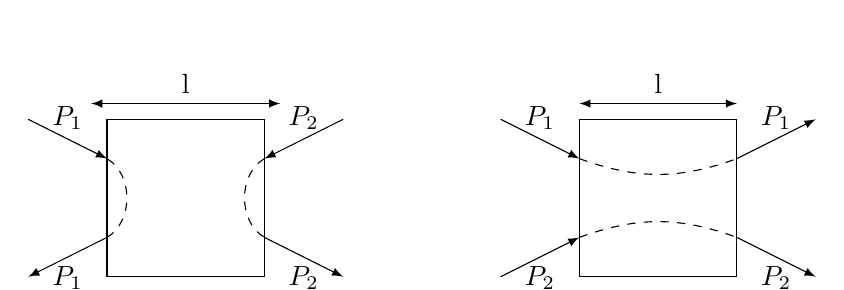
\begin{tikzpicture}
       % First diagram on the left
        \draw[->] (-2,1) -- (-1,0.5) node[midway, above] {$P_1$};
        \draw[->] (-1,-0.5) -- (-2,-1)   node[midway, below] {$P_1$};
        \draw[->] (2,1) -- (1,0.5)  node[midway, above] {$P_2$};
        \draw[->] (1,-0.5) -- (2,-1) node[midway, below] {$P_2$};
        
        % Curved dashed lines inside the square
        \draw[dashed] (-1,-0.5) to[out=30,in=-30] (-1,0.5);
        \draw[dashed] (1,0.5) to[out=210, in=150] (1,-0.5);
        
        \draw (-1,1) -- (1,1) -- (1,-1) -- (-1,-1) -- cycle;
        
        \draw[<->] (-1.2,1.2) -- (1.2,1.2) node[midway, above] {l};
        
        % Second diagram on the right (same as the left)
        \draw[->] (4,1) -- (5,0.5) node[midway, above] {$P_1$};
        \draw[->] (4,-1) -- (5,-0.5) node[midway, below] {$P_2$};
        \draw[->] (7,0.5) -- (8,1) node[midway, above] {$P_1$};
        \draw[->] (7,-0.5) -- (8,-1) node[midway, below] {$P_2$};
        
        % Curved dashed lines inside the square (curved outward)
        \draw[dashed] (5,0.5) to[out=-20,in=200] (7,0.5);
        \draw[dashed] (5,-0.5) to[out=20,in=-200] (7,-0.5);
        
        
        
        \draw (5,1) -- (7,1) -- (7,-1) -- (5,-1) -- cycle;
        
        \draw[<->] (5,1.2) -- (7,1.2) node[midway, above] {l};
        
    \end{tikzpicture}
    \caption{Two possible collision events between particles of the same kind.}
    \label{fig:identicalcollision}
\end{figure}

If the size of the box is at the order of magnitude as the uncertainty in their positions, then we cannot know which of the two processes took place. In that case, the particles are said to be \textbf{indistinguishable}. \\
Now, consider a wavefunction of two particles $\psi(x_1,x_2)$ where $x_1$ and $x_2$ are composite position-spin coordinates: $x_i = (\v{r}_i,\sigma_i)$. If the two particles are indistinct, then the expectation values cannot change under an exchange of $x_1$ and $x_2$. Howver, the wavefunction itself may not be invariant. Consider the expectation value of a Hamiltonian. 
\begin{equation}
    \expval{\hat{H}} = \int dx_1dx_2\psi^*(x_1,x_2)\hat{H}(x_1,x_2)\psi(x_1,x_2) = E\int dx_1dx_2\abs{\psi(x_1,x_2)}^2
\end{equation}
Now, if we exchange the two particles, the expectation value should be the same. Moreover, since the Hamiltonian is symmetric, it will give the same eigenvalue. 
\begin{equation}
    \expval{\hat{H}} = \int dx_2dx_1\psi^*(x_2,x_1)\hat{H}(x_2,x_1)\psi(x_1,x_2)=E\int dx_2dx_1\abs{\psi(x_2,x_1)}^2
\end{equation}
Since $dx_1$ and $dx_2$ commute in the integration measure, this equality implies
\begin{equation}
    \abs{\psi(x_1,x_2)}^2 = \abs{\psi(x_2,x_1)}^2.
\end{equation}
From this equality, we can see that the two wavefunctions differ only by a phase factor.
\begin{equation}
    \psi(x_2,x_1)=e^{i\alpha}\psi(x_1,x_2)
\end{equation}
Note that for such a two-particle system, we have to obtain the original wavefunction upon doing another exchange. Then,
\begin{equation}
    \psi(x_1,x_2) = (e^{i\alpha})^2\psi(x_1,x_2)
\end{equation}
This means that there are only two possible values for $\alpha$: $\alpha=0$ and $\alpha=\pi$. These correspond to two different types of particles:
\begin{itemize}
    \item[i)] \textbf{Bosons:} Symmetric wavefunctions $\psi(x_1,x_2)=\psi(x_2,x_1)$
    \item[ii)] \textbf{Fermions}: Antisymmetric wavefunctions $\psi(x_1,x_2)=-\psi(x_2,x_1)$
\end{itemize}
\section{Bosons}
    Imagine a Helium atom with one-particle states $\phi_i(\v{r})$. Now, consider a wavefunction describing two non-interacting Helium atoms together. Assuming that $\{\phi_i(\v{r})\}$ form an orthonormal basis set, we can ansatz the wavefunction of the whole system as
    \begin{equation}
        \psi(\v{r}_1,\v{r}_2)=\phi_i(\v{r}_1)\phi_j(\v{r}_2).
    \end{equation}
    Here, we exclude the spins as the Helium atom has spin zero. This wavefunction is neither symmetric nor antisymmetric. To symmetrize it let us add a term with the particles switched.
    \begin{equation}
        \psi(\v{r}_1,\v{r}_2)=\frac{1}{\sqrt{2}}(\phi_i(\v{r}_1)\phi_j(\v{r}_2)+\phi_i(\v{r}_2)\phi_j(\v{r}_1))
    \end{equation}
    We can furhter consider a three-particle state. 
    \begin{equation}
        \psi(\v{r}_1,\v{r}_2,\v{r}_3) = \frac{1}{\sqrt{3!}}(\phi_i(\v{r}_1)\phi_j(\v{r}_2)\phi_k(\v{r}_3)+\phi_i(\v{r}_1)\phi_j(\v{r}_3)\phi_k(\v{r}_2)+...)
    \end{equation}
    For bosons, we can have multiple particles occupying the same position/orbit. This gives
    \begin{equation}
        \psi(\v{r}_1,\v{r}_2)=\phi_i(\v{r}_1)\phi_i(\v{r}_1) \implies E = 2\varepsilon_i.
    \end{equation}
    This allows us to label the wavefunctions only by the occupation numbers: How many particles occupy a single state.
    \begin{equation}
        \psi = \ket{n_1n_2n_3...}
    \end{equation}
    \begin{problem}{Find the total energy of five harmonic oscillators in a many-particle state given by the wavefunction 
    \begin{equation}
        \psi = \ket{1021}.
    \end{equation}
    }
    Recall that the energy of the harmonic oscillator was
    \begin{equation}
        \varepsilon_n = \lrp{n+\frac{1}{2}}\hbar\omega.
    \end{equation}
    Then, $\varepsilon_0=\hbar\omega/2$, $\varepsilon_1=0$ $\varepsilon_2=5\hbar\omega/2$, and $\varepsilon_3 = 7\hbar\omega/2$. This gives us
    \begin{equation}
        E = \frac{\hbar\omega}{2} + \frac{5\hbar\omega}{2} + \frac{7\hbar\omega}{2} = 9\hbar\omega.
    \end{equation}
    \end{problem}
\section{Fermions}
    For fermions, the wavefunction is antisymmetric. Let us construct an antisymmetric wavefunction for two particles as we did in a similar way before. 
    \begin{equation}
        \psi(\v{r}_1,\v{r}_2) = \frac{1}{\sqrt{2}}(\phi_i(\v{r}_1)\phi_j(\v{r}_2)-\phi_i(\v{r}_2)\phi_j(\v{r}_1))
    \end{equation}
    Note that, this construction looks like a determinant.
    \begin{equation}
        \psi(\v{r}_1,\v{r}_2)=\frac{1}{\sqrt{2}}\begin{vmatrix}
            \phi_i(\v{r}_1) & \phi_j(\v{r}_1) \\ 
            \phi_i(\v{r}_2) & \phi_j(\v{r}_2)
        \end{vmatrix}
    \end{equation}
    For three particles, we get
    \begin{equation}
        \psi(\v{r}_1,\v{r}_2,\v{r}_3) = \frac{1}{\sqrt{6}}\begin{vmatrix}
            \phi_i(\v{r}_1) & \phi_j(\v{r}_1) & \phi_k(\v{r}_1) \\ 
            \phi_i(\v{r}_2) & \phi_j(\v{r}_2) & \phi_k(\v{r}_2) \\ 
            \phi_i(\v{r}_3) & \phi_j(\v{r}_3) & \phi_k(\v{r}_3)
        \end{vmatrix}
    \end{equation}
    Unlike bosons, if two fermions occupy the same state, then the determinant and thus the wavefunction becomes zero. This means that the probability of multiple particles occupying the same state is zero. This is the \textbf{Pauli exclusion principle}. We can still label the wavefunction by the occupation numbers but these numbers can only be 0 or 1. \\
    With this construction of wavefunction, we can generalise the energy of both the fermions and bosons as
    \begin{equation}
        E = \sum_in_i\varepsilon_i \hspace{0.5cm}\mathrm{where}\hspace{0.5cm}\sum_in_i=N.
    \end{equation}
\newpage
\section{Partition Function}
    Let us now imagine a two-particle system with three energy levels. Considering that the particles are bosons, all possible two-particle states are: 
    \begin{figure}[h!]
        \centering
        \resizebox{0.9\textwidth}{!}{%
        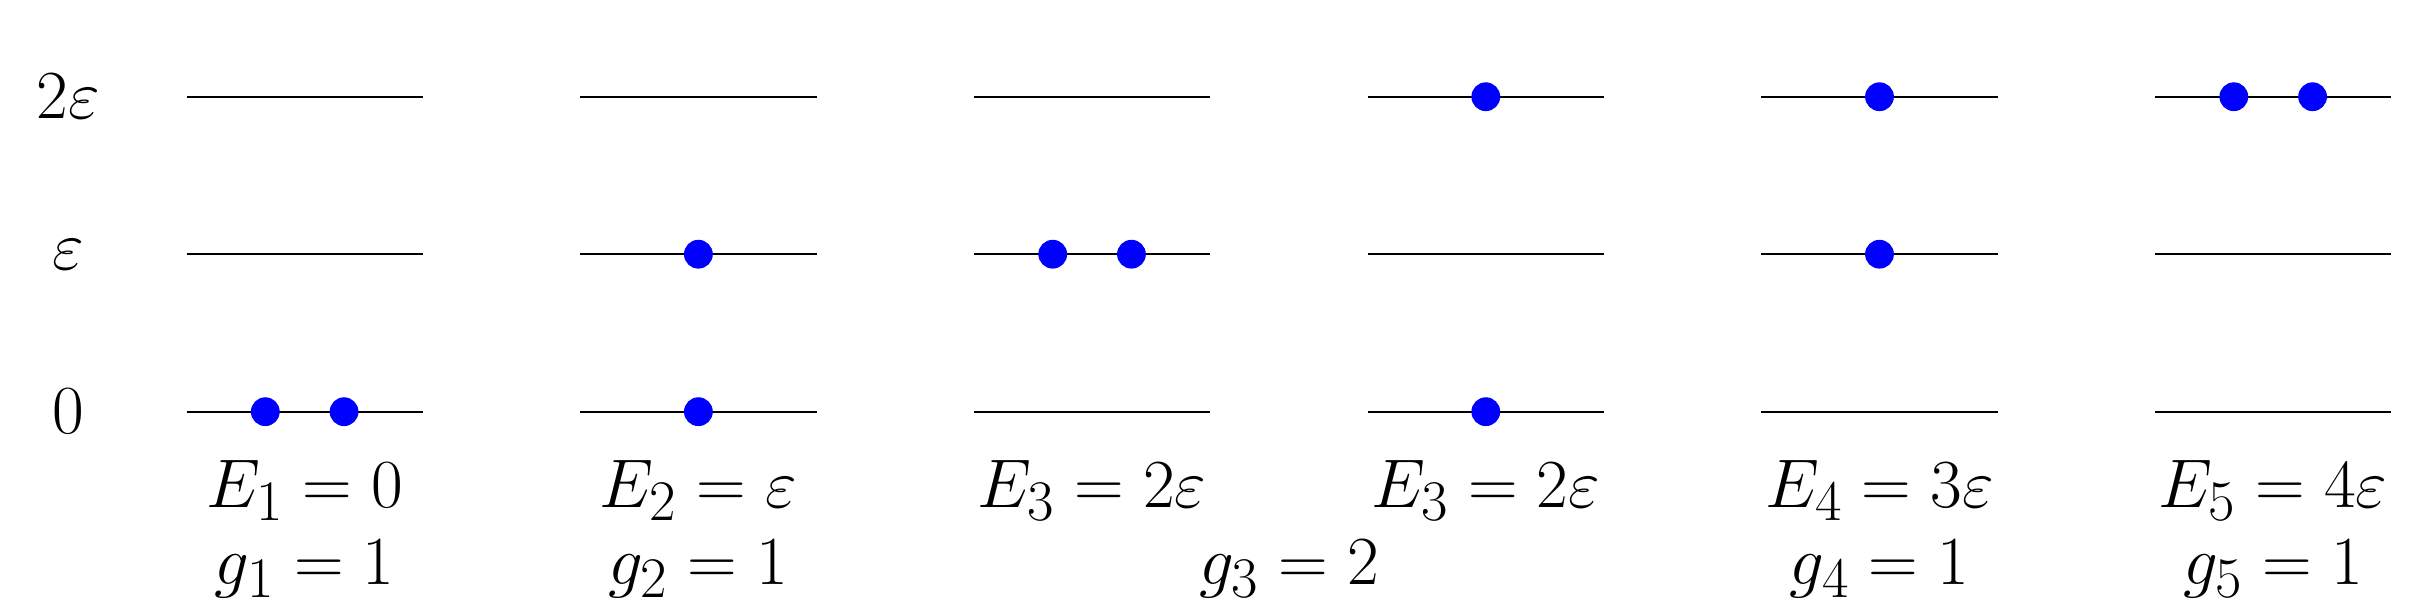
\begin{tikzpicture}
            \draw[black,thick] (0,0) -- (3,0);
            \draw[black,thick] (5,0) -- (8,0);
            \draw[black,thick] (10,0) -- (13,0);
            \draw[black,thick] (15,0) -- (18,0);
            \draw[black,thick] (20,0) -- (23,0);
            \draw[black,thick] (25,0) -- (28,0);
            \draw[black,thick] (0,2) -- (3,2);
            \draw[black,thick] (5,2) -- (8,2);
            \draw[black,thick] (10,2) -- (13,2);
            \draw[black,thick] (15,2) -- (18,2);
            \draw[black,thick] (20,2) -- (23,2);
            \draw[black,thick] (25,2) -- (28,2);
            \draw[black,thick] (0,4) -- (3,4);
            \draw[black,thick] (5,4) -- (8,4);
            \draw[black,thick] (10,4) -- (13,4);
            \draw[black,thick] (15,4) -- (18,4);
            \draw[black,thick] (20,4) -- (23,4);
            \draw[black,thick] (25,4) -- (28,4);
            \node[black,thick] at(-1.5,0) {\Huge$0$};
            \node[black,thick] at(-1.5,2) {\Huge$\varepsilon$};
            \node[black,thick] at(-1.5,4) {\Huge$2\varepsilon$};
            \node[black,thick] at(1.5, -1) {\Huge$E_1 = 0$};
            \node[black,thick] at(1.5, -2) {\Huge$g_1 = 1$};
            \node[black,thick] at(6.5, -1) {\Huge$E_2 = \varepsilon$};
            \node[black,thick] at(6.5, -2) {\Huge$g_2 = 1$};
            \node[black,thick] at(11.5, -1) {\Huge$E_3 = 2\varepsilon$};
            \node[black,thick] at(16.5, -1) {\Huge$E_3=2\varepsilon$};
            \node[black,thick] at(14, -2) {\Huge$g_3 = 2$};
            \node[black,thick] at(21.5, -1) {\Huge$E_4 = 3\varepsilon$};
            \node[black,thick] at(21.5, -2) {\Huge$g_4 = 1$};
            \node[black,thick] at(26.5, -1) {\Huge$E_5 = 4\varepsilon$};
            \node[black,thick] at(26.5, -2) {\Huge$g_5 = 1$};
            \filldraw [blue] (1,0) circle (5pt);
            \filldraw [blue] (2,0) circle (5pt);
            \filldraw [blue] (11,2) circle (5pt);
            \filldraw [blue] (12,2) circle (5pt);
            \filldraw [blue] (26,4) circle (5pt);
            \filldraw [blue] (27,4) circle (5pt); 
            \filldraw [blue] (6.5, 0) circle (5pt);
            \filldraw [blue] (6.5,2) circle (5pt);
            \filldraw [blue] (16.5, 0) circle (5pt);
            \filldraw [blue] (16.5,4) circle (5pt);
            \filldraw [blue] (21.5, 2) circle (5pt);
            \filldraw [blue] (21.5, 4) circle (5pt);
        \end{tikzpicture}
        }
        \caption{Energy levels and occupations of a two-boson system with three energy levels.}
        \label{fig:bosonenergy}
    \end{figure}
    In this case, the partition function is given as
    \begin{equation}
        Z = \sum g_ne^{-\beta E_n} = 1 + e^{-\beta\varepsilon} + 2e^{-2\beta\varepsilon} + e^{-3\beta\varepsilon} + e^{-4\beta\varepsilon}.
    \end{equation}
    Similarly, if one considers fermions, the double occupation of energy levels is not allowed and we get the following.
    \begin{figure}[h!]
        \centering
        \resizebox{0.45\textwidth}{!}{%
        \begin{tikzpicture}
            \draw[black,thick] (0,0) -- (3,0);
            \draw[black,thick] (5,0) -- (8,0);
            \draw[black,thick] (10,0) -- (13,0);
            \draw[black,thick] (0,2) -- (3,2);
            \draw[black,thick] (5,2) -- (8,2);
            \draw[black,thick] (10,2) -- (13,2);
            \draw[black,thick] (0,4) -- (3,4);
            \draw[black,thick] (5,4) -- (8,4);
            \draw[black,thick] (10,4) -- (13,4);
            \node[black,thick] at(-1.5,0) {\Huge$0$};
            \node[black,thick] at(-1.5,2) {\Huge$\varepsilon$};
            \node[black,thick] at(-1.5,4) {\Huge$2\varepsilon$};
            \filldraw [blue] (1.5, 0) circle (5pt);
            \filldraw [blue] (1.5,2) circle (5pt);
            \filldraw [blue] (6.5,0) circle (5pt);
            \filldraw [blue] (6.5,4) circle (5pt);
            \filldraw [blue] (11.5, 2) circle (5pt);
            \filldraw [blue] (11.5,4) circle (5pt);
        \end{tikzpicture}
        }
        \caption{Energy levels and occupations of a two-fermion system with three energy levels}
        \label{fig:fermionenergy}
    \end{figure}
    
    In this case, the partiton function is
    \begin{equation}
        Z = e^{-\beta\varepsilon} + e^{-2\beta\varepsilon} + e^{-3\beta\varepsilon}.
    \end{equation}
    Now consider a system consisting of two distinguishable particles. 
    \begin{figure}[h!]
        \centering
        \resizebox{0.8\textwidth}{!}{%
        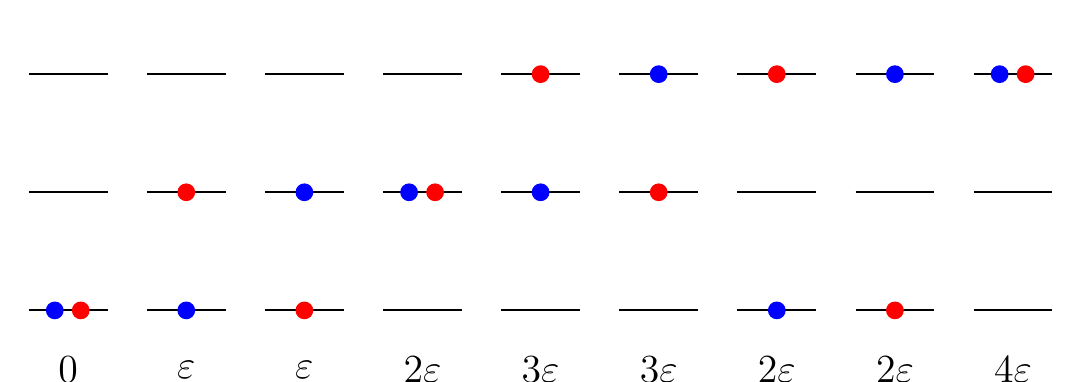
\begin{tikzpicture}
            \draw[black,thick] (0,0)--(1,0);
            \draw[black,thick] (1.5,0)--(2.5,0);
            \draw[black,thick] (3,0) -- (4,0);
            \draw[black,thick] (4.5,0) -- (5.5,0);
            \draw[black,thick] (6,0) -- (7,0);
            \draw[black,thick] (7.5, 0) -- (8.5,0);
            \draw[black,thick] (9,0) -- (10,0);
            \draw[black, thick] (10.5,0) -- (11.5,0);
            \draw[black,thick] (12,0) -- (13,0);

            \draw[black,thick] (0,1.5)--(1,1.5);
            \draw[black,thick] (1.5,1.5)--(2.5,1.5);
            \draw[black,thick] (3,1.5) -- (4,1.5);
            \draw[black,thick] (4.5,1.5) -- (5.5,1.5);
            \draw[black,thick] (6,1.5) -- (7,1.5);
            \draw[black,thick] (7.5, 1.5) -- (8.5,1.5);
            \draw[black,thick] (9,1.5) -- (10,1.5);
            \draw[black, thick] (10.5,1.5) -- (11.5,1.5);
            \draw[black,thick] (12,1.5) -- (13,1.5);

            \draw[black,thick] (0,3)--(1,3);
            \draw[black,thick] (1.5,3)--(2.5,3);
            \draw[black,thick] (3,3) -- (4,3);
            \draw[black,thick] (4.5,3) -- (5.5,3);
            \draw[black,thick] (6,3) -- (7,3);
            \draw[black,thick] (7.5, 3) -- (8.5,3);
            \draw[black,thick] (9,3) -- (10,3);
            \draw[black, thick] (10.5,3) -- (11.5,3);
            \draw[black,thick] (12,3) -- (13,3);

            \node[black, thick] at(0.5, -0.75) {\Large$0$};
            \node[black,thick] at(2, -0.75) {\Large$\varepsilon$};
            \node[black,thick] at(3.5, -0.75) {\Large$\varepsilon$};
            \node[black,thick] at(5, -0.75) {\Large$2\varepsilon$};
            \node[black,thick] at(6.5, -0.75) {\Large$3\varepsilon$};
            \node[black,thick] at(8, -0.75) {\Large$3\varepsilon$};
            \node[black,thick] at(9.5, -0.75) {\Large$2\varepsilon$};
            \node[black,thick] at(11, -0.75) {\Large$2\varepsilon$};
            \node[black,thick] at(12.5, -0.75) {\Large$4\varepsilon$};

            \filldraw [blue] (0.33,0) circle (3pt);
            \filldraw [blue] (2,0) circle (3pt);
            \filldraw [blue] (3.5,1.5) circle (3pt);
            \filldraw [blue] (4.83,1.5) circle (3pt);
            \filldraw [blue] (6.5,1.5) circle (3pt);
            \filldraw [blue] (8,3) circle (3pt);
            \filldraw [blue] (9.5,0) circle (3pt);
            \filldraw [blue] (11,3) circle (3pt);
            \filldraw [blue] (12.33,3) circle (3pt);

            \filldraw [red] (0.66,0) circle (3pt);
            \filldraw [red] (2,1.5) circle (3pt);
            \filldraw [red] (3.5,0) circle (3pt);
            \filldraw [red] (5.16,1.5) circle (3pt);
            \filldraw [red] (6.5,3) circle (3pt);
            \filldraw [red] (8,1.5) circle (3pt);
            \filldraw [red] (9.5,3) circle (3pt);
            \filldraw [red] (11,0) circle (3pt);
            \filldraw [red] (12.66,3) circle (3pt);
        \end{tikzpicture}
        }
        \caption{Energy levels and occupations of two distinguishable particles denoted with red and blue.}
        \label{fig:distinctenergies}
    \end{figure}
    \begin{equation}
        Z = 1 + 2e^{-\beta\varepsilon} + 3e^{-2\beta\varepsilon} + 2e^{-3\beta\varepsilon} + e^{-4\beta\varepsilon}
    \end{equation}
    Considering a very large number of states with $M>>N$ where $M$ is the number of states and $N$ is the number of particles. The total energy of a quantum state is $E_{ij}=\varepsilon_i+\varepsilon_j$. If $i\neq j$, then there is only one state with this energy. 
    \begin{equation}
        \psi_\alpha = \phi_i(x_1)\phi_j(x_2) \pm \phi_i(x_2)\phi_j(x_1)
    \end{equation}
    This quantum state can be written as: $ \psi_\alpha = \ket{0,0,...,1,0,0,...,1,0,0,...}$ where one particle is in the state $\phi_i(x_1)$ and the other is in $\phi_j(x_2)$. If the two particles are bosons, then we can have two particles in the same state. For example, $\psi_\beta = \phi_i(x_1)\phi_j(x_2)$ could be written as $\psi_\beta = \ket{0,0,...,2,0,0,...}$. Obviously, such a state cannot exist for fermions.\\ 
    If we have distinguishable particles, the energy is just a sum of terms involving different quantum numbers. Therefore, we can factorize the partition function. 
    \begin{equation}
        Z_2 = Z_1Z_1 = \sum_i^Me^{-\beta\varepsilon_i}\sum_j^Me^{-\beta\varepsilon_j}
    \end{equation}
    Expanding the sums,
    \begin{align}
        Z_2 =& e^{-2\beta\varepsilon_1}+e^{-2\beta\varepsilon_2}+e^{-2\beta\varepsilon_3}+...\notag\\
        & 2e^{-\beta(\varepsilon_1+\varepsilon_2)} + 2e^{-\beta(\varepsilon_1+\varepsilon_3)}+...
        \label{eq:distinguishablepartition}
    \end{align}
    Here, we see that there are two states with the energy $\varepsilon_1+\varepsilon_2$ and so on. An example of this is the $E=\varepsilon$ sections in Figure-\ref{fig:distinctenergies}. The state with this energy is counted twice. Had these particles been indistinguishable, then this would be wrong. For both the fermions and bosons, there is only one state with energy $\varepsilon_1+\varepsilon_2$. In (\ref{eq:distinguishablepartition}), there are $M^2$ terms. Now looking at the partition function for two bosons, we can have two of the particles in the same state or different states.
    \begin{equation}
        Z_\mathrm{Boson} = \sum_i^Me^{-2\beta\varepsilon_i} + \sum_{i\neq j}^Me^{-\beta(\varepsilon_i+\varepsilon_j)}
    \end{equation}
    For fermions, the first sum does not exist.
    \begin{equation}
        Z_\mathrm{Fermion} = \sum_{i\neq j}^M e^{-\beta(\varepsilon_i+\varepsilon_j)}
    \end{equation}
    Note that $Z_\mathrm{Boson}\neq Z_\mathrm{Fermion}\neq Z_1Z_1$. For bosons, there are $\frac{M^2-M}{2}+M$ terms while for fermions, there are $\frac{M^2-M}{2}$ terms. In general, for $N$ particles, there are
    \begin{equation}
        \frac{M^2-M}{N!}
    \end{equation}
    terms in the partition function. For convenience and with the assumption that $M^2>>M$ and $M^2>>N!$, we can ignore the double occupancy terms and get that for all identical particles, the partition function is
    \begin{equation}
        Z_N \approx \frac{Z_1^N}{N!}.
    \end{equation}
    \begin{problem}{Consider $N$ non-interacting particles in a box. \begin{equation}
        Z_N = \frac{Z_1^N}{N!}
    \end{equation}
    and 
    \begin{equation}
        F_1 = -k_BT\lrp{\ln V + \frac{3}{2}\ln\frac{mk_BT}{2\pi\hbar^2}}
    \end{equation}
    Find the entropy of the system.}
    a\begin{equation}
        F = -k_BT\ln Z_N = -k_BT\ln\frac{Z_1^N}{N!} = -k_BT(N\ln Z_1-\ln N!)
    \end{equation}
    From Stirling's approximation,
    \begin{equation}
        F = -k_BT\lrp{N\ln Z_1 -N\ln N + N} = -Nk_BT\ln Z_1 -Nk_BT(-\ln N + 1)
    \end{equation}
    The first term is simply $NF_1$. Then,
    \begin{align}
        F =& -Nk_BT\lrp{\ln V + \frac{3}{2}\ln\frac{mk_BT}{2\pi\hbar}-\ln N +1}\notag\\
        =& -Nk_BT\lrp{\ln\frac{V}{N}+\frac{3}{2}\ln\frac{mk_BT}{2\pi\hbar}+1}
    \end{align}
    Taking the derivative with respect to time, we obtain the entropy.
    \begin{equation}
        S = Nk_B\lrp{\ln\frac{V}{N}+\frac{3}{2}\ln\frac{mk_BT}{2\pi\hbar^2}+\frac{5}{2}}
    \end{equation}
    This is the \textbf{Sackur-Tetrode formula} for the entropy of an ideal gas. It is valid for all dilute gases at temperatures such that all vibrational or rotational modes has been frozen out. 
    \end{problem}
    

\section{Spin Degrees of Freedom}
    Remember that $x_i$ was defined as a composite cordinate $x_i=(\v{r}_i,\sigma_i)$. The spin of a particle is tightly connected to what type of particle it is. This is called the \textbf{spin-statistics theorem}.
    \begin{theorem}{Spin-Statistics Theorem}
        In unites of the reduced Planck constant $\hbar$, all particles that move in three dimensions have either an integer spin and obey Bose-Einstein statistics (i.e. they are bosons) or they have half-integer spin and obey Fermi-Dirac statistics (i.e. they are fermions).\footnote{We will get to these statistics in later chapters.}
    \end{theorem}
    The spin and space components of a state are separable if $[\v{S},\hat{H}]=0$. For a two-particle system,
    \begin{equation}
        \Psi(x_1,x_2) = \psi(\v{r}_1,\v{r}_2)\chi(\sigma_1,\sigma_2).
    \end{equation}
    Consider spin-1/2 fermions. If the spin wavefunction changes sign upon exchange of the particles, then the space function must keep the same sign, and vice versa. For spin-1/2 particles, available spin states are: $\chi_1 = \ket{\uparrow \uparrow}$, $\chi_\alpha=\ket{\uparrow, \downarrow}$, $\chi_\beta=\ket{\downarrow \uparrow}$, and $\chi_3 = \ket{\downarrow, \downarrow}$. We can also create combinations $\chi_2 = \ket{\uparrow \downarrow} + \ket{\downarrow \uparrow}$ and $\chi_4 = \ket{\uparrow\downarrow}-\ket{\downarrow \uparrow}$. Here, $\chi_1$, $\chi_2$, and $\chi_3$ are all symmetric on exchange of particles while $\chi_4$ is anti-symmetric. $\chi_\alpha$ and $\chi_\beta$ states are neither symmetric nor anti-symmetric. Looking at the total spin of these states, 
    \begin{equation}
        S^2 = S_1^2+S_2^2+2\v{S}_1\cdot\v{S}_2 \implies \begin{cases}
            S^2\chi_1 = 2\hbar^2\chi_1 \\
            S^2\chi_2 = 2\hbar^2\chi_2 \\
            S^2\chi_3 = 2\hbar^2\chi_3 \\
            S^2\chi_4 = 0
        \end{cases}
    \end{equation}
    Thus, the symmetric states form a spin triplet of states with total spin of one while the anti-symmetric state forms a spin singlet corresponding to a total spin of zero. If the total energy is $\varepsilon=\varepsilon_i+\varepsilon_j$, then the possible total states of the system are
    \begin{equation}
        \Psi(x_1,x_2)=a\underbrace{(\phi_i(\v{r_1})\phi_j(\v{r}_2)-\phi_i(\v{r}_2)\phi_j(\v{r}_1))}_\text{anti-symmetric space part}\underbrace{\begin{pmatrix}
            \ket{\uparrow\downarrow}+\ket{\downarrow\uparrow} \\
            \ket{\uparrow\uparrow}\\
            \ket{\downarrow\downarrow}
        \end{pmatrix}}_\text{symmetric spin part}
    \end{equation}
    and
    \begin{equation}
        \Psi(x_1,x_2) = b\underbrace{(\phi_i(\v{r}_1)\phi_j(\v{r}_2)+\phi_j(\v{r}_1)\phi_i(\v{r}_2))}_\text{symmetric}\underbrace{(\ket{\uparrow\downarrow}-\ket{\downarrow\uparrow})}_\text{anti-symmetric}.
    \end{equation}
    Let's use the $H_2$ molecule as an example. Consider the wavefunction of the protons. Each proton is a fermion with spin-1/2 and $\hat{H}=\hat{L}^2/2I$. The particle exchange is equivalent to a rotation by 180\textdegree. For the space part, consider only the angular momentum eigenstates. The wavefunction must change sign under exchange and therefore the total wavefunction is anti-symmetric. Let us first consider the case with the anti-symmetric spin wavefunction $(\chi_4 = \frac{1}{\sqrt{2}}(\ket{\uparrow\downarrow}-\ket{\downarrow\uparrow}))$. Then, the space wavefunction must be symmetric. Looking at the spherical harmonics,
    \begin{align*}
        Y_0^0 =& \frac{1}{2}\sqfrac{1}{\pi}\\
        Y_1^{-1} =& C_{-1}\sin\theta e^{-i\phi}\\
        Y_1^0=&C_0\cos\theta \\
        Y_1^1=&C_1\sin\theta e^{i\phi}.
    \end{align*}
    From these, only $Y_0^0$ is symmetric. A general conclusion is that odd $l$ states are anti-symmetric while even $l$ states are symmetric. Then,
    \begin{equation}
        Z = \sum_{l=\text{even}}(2l+1)e^{-\beta\hbar^2l(l+1)/2I}.
    \end{equation}
    This state is called the \textbf{parahydrogen} state. Then for a symmetric spin function, we have
    \begin{equation}
        Z = \sum_{l=\text{odd}}3(2l+1)e^{-\beta\hbar^2l(l+1)/2I}.
    \end{equation}
    This is the \textbf{orthohydrogen} state. The total partition function is the sum of orthohydrogen and parahydrogen partition functions.
    \begin{equation}
        Z = Z_\text{ortho}+Z_\text{para}
    \end{equation}
\chapter{Maxwell Distribution of Speeds}
The goal in this chapter is to find the distribution of speeds/velocities of an ideal gas at equilibrium. To start, consider the particle in a box.
\begin{equation}
    \phi_i(x,y,z) = A\sin\frac{n_1\pi x}{L_x}\sin\frac{n_2\pi y}{L_y}\sin\frac{n_3\pi z}{L_z}
\end{equation}
The eigenstates of a particle in a box can be generated from a superposition of two eigenstates of the momentum operator (with eigenvalues $\hbar k$ and $-\hbar k$). The wavevector of this state is 
\begin{equation}
    \v{k} = k_x\bas{x}+k_y\bas{y}+k_z\bas{z}
\end{equation}
where $k_i$ are defined as $n_i\pi x_i/L_i$. Thus, the wavevectors are quantized. Since $k_i$ are positive numbers, we confine $\v{k}$ to the $(+,+,+)$ octant of the $k$-space. In this case, $L_i$ can be interpreted as the dimensions of the system. If $L_i >> \lambda_D$, then the points in the space ($k$-points) are very close. Multiplying the partition function by unity, we get:
\begin{equation}
    Z=\sum e^{-\beta\varepsilon(\v{k})}=\frac{1}{\Delta k_x\Delta k_y\Delta k_z}\sum e^{-\beta\varepsilon(\v{k})}\Delta k_x\Delta k_y\Delta k_z. 
\end{equation}
At the aforementioned case, this sum becomes an integral with
\begin{equation}
    Z \approx \frac{1}{\frac{\pi}{L_x}\frac{\pi}{L_y}\frac{\pi}{L_z}}\iiint_0^\infty e^{-\beta\varepsilon(\v{k})}dk_xdk_ydk_z.
\end{equation}
The coefficient at the front is simply $V/\pi^3$. \\
Since a lot of our potentials are spherically symmetric, it is advantageous to work in spherical coordinates. Moreover, if the energy does not depend on the direction of the wavevector, then we simply get $\varepsilon(\v{k})=\varepsilon(k)$. This simplifies the triple integral over $dk_xdk_ydk_z$ into just $dk$. Here, we can define the \textbf{density of states} $D(k)$ as
\begin{equation}
    \frac{V}{\pi^3}\int d\v{k}e^{-\beta\varepsilon(\v{k})}=\int dk e^{-\beta\varepsilon(k)}D(k).
\end{equation}
We further define the number of states in a spherical shell with radius $k$ and thickness $dk$ as $dN := D(k)dk$. \\ 
\\
Let us now calculate the density of states in three, two, and one dimensions. In three dimensions, for $dV_k$ the volume of the shell and $\Delta V_k$ the volume of a box in the discretized $k$-space,
\begin{equation}
    \begin{rcases}
        \Delta V_k = \frac{\pi}{L_x}\frac{\pi}{L_y}\frac{\pi}{L_z}=\frac{\pi^3}{V}\\
        dV_k = \frac{4\pi k^2}{8}dk
    \end{rcases}dN = \frac{\frac{\pi k^2}{2}}{\frac{\pi^3}{V}}dk = \underbrace{\frac{Vk^2}{2\pi^2}}_{D(k)}dk.
\end{equation}
In two dimensions,
\begin{equation}
    \begin{rcases}
        \Delta V_k = \frac{\pi^2}{A}\\ 
        dV_k = \frac{2\pi k}{4}dk
    \end{rcases}dN = \underbrace{\frac{Ak}{2\pi}}_{D(k)}dk.
\end{equation}
And finally, in one dimensions,
\begin{equation}
    \begin{rcases}
        \Delta V_k = \frac{\pi}{L} \\ dV_k = dk
    \end{rcases}dN=\underbrace{\frac{L}{\pi}}_{D(k)}dk
\end{equation}
At this point, we can either write the partition function as a function of $k$ or as a function of $\varepsilon$. Then, we define a correspondence as
\begin{equation}
    Z = \int dk D(k)e^{-\beta\varepsilon(k)}\equiv \int d\varepsilon D(\varepsilon)e^{-\beta\varepsilon}.
\end{equation}
We also refer to $D(\varepsilon)$ as the density of states with the definition
\begin{equation}
    D(\varepsilon)d\varepsilon \equiv D(k)dk \implies D(\varepsilon)=D(k)\frac{dk}{d\varepsilon}.
\end{equation}
Note that while the form of $D(k)$ depends on the dimension of the problem, the form of $D(\varepsilon)$ depends on the functional form of $D(\varepsilon)$, i.e. $dk/d\varepsilon$.\\
\\
As an example, consider the free particle. In three dimensions, $\varepsilon=\frac{\hbar^2k^2}{2m}$. Then
\begin{equation}
    k = \sqfrac{2m\varepsilon}{\hbar^2} = \lrp{\frac{2m}{\hbar^2}}^{1/2}\varepsilon^{1/2}.
\end{equation}
\begin{equation}
    \implies \frac{dk}{d\varepsilon} = \sqrt{\frac{m}{2\hbar^2}}\varepsilon^{-1/2}
\end{equation}
Also, 
\begin{equation}
    D(k)=\frac{V}{2\pi^2}k^2 \implies D(k(\varepsilon)) = \frac{V}{2\pi^2}\frac{2m\varepsilon}{\hbar^2}.
\end{equation}
Then, by above definition,
\begin{equation}
    D(\varepsilon) = \frac{V}{\pi^2}\frac{m\varepsilon}{\hbar^2}\sqfrac{m}{2\hbar^2}\varepsilon^{-1/2} = \frac{Vm}{2\pi^2\hbar^3}\sqrt{2m\varepsilon}.
\end{equation}
In two and one dimensions,
\begin{align}
    D_2(\varepsilon) =& \frac{A}{2\pi}\frac{m}{\hbar^2}=\mathrm{constant}\\
    D_1(\varepsilon) =& \frac{L\sqrt{m}}{\sqrt{2}\pi\hbar^2}\varepsilon^{-1/2}.
\end{align}

\section{Classical Gas Velocity Distribution}
    \textbf{Question:} How many particles occupy energy states whose wavevector lies between $k$ and $k+dk$?\\
    \\
    To answer this, let us denote the number of particles as $f(k)dk$ and the number of states between $k$ and $k+dk$ as $D(k)dk$. We know that the number of occupied states is
    \begin{equation}
        N\frac{e^{-\beta\varepsilon(k)}}{Z}.
    \end{equation}
    Then, $f(k)dk = \frac{D(k)N}{Z}dk\exp\lrp{-\beta\varepsilon(k)}.$
    For the particle in a box,
    \begin{equation}
        f(k)dk = \frac{Vk^2}{2\pi^2}dk\frac{e^{-\beta\hbar^2k^2/2m}}{V/\lambda_D^3}
    \end{equation}
    \begin{equation}
        \implies f(k) = N\frac{\lambda_D^3k^2}{2\pi^2}e^{-\beta\hbar^2k^2/2m}
    \end{equation}
    Now, we convert $f(k)$ to the distribution of speeds $n(u)$.
    \begin{equation}
        n(u)du = f(k)dk \hspace{0.5cm}\mathrm{and}\hspace{0.5cm}\hbar k=mu
    \end{equation}
    \begin{equation}
        n(u)du = N\frac{\lambda_D^3u^2m^2}{2\pi^2\hbar^2}e^{-\beta mu^2/2}\frac{m}{\hbar}du
    \end{equation}
    \begin{equation}
        \therefore n(u) = \frac{\lambda_D^3m^3}{2\pi^2\hbar^3}e^{-\frac{1}{2}mu^2\beta}
    \end{equation}
    This is the \textbf{Maxwell distribution}. Since both the $f(k)$ and $n(u)$ are probability distributions, they can be used to compute averages. For any quantity $A$,
    \begin{equation}
        \bar{A} = \frac{\int dkf(k)A(k)}{\int dkf(k)} = \frac{\int dun(u)A(k(u))}{\int dun(u)}.
    \end{equation}
    As an exercise, let us calculate the average kinetic energy for an ideal gas.
    \begin{equation}
        \bar{K} = \frac{1}{2}m\bar{u}^2 = \frac{1}{2}m\frac{\int du n(u)u^2}{\int dun(u)}
    \end{equation}
    Cancelling the constants from the numerator and the denominator, we get
    \begin{equation}
        \bar{K}=\frac{1}{2}m\frac{\int du u^4e^{-mu^2\beta/2}}{\int du u^2e^{-mu^2\beta/2}}.
    \end{equation}
    Let us denote the integral in the numerator as $I_4$ and the one in the denominator as $I_2$. Defining $\alpha = m\beta/2$, 
    \begin{equation}
        I_2 = -\periv{}{\alpha}\int_0^\infty e^{-\alpha u^2}du=-\frac{1}{2}\periv{}{\alpha}\lrp{\sqfrac{\pi}{\alpha}}=\frac{\sqrt{\pi}}{4}\alpha^{-3/2}
    \end{equation}
    \begin{equation}
        I_4 = -\periv{I_2}{\alpha} = \frac{3\sqrt{\pi}}{8}\alpha^{-5/2}
    \end{equation}
    Then,
    \begin{equation}
        \bar{K} = \frac{1}{2}m\frac{\frac{3\sqrt{\pi}}{8}\alpha^{-5/2}}{\frac{\sqrt{\pi}}{4}\alpha^{-3/2}}=\frac{3m}{4\alpha} = \frac{6m}{4m\beta}
    \end{equation}
    This gives the same result we know as the kinetic theory of the ideal gas and is the same as the one we got from the equipartition theorem.
    \begin{equation}
        \bar{K} = \frac{3}{2}k_BT
    \end{equation}

\chapter{Planck's Distribution}

Goal of this chapter is to explain the behaviour of a \textbf{black body}: An object that appears black when cold, i.e. an object that absorbs all incident light. Although black bodies are by their nature black, as they absorb light, their temperature increases. This increase in temperature causes the body to glow at high temperatures. Therefore, a black body is both a perfect absorber and a perfect emitter. \\
The power emitted by a black body at temperature $T$ is given by an empirical formula. 
\begin{equation}
    \deriv{Q}{t} = A\sigma T^4
\end{equation}
Here, $A$ is the surface area of the radiating body and $\sigma$ is the \textbf{Stefan's constant}. 
\begin{equation}
    \sigma = 5.67\times 10^{-8} \si{WK^{-4}m^{-2}}
\end{equation}
This formula is called the \textbf{Stefan-Boltzmann Law}. In this chapter, we will try to understand the origin of this law. Let us begin by constructing a model for the black body.\\
\begin{enumerate}
    \item The walls absorb all incident radiation.
    \item The radiation passes through the walls but cannot escape.
    \item There is a very small hole that allows for a fraction of the radiation to escape. 
\end{enumerate}

\begin{figure}[h!]
   \centering
   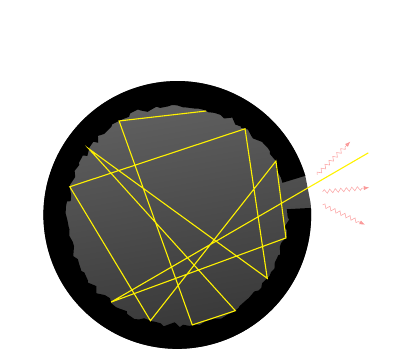
\begin{tikzpicture}[scale=1.7,rotate=10]
  
    \shade[top color=black!60,bottom color=black!80,shading angle=10] % background
      (7:1) arc (7:355:1);
    
    \fill[thick,black,postaction=decorate, % rough inner surface
      decoration={markings,mark=between positions 0.55 and 1 step 0.03 with {
                    \node[transform shape,inner sep=1pt]
                    (hit\pgfkeysvalueof{/pgf/decoration/mark info/sequence number}) {};
      }}]
      (7:1) arc (7:353:1) --++ (-7:-0.18)
      decorate[decoration={random steps,segment length=2,amplitude=1pt}]
          {arc (-7:-353:0.82)} -- cycle;
    
    \draw[yellow] % connect light ray to random points
      (8:1.5) -- (hit6.center) -- (hit1.center) -- (hit15.center) -- (hit5.center) --
      (hit9.center) -- (hit14.center) -- (hit2.center) -- (hit10.center) -- (hit3.center) --
      (hit4.center) -- (hit11.center) -- (hit13.center);
    
    \foreach \ang in {-35,-5,35}{
      \draw[radiation] (1,0)++(\ang:0.1 and 0.2) --++ (\ang:0.35);
    }
  
  \end{tikzpicture}
   \caption{A black body}
   \label{fig:blackbody}
\end{figure}

Now, we need to understand how the emitted radiation is composed in terms of differing wavelengths. Let $u(\lambda)d\lambda$ be the energy per volume in the cavity with wavelength between $\lambda$ and $\lambda+d\lambda$. Consider the energy escaping from the hole with area $A$ at an angle $\theta$ in unit time $dt$. This light wave forms a cylinder whose volume is

\begin{equation}
    dV = A'dl = A\cos\theta cdt.
\end{equation}

We now need the average power over all angles for wavelengths in this range. 

\begin{equation}
    dQ d\lambda = \frac{1}{4\pi}\int_0^{\pi/2}\int_{0}^{2\pi}(Ac\cos\theta dt)u(\lambda)d\lambda \sin\theta d\theta d\phi.     
\end{equation}
\begin{equation}
    \implies \deriv{Q}{t}d\lambda = \frac{Ac}{4\pi}u(\lambda)d\lambda\underbrace{\int_{0}^{2\pi}\cos\theta\sin\theta d\theta}_{1/2}\underbrace{\int_{0}^{2\pi}d\phi}_{2\pi} 
\end{equation}
Note that the polar angle runs only up to $\pi/2$ because we are integrating over a hemisphere. Finally, to find the total emitted power, we integrate over $\lambda$. 
\begin{equation}
    u = \int_{0}^{\infty}u(\lambda)d\lambda \implies \deriv{Q}{t} = \frac{Acu}{4}
\end{equation}
Combining this result with the Stefan-Boltzmann law,
\begin{equation}
    \frac{Acu}{4}=A\sigma T^4 \implies  u = \frac{4\sigma T^4}{c}.
\end{equation}
Next question is: How does $u(\lambda)$ look. In 19th-20th century, there have been many attempts to answer this question. We start our discussion with Wien's proposal obtained by considering classical thermodynamics only. 
\begin{equation}
    u(\lambda)d\lambda = \frac{f(\lambda T)d\lambda}{\lambda^5}
\end{equation}
Here, $f$ is an unspecified function. Let us extremise the distribution $u$. 
\begin{equation}
    \deriv{u(\lambda)}{\lambda}=\frac{f'(\lambda T)T}{\lambda^5}-\frac{5f(\lambda T)}{\lambda^6} = 0 \implies \lambda_\mathrm{max}T = \frac{5f(\lambda_mT)}{f'(\lambda_mT)}
\end{equation}
The value of the right-hand side is obtained empirically as $0.002898$. This is the \textbf{Wien's displacement law}.
\begin{equation}
    \lambda_\mathrm{max}T = 0.002898
\end{equation}
As the energy distribution, Wien proposed
\begin{equation}
    u(\lambda) = \frac{C_1e^{-C_2/\lambda T}}{\lambda^5}.
\end{equation}
As seen in Figure (\ref{fig:blackbodydist}), Wien's approximation is good at small wavelengths (high frequencies) but fails at large wavelengths (low frequencies). \\
\\
Next, we look at the Rayleigh-Jeans' proposal in the early 20th century. We assume that the cavity is a cubical box, the electromagnetic radiation is formed by standing waves and the walls are made up of charged particles acting like harmonic oscillators. The oscillators are in equilibrium with the electromagnetic wave and both have energy $k_BT$. For the electromagnetic waves, the density of states in three dimensions is
\begin{equation}
    D(k)=2\frac{L^3}{2\pi}k^2.
\end{equation}
The extra factor of 2 comes from the two polarization modes of the electromagnetic waves. We know that we can convert this into an expression in terms of $\lambda$. 

\begin{align}
    \bar{f}=\int_{0}^{\infty}f(k)D(k)dk=&\int_{\infty}^{0}f(\frac{2\pi}{\lambda})D(\frac{2\pi}{\lambda})\lrp{-\frac{2\pi}{\lambda^2}}d\lambda \notag\\
    =& \int_{0}^{\infty}f\lrp{\frac{2\pi}{\lambda}}D\lrp{\frac{2\pi}{\lambda}}\frac{2\pi}{\lambda^2}d\lambda
\end{align}

So, $D(\lambda)$ is defined as
\begin{equation}
    D(\lambda)d\lambda = 2\lrp{\frac{L^3}{2\pi^2}}\underbrace{\lrp{\frac{2\pi}{\lambda}}^2}_{k^2}\underbrace{\lrp{\frac{2\pi}{\lambda}}}_{\text{from }dk}d\lambda = \frac{8\pi L^3}{\lambda^4}d\lambda
\end{equation}

If each mode of oscillation contributes an energy of $k_BT$, then
\begin{equation}
    u(\lambda)d\lambda=D(\lambda)\frac{E(\lambda)d\lambda}{L^3}=\frac{8\pi k_BT}{\lambda^4}d\lambda
\end{equation}

Now, let us apply two criteria on $u(\lambda)$
\begin{enumerate}
    \item It satisfies the Wien's Law.
        \begin{equation}
            f(\lambda T)=8\pi k_B\lambda T \implies u(\lambda) = \frac{f(\lambda T)}{\lambda^5}
        \end{equation}
    \item The total energy is finite.
        \begin{equation}
            u = \int_{0}^{\infty}u(\lambda)d\lambda = \int_{0}^{\infty}\frac{8\pi k_BT}{\lambda^4}d\lambda \to \infty
        \end{equation}
\end{enumerate}

Therefore, we see that the Rayleigh-Jeans distribution diverges to infinity at short wavelengths and thus the total energy is not finite. Even though the long wavelength behaviour is explained nicely by the classical thermodynamics, it causes an infinite energy at short wavelengths. This, at the time, was called the \textbf{ultraviolet catastrophe}. This result was the breaking point of the classical physics that led to the creation of a new mechanics to explain the thermodynamics of black bodies. \\
\linebreak
We know look at the solution of the ultraviolet catastrophy. Put forward by Max Planck in 1900. To start, we relax the assumption that the average energy per oscillator is $k_BT$. We then propose a distribution
\begin{equation}
    u(\lambda) = \frac{8\pi hc}{\lambda^5(e^{\beta hc/\lambda}-1)}.
\end{equation}

This distribution obviously fits the Wien's law. We then have to check whether it gives a finite total energy. Let us define 
\begin{equation}
    x = \frac{hc}{\lambda k_BT} \implies dx = -\frac{hc}{k_BT}\frac{d\lambda}{\lambda^2} \hspace{0.25cm}\&\hspace{0.25cm} \lambda = \frac{hc}{xk_BT}.
\end{equation}
Then,
\begin{equation}
    \int_{0}^{\infty}u(\lambda)d\lambda = \int_{0}^{\infty}\frac{8\pi hc}{\lambda^5(e^{hc/\lambda k_BT}-1)}d\lambda \equiv I
\end{equation}
\begin{align}
    I =& \int_{0}^{\infty}8\pi hc\lrp{\frac{k_BT}{hc}}^5x^5\lrp{\frac{hc}{k_BT}}\frac{1}{x^2}\frac{1}{e^x-1}dx\notag\\
    =& 8\pi\frac{(k_BT)^4}{(hc)^3}\int_{0}^{\infty}\frac{x^3}{e^x-1}dx =  8\pi\frac{(k_BT)^4}{(hc)^3}\frac{\pi^4}{15}\notag
\end{align}
\begin{equation}
    \therefore u(\lambda) = \frac{8\pi^5k_B^4}{15h^3c^3}T^4
\end{equation}
This is finite and consistent with Stefan-Boltzmann law. Also, by maximising this distribution, one obtains the Wien's displacement law.
\begin{law*}{Wien's Displacement Law}
    As one lowers the temperature, the maximum of the emitted power shifts/displaces to lower temperatures.
    \begin{equation}
        \lambda_mT = 0.002899
    \end{equation}
\end{law*}
\begin{figure}[h!]
    \centering
    \includegraphics[width=0.5\linewidth]{wiendisplacement.png}
    \caption{The intensity vs wavelength plots, showing the Wien's displacement law.}
    \label{fig:wiendisplacement}
 \end{figure}

 Now, let us look at the origin of the Planck distribution. We start with the wave equation.
 \begin{equation}
    \frac{1}{s^2}\periv{^2y}{t^2}=\periv{^2y}{x^2}
 \end{equation}
 Solutions to this equation are either plane waves,
 \begin{equation}
    y_k(x,t) = A\sin kxe^{-i\omega t} \implies \frac{1}{s^2}\omega^2\ddot{y}_k = k^2y_K
 \end{equation}
 or harmonic oscillators with energies
 \begin{equation}
    \varepsilon_n = \lrp{n+\frac{1}{2}}\hbar\omega(k).
 \end{equation}
 The harmonic oscillator solution introduces packets of energy quantised by an integer number $n$. These quanta of energy were later named photons. The introduction of photons forms the foundation of quantum mechanics. \\
 Now we calculate the average number of particles with wavevector $\v{k}$ and energy $\hbar\omega(\v{k})$.
 \begin{equation}
    \bar{n}(\v{k}) = \sum_n^\infty np_n(\v{k})=\sum_n^\infty n\frac{e^{-n\beta\hbar\omega(\v{k})}}{Z(\v{k})}
    \label{eq:planckdist}
 \end{equation}
 Assuming isotropic distribution,
\begin{align}
    Z(k) =& 1 + \underbrace{e^{-\beta\hbar\omega}}_\text{1 photon} + \underbrace{e^{-2\hbar\omega\beta}}_\text{2 photons} + ... \notag\\
    =& \sum_n^\infty e^{-n\beta\hbar\omega(k)} = \frac{1}{1-e^{-\beta\hbar\omega(k)}}. 
    \label{eq:planckpartition}
\end{align}
Substituting (\ref{eq:planckpartition}) in (\ref{eq:planckdist}),
\begin{align}
    \bar{n} =& \sum_n^\infty ne^{-n\beta\hbar\omega(k)}\lrp{1-e^{-\beta\hbar\omega(k)}} = \lrp{1-e^{-\beta\hbar\omega(k)}}\sum_n^\infty  ne^{-n\beta\hbar\omega(k)} \notag\\
            =& -\lrp{1-e^{-\beta\hbar\omega(k)}}\periv{}{(\beta\hbar\omega)}\sum_n^\infty e^{-n\beta\hbar\omega(k)}\notag\\
            =& -\lrp{1-e^{-\beta\hbar\omega(k)}}\periv{}{(\beta\hbar\omega)}\lrp{\frac{1}{1-e^{-\beta\hbar\omega(k)}}}\notag\\
            =& (1-e^{-\beta\hbar\omega(k)})\frac{e^{-\beta\hbar\omega(k)}}{(1-e^{-\beta\hbar\omega(k)})^2} = \frac{e^{-\beta\hbar\omega(k)}}{1-e^{-\beta\hbar\omega(k)}}
\end{align}
\begin{equation}
    \therefore \bar{n}=\frac{1}{e^{\beta\hbar\omega(k)}-1}\implies \bar{u}(\v{k}) = \hbar\omega(k)\bar{n}(\v{k})
\end{equation}
Remember that, 
\begin{equation}
    u(\lambda) = D(\lambda)\frac{E(\lambda)}{V} = \frac{8\pi V}{\lambda^4}\hbar\omega(k)\frac{1}{e^{\beta\hbar\omega}-1}\frac{1}{V}.
\end{equation}
Also, $\hbar\omega(k) = \hbar ck = \hbar c\frac{2\pi}{\lambda}=\frac{hc}{\lambda}$. Putting everything together, we get the Planck distribution.
\begin{equation}
    u(\lambda) = \frac{8\pi}{\lambda^5}\frac{hc}{e^{\beta\hbar c/\lambda}-1}
\end{equation}
\begin{figure}[h!]
   \centering
   \includegraphics[width=0.5\linewidth]{blackbodydist.png}
   \caption{Three approaches to explain the black body spectra.}
   \label{fig:blackbodydist}
\end{figure}
\newpage

\section{Thermodynamics of the \\
Planck Distribution}
    The electromagnetic waves with different wavelengths in the cavity are distinguishable. Then, we can factorise the partition function. 
    \begin{equation}
        Z = Z(\v{k}_1)Z(\v{k}_2)...
    \end{equation}

    Looking at the Helmholtz free energy,
    \begin{equation}
        F = -k_BT\ln Z = -k_BT\sum_i\ln Z(\v{k}_i).
    \end{equation}
    If the distribution is isotropic, the sum can be written as the integral
    \begin{equation}
        F \approx -k_BT\int dk D(k)\ln Z(k).
    \end{equation}
    If we consider only the integral,
    \begin{equation}
        I = -2\frac{V}{2\pi^2}\int_{0}^{\infty}k^2\ln(1-e^{\beta\hbar ck})dk).
    \end{equation}
    Let us do a change of variables $x=\beta\hbar ck$ and use integration by parts.
    \begin{equation}
        I = -\frac{V}{\pi^2}\lrp{\frac{1}{\beta\hbar c}}^3\int_{0}^{\infty}x^2\ln(1-e^{-x})dx
    \end{equation}
    \begin{equation}
        \begin{rcases}
            x^2dx = dv ,\hspace{0.25cm} \frac{x^3}{3}=v\\
            u = (1-e^{-x} ),\hspace{0.25cm} du = \frac{dx}{e^x-1}
        \end{rcases} \Rightarrow I = \frac{-V}{\pi^2}\lrp{\frac{k_BT}{\hbar c}^3}\lrb{\underbrace{\lrp{\frac{x^3}{3}(1-e^{-x})}_0^\infty}_0 - \underbrace{\int_{0}^{\infty}\frac{x^3}{3}\frac{dx}{e^x-1}}_{\pi^4/15}}\notag
    \end{equation}
    \begin{equation}
         = \frac{V}{3\pi^2}\lrp{\frac{k_BT}{\hbar c}}^3\frac{\pi^4}{15}
    \end{equation}
    \begin{align}
        F =& -k_BTI=-\frac{\pi^2V}{45}\frac{(k_BT)^4}{(\hbar c)^3}\equiv -AT^4\\
        S =& -\periv{F}{T}=4AT^3\\
        P =& -\periv{F}{V}=\frac{AT^4}{V} \\
        U =& F+TS=3AT^4
    \end{align}
    Looking at the internal energy and the pressure, we see that
    \begin{equation}
        U =3PV.
    \end{equation}
    The source of this pressure is the momenta imparted by the photons on the walls of the cavity.

\section{Einstein's Model of Vibrations in Solids}
    The idea of quantization can be extended to matter waves as well as demonstrated by de Broglie in his PhD thesis. Consider the highly ordered atoms in a crystal. Let $x_i^0$ denote the positions of the lattice points of the crystal and $u_i$ the deviation of the positions of the atoms in the crystal as they vibrate. The internal energy is a function of these positions.
    \begin{equation}
        U = U(x_i^0+u_i)
    \end{equation}
    Considering the vibrations as small oscillations, we can Taylor expand this expression around the equilibrium points, i.e. the lattice points. 
    \begin{equation}
        U = U_0 +\sum_i^N \periv{U}{x_i}\bigg\vert_{x_i=x_i^0}u_i + \frac{1}{2}\sum_{i,j}^N\periv{^2U}{x_i\del x_j}u_iu_j+...
    \end{equation}
    Here, we can ignore the constant term $U_0$ and neglect the first sum. Moreover, we can define $K_{ij}=\del_i\del_jU$ to get the internal energy as a generalised harmonic oscillator.
    \begin{equation}
        U = \sum_{ij}^N\frac{1}{2}K_{ij}u_iu_j
    \end{equation}
    In this approximation, the vibration modes can be treated as quanta of energy with
    \begin{equation}
        Z = \frac{1}{1-e^{\beta\hbar\omega}}.
    \end{equation}
    Then, the free energy for N oscillators is 
    \begin{equation}
        F = k_BT\sum_\alpha \ln(1-e^{\beta\hbar\omega_\alpha})
    \end{equation}
    where we sum over all the modes of vibration. Moreover, we can add a term representing the zero point energy of the oscillations and the energy of interactions between atoms in their equilibrium positions. This gives us 
    \begin{equation}
        F = N\epsilon + k_BT\sum_\alpha \ln(1-e^{-\beta\hbar\omega_\alpha}).
        \label{eq:einsteinfreeenergy}
    \end{equation}
    \paragraph{Einstein's model of vibrations:}All modes of vibration have the same angular frequency $\omega_E$. Therefore, each mode has energy $\hbar\omega_E$. Then the sum in (\ref{eq:einsteinfreeenergy}) just gives $3Nk_BT\ln(...)$. The Helmholtz free energy is thus
    \begin{equation}
        F = N\epsilon + 3Nk_BT\ln(1-e^{-\beta\hbar\omega_E}).
        \label{eq:einsteinfreeenergy2}
    \end{equation}
    Taking the second derivative of this twice and multiplying by $(-T)$ gives us the heat capacity.
    \begin{equation}
        C_V = 3Nk_B\frac{(\beta\hbar\omega_E)^2e^{\beta\hbar\omega_E}}{(e^{\beta\hbar\omega}-1)^2}
    \end{equation}
    At high temperatures, the exponential is small. Thus, we can expand it in Taylor series. For $x=\beta\hbar\omega_E$,
    \begin{equation}
        C_V\approx ^Nk_Bx^2\frac{1+x+\frac{x^2}{2}+...}{(1+x-1)^2}\approx ^Nk_B\frac{x^2}{x^2}=3Nk_B.
    \end{equation}
    Moreover, at low temperatures, $x>>1$. 
    \begin{equation}
        C_V\approx 3Nk_Bx^2\frac{e^x}{(e^x-1)^2}=\frac{3NkBx^2e^x}{e^{2x}}=3NkB\lrp{\frac{\hbar\omega_E}{k_BT}}^2e^{-\hbar\omega_E/k_BT}
    \end{equation}
    This model fits the experiment well for high temperatures but fails at very low temperatures. 

\section{Debye's Model of Vibrations in Solids}
    Debye's model is an improvement over Einstein's model, where temperature ranges are treated separately. This helps fix the deviations of the model from the experimental data at low temperatures. At low temperatures, i.e. long wavelengths, acoustic waves are highly populated where there are many atoms per wavelength. In contrast, at hight temperatures with short wavelengths, the optical waves are populated. This proposes a wavelength dependence on the frequency of vibrations. We know this functional dependence of $\omega$ on $k$ as the \textbf{dispersion relation}. \\
    In three dimensions, for each $\lambda$, there are three modes of vibration, i.e. polarizations: Two transverse and one longitudinal mode per wavelength. \\
    For the thermodynamic properties, we start with the density of states. Since the wavevectors are discretised in exactly the same way as it was for an ideal gas, we can use the same formula for the density of states in the $k$-space. For a single polarization, 
    \begin{equation}
        D(k)dk = \frac{Vk^2dk}{2\pi^2}.
    \end{equation}
    Now, we convert the density of states to an expression in terms of the angular frequency. The transverse and longitudinal waves, in general, have different speeds for acoustic waves: $\omega_L=s_Lk$ and $\omega_T=s_Tk$. However, both are linear in wavenumber. Thus, let us derive $D(\omega)$ for a generic speed $s$. 
    \begin{equation}
        \omega = sk \implies k =\frac{\omega}{s}
    \end{equation}
    \begin{equation}
        D(\omega)=D(k(\omega))\deriv{k}{\omega}=\frac{Vk^2}{2\pi^2}\frac{1}{s}=\frac{V(\omega/s)^2}{2\pi^2s}=V\frac{\omega^2}{2\pi^2s^3}
    \end{equation}
    Now, we add all three contributions. Two from $s_T$ and one from $s_L$.\footnote{These also give the average speed of sound as $\frac{3}{\bar{s}^3}=\frac{2}{s_T^3}+\frac{1}{s_L^3}$.}
    \begin{equation}
        D(\omega) = \frac{V\omega^2}{2\pi^2}\lrp{\frac{2}{s_T^3}+\frac{1}{s_L^3}}
    \end{equation}
    In Debye's model, this density of states is used to calculate the Helmholtz free energy for acoustic waves. At low temperatures (or large frequencies), free energy is again a sum that we can write using an integral.
    \begin{equation}
        F \approx N\epsilon + \int_0^{2\pi s/\lambda_\text{min}} D(\omega)\ln(1-e^{\hbar\omega\beta})d\omega =\footnote{Since $\lambda_\text{min}\approx a$ where $a$ is a lattice constraint, it can be represented by an infinity} N\epsilon + \frac{3k_BTV}{2\pi^2\bar{s}^3}\int_{0}^{\infty}\omega^2\ln(1-e^{-\hbar\omega\beta})d\omega
    \end{equation}
    Using integration by parts and utilising the $\Gamma-$function, this integral gives
    \begin{equation}
        F = N\epsilon - \frac{\pi^2k_B^4T^4V}{30\hbar^3\bar{s}^3}
    \end{equation}
    with entropy as
    \begin{equation}
        S = \frac{2\pi^2k_B^4V}{15\hbar^3\bar{s}^3}T^3
    \end{equation}
    Now, for high temperatures (or small frequencies)
    \begin{align}
        F =& N\epsilon + k_BT\sum_\alpha \ln(1-e^{-\hbar\omega_a/k_BT})\approx N\epsilon + k_BT\sum_\alpha \ln\lrp{1-1+\frac{\hbar\omega_\alpha}{k_BT}}\notag \\
        =&N\epsilon + k_BT\sum_\alpha\ln\lrp{\frac{\hbar\omega_\alpha}{k_BT}} = N\epsilon + 3Nk_BT\ln\lrp{\frac{\hbar}{k_BT}}+k_BT\sum_\alpha\ln\omega_\alpha
    \end{align}
    We can define an average frequency by 
    \begin{equation}
        \ln\bar{\omega} = \frac{1}{3N}\sum_\alpha\ln\omega_\alpha.
    \end{equation}
    Then, 
    \begin{equation}
        F = N\epsilon + 3Nk_BT\ln\frac{\hbar}{k_BT}+3Nk_BT\ln\bar{\omega}
    \end{equation}
    Then we get $F\propto 3Nk_BT\ln AT$ which gives $C_V = 3Nk_B$. This is consistent with the equipartiton theorem. \\
    So far, we've been distinguishing the long and short wavelengths, high and low temperatures, large and small frequencies, etc. So, a natural question is: What is the cutoff frequency such that the long and short wavelengths can be distinguished? Or similarly, high temperature and low temperature? Here, we introduce the \textbf{Debye frequency} $\omega_D$ chosen so that the number of modes up to $\omega_D$ is $3N$. We then interpolate between the two regimes. 
    \begin{equation}
        3N = \int_{0}^{\omega_D}D(\omega)d\omega = \frac{3V}{2\pi^2\bar{s}^3}\int_{0}^{\omega_D}\omega^2d\omega = \frac{V\omega_D^3}{2\pi^2\bar{s}^3}
    \end{equation}
    \begin{equation}
        \implies \omega_D = \bar{s}\lrp{\frac{6N\pi^2}{V}}^{1/3}=\bar{s}\lrp{6n\pi^2}^{1/3}
    \end{equation}
    Using $\omega_D$ we can also define a \textbf{Debye energy} $\hbar\omega_D$ and a \textbf{Debye temperature} $T_D=\hbar\omega_D/k_B$. This Debye temperature is considered a border between high temperature and low temperature. In the Debye theory,
    \begin{equation}
        D(\omega)=\begin{cases}
            \frac{3V}{2\pi^2\bar{s}^3}\omega^2, & \omega<\omega_D \\
            0, & \omega>\omega_D
        \end{cases}
    \end{equation}
    Then,
    \begin{equation}
        F = N\epsilon + \frac{3k_BTV}{2\pi^2\bar{s}^3}\lrp{\frac{k_BT}{\hbar}}^3\int_{0}^{\hbar\omega_D/k_BT}x^2\ln(1-e^{-x})dx.
    \end{equation}
    As examples, the Debye temperature for Silicon is $647K$ while for Potassium, it is $89.4K$. One weak side of the Debye theory is that at very low temperatures, $C_V$ is still not consistent with the expermiental results due to electronic degrees of freedom that are not accounted by the Debye model. 
\section{Solids and Vapours in Equilibrium}
    Until now, we have seen how to calculate the partition functions for solids and gases. With this knowledge, we can look for a theory on the equilibrium between these phases knowing that at equilibrium, the Helmholtz free energy is minimised. For simplicity, we will take the gas to be Argon since it is monoatomic and spinless and use Einstein's theory for the solid. The interactions between the gas and the solid are taken to be weak so that the total partition function can be factorised into a product of the partition functions of each phases. The partition function for a solid with $N_S$ atoms can be derived from (\ref{eq:einsteinfreeenergy2}). Multiplying the first term by unity,
    \begin{align}
        F =& k_BT\beta N_S\epsilon + 3N_Sk_BT\ln(1-e^{-\beta\hbar\omega}) = k_BT\lrp{\beta N_S\epsilon + 3N_S\ln(1-e^{-\beta\hbar\omega})} \notag\\
          =& k_BT\lrp{\ln e^{\beta N_S\epsilon}+\ln(1-e^{-\beta\hbar\omega})^{3N}} = k_BT\ln\lrb{e^{\beta N_S\epsilon}(1-e^{-\beta\hbar\omega})^{3N}}
    \end{align}
    \begin{equation}
        \therefore Z_S = e^{-N_S\epsilon/k_BT}\lrp{\frac{1}{1-e^{-\hbar\omega_E/k_BT}}}^{3N}
    \end{equation}
    Here, $-\epsilon$ is the energy per atom needed to break the solid apart into seperate gas atoms and $\omega_E$ is the Einstein frequency of vibration.\\
    We know that the partition function of the gas is
    \begin{equation}
        Z_G = \frac{Z_1^{N_G}}{N_G!}
    \end{equation}
    where $Z_1$ is the single particle partition function of the gas atom. Since the gas is monoatomic and spinless, only contribution to the partition function is from the translational motion of the atoms. As we stated before, the total partition function is
    \begin{equation}
        Z = Z_GZ_S
    \end{equation}
    When an atom leaves the solid and becomes a vapour, the total number of particles does not change. Thus, $N_G+N_S$ is constant and $dN_G=-dN_S$. From the partition function, the free energy is
    \begin{equation}
        F = -k_BT\ln Z_S -k_BT\ln Z_G
    \end{equation}
    By minimising this expression as a function of $N_G$, we get
    \begin{equation}
        \periv{F}{N_G} = k_BT\periv{\ln Z_S}{N_S}-k_BT\periv{\ln Z_G}{N_G}=0.
    \end{equation}
    After some algebra, 
    \begin{equation}
        \frac{Z_1}{N_G} = \frac{e^{-\epsilon/k_BT}}{(1-e^{-\hbar\omega_E/k_BT})^3}
    \end{equation}
    By using the ideal gas law, $P=N_Gk_BT/V_G$ where $V_G$ is the volume of the gas, we get
    \begin{equation}
        P = \frac{k_BTZ_1}{V_G}e^{\epsilon/k_BT}(1-e^{-\hbar\omega_E/k_BT})^3.
    \end{equation}
    This is very crude model for the mechanics of a solid. To further improve it, we can use the Debye's model rather than Einstein's, take into account the effects of vacancies left by the atoms leaving the solid, consider a more general case with spin and take the entropy contribution into account, and include rotational and vibrational effects of a molecule into $Z_G$. 
\chapter{Systems with Variable Numbers \\ of Particles}

    In this chapter, we will look at systems where the number of particles can change. This change can occur in two ways:
    \begin{enumerate}
        \item[i)] Particles can enter or leave the system. This occurs through a permeable membrane between the two systems. If there are no external forces at work, larger density of particles in one system drives the flow of particles to the other system. In any case, the total number of particles is conserved.
        \begin{equation}
            N_A+N_B=N \implies \deriv{N_A}{N_B}=-1
        \end{equation}
        \item[ii)] A reaction occurs between the particles in a single system. This way, new kinds of particles are created from those that were already in the system. Reactions occur such that the entropy of the system increases. To satisfy this, a reaction can occur simultaneously in both directions or on one direction only. 
        \begin{equation}
            \ce{C + D <--> CD}
            \label{chem:one}
        \end{equation} 
        \begin{equation}
            N_C+N_D+N_{CD}=N \implies   \deriv{N_C}{N_D}=1 \hspace*{0.5cm} \deriv{N_C}{N_{CD}}=-1
        \end{equation}
    \end{enumerate}
    If a reaction is reversible as in the case in (\ref{chem:one}), then the reaction comes to a chemical equilibrium at some point in time. The chemical equilibrium can be reached in two ways corresponding to the two cases we mentioned before. Looking at the total entropy for the case where there is particle addition or removal, we have
    \begin{align}
        S = S_A+S_B \implies dS =& \periv{S_A}{N_A}dN_A+\periv{S_B}{N_B}dN_B \notag\\
                                =& dN_A\lrp{\periv{S_A}{N_A}-\periv{S_B}{N_B}}.
    \end{align}
    Recall that the full form of the first law was
    \begin{equation}
        dU = TdS + \mu d_N.
    \end{equation}
    If we consider that the internal energy of the systems does not change and that at equilibrium, $T_A=T_B=T$;
    \begin{equation}
        \deriv{S}{N}=-\frac{\mu}{T}
    \end{equation}
    Then,
    \begin{equation}
        dS = - \frac{N_A}{T}(\mu_A-\mu_B)
    \end{equation}
    Since the equilibrium is the state with the maximum entropy, $dS=0$. Therefore, we reach one of the equilibrium conditions.
    \begin{equation}
        \mu_A=\mu_B
    \end{equation}
    Now, we look at the reactions. For a reaction such as the one in (\ref{chem:one}),
    \begin{equation}
        S = S_C(N_C) + S_D(N_D)+S_{CD}(N_{CD})
    \end{equation}
    \begin{align}
        dS =& \periv{S_C}{N_C}dN_C + \periv{S_D}{N_D}dN_D+\periv{S_{CD}}{N_{CD}}dN_{CD}\notag\\
           =& dN_C\lrp{-\frac{\mu_C}{T_C}-\frac{\mu_D}{T_D}+\frac{\mu_{CD}}{T_{CD}}}=-\frac{dN_C}{T}(\mu_C+\mu_D-\mu_{CD})=0.
    \end{align}
    Therefore, the equilibrium condition is: $        \mu_C+\mu_D=\mu_{CD}$
    Note that if the ratio of reactants and/or products is not 1, then this ratio is reflected in the equilibrium condition.
    \begin{equation}
        \ce{O_2 + 2H_2 <-> 2H_2O} \implies \mu_{O_2} + 2\mu_{H_2}=2\mu_{H_2O}
    \end{equation}
    To generalise this: $        \sum_\text{reactants}\nu_i\mu_i = \sum_\text{products}\nu_j\mu_j$. 
    where $\nu_i$ are the stoichiometric constants.\\
    Apart from what we discussed so far, at certain cases, we might have no particle conservation condition. In that case, one of the particle numbers is independent of the others.
    \begin{equation}
        \frac{d N_B}{d N_A} = 0
    \end{equation}
    Then, at the equilibrium,
    \begin{equation}
        \frac{\del S}{\del N_A}=\frac{\del S_A}{\del N_A}+\frac{\del S_B}{\del N_B}\frac{d N_B}{d N_A}=0\implies \frac{\del S_A}{\del N_A}=-\frac{\mu_A}{T}=0.
    \end{equation}
    This is the case in black body radiation, which we will get into no further details. 
    Now let us look at what happens when the systems approach equilibrium. For particle addition/removal,
    \begin{equation}
        \frac{d S}{d T} \frac{\del S}{\del N_A}\frac{d N_A}{d t}+\frac{\del S}{\del N_B}\frac{d N_B}{d t}=\frac{d N_A}{d t}\lrp{\frac{\del S}{\del N_A}-\frac{\del S}{\del N_B}}=-\frac{d N_A}{d t}(\mu_A-\mu_B)\geq 0.
    \end{equation}
    Therefore, the number of particles on the system where the chemical potential is greater decreases as the system approaches the equilibrium. \\
    Looking at the reactions, 
    \begin{equation}
        \frac{d S}{d T} = -\frac{d N_C}{d t}\frac{\mu_C+\mu_D-\mu_{CD}}{T}\geq0
    \end{equation}
    Then if $\mu_C+\mu_D>\mu_{CD}$, the reaction will run forward and vice versa. 
    \section{Measuring and Calculating \\ the Chemical Potential}
        Recall from the first chapters that the Gibbs free energy was defined as
        \begin{equation}
            G = H-TS = U+PV_TS.
        \end{equation}
        This implies
        \begin{equation}
            dG = -SdT + VdP + \mu dN
        \end{equation}
        which can be measured expermientally. With this definition,
        \begin{equation}
            \mu = \lrp{\frac{\del G}{\del N}}_{T,P}.
        \end{equation}
        Now, since $U$ is extensive, it scales like
        \begin{equation}
            U(NS,NV)=NU(S,V).
        \end{equation}
        This, together with $U=TS-PV+\sum\mu_i N_i$ gives $G=\mu N$ via Euler's equations for homogenous functions.\footnote{See Appendix 3}. Therefore, the chemical potential is the Gibbs free energy per particle. To calculate $\mu$ we must specify the conditions. For a thermally isolated system, we know that $S=k_B\ln\Omega$. But $\Omega$ depends on $N!$. Then,
        \begin{equation}
            \mu=-T \frac{\del S}{\del N}_{U,V}=-k_BT \frac{\del \ln\Omega}{\del N}.
        \end{equation}
        Consider atoms on a lattice as an example. Each atom can be in $g$ different states with the same energy, i.e. they are $g$-fold degenerate. Then, $\Omega = g^N$. Therefore,
        \begin{equation}
            \ln\Omega = N\ln g \implies \mu = -k_BT\ln g.
        \end{equation}
        This shows that the chemical potential goes like the degeneracy of the system. \\
        Another example is an ideal gas of spin-0 atoms. Recall that 
        \begin{equation}
            S = Nk_B\lrp{\ln\frac{V}{N}+\frac{3}{2}\ln\frac{mU}{3\pi\hbar^2 N}+\frac{5}{2}}.
        \end{equation}
        \begin{equation}
            \implies \mu = -T\frac{\del S}{\del N}=-T\frac{S}{N}-Nk_BT\lrp{-\frac{N}{V}\frac{V}{N^2}-\frac{3}{2}\frac{3\pi\hbar^2N}{mU}\frac{mU}{3\pi\hbar^2 N^2}}
        \end{equation}
        \begin{equation}
            \implies \mu = -\frac{TS}{N}+k_BT+\frac{3k_BT}{2} = -k_BT\lrp{\ln\frac{V}{N}+\frac{3}{2}\ln\frac{mU}{3\pi\hbar^2N}}
        \end{equation}
        The first term is the logarithm $1/n$ where $n$ is the number density we defined before. By the definition of the internal energy from the equipartition theorem, the second term is
        \begin{equation}
            \frac{3}{2}\ln\frac{mU}{3\pi\hbar^2N}=\frac{3}{2}\ln\frac{3mNk_BT}{6\pi\hbar^2N}=\ln\lrp{\frac{mk_BT}{2\pi\hbar^2}}^{3/2}.
        \end{equation}
        This is the inverse thermal de Broglie wavelength cubed that we defined before. We now name this quantity as \textbf{quantum degeneracy} $n_Q$. Then,
        \begin{equation}
            \mu=k_BT\ln\frac{n}{n_Q}.
        \end{equation}
        At constant temperature ensemble,
        \begin{equation}
            \mu=\frac{\del F}{\del N}=-k_BT \frac{\del \ln Z}{\del N}.
        \end{equation}
        Consider a free particle with an energy offset: $\varepsilon(k)=\Delta + \frac{\hbar^2k^2}{2m}$. Then,
        \begin{equation}
            Z_1 = \sum_ke^{-\beta\varepsilon(k)} \hspace{0.5cm} Z_N = \frac{Z_1^N}{N!}.
        \end{equation}
        \begin{equation}
            F = -k_BT\ln Z_N\approx -k_BT(N\ln Z_1-N\ln N+N)=-k_BTN(\ln Z_1-\ln N+1)
        \end{equation}
        \begin{equation}
            \mu = \frac{\del F}{\del N}=-k_BT(\ln Z_1-\ln N +1-1)=-k_BT\ln\frac{Z_1}{N} = \Delta + k_BT\ln\frac{n}{n_Q}
        \end{equation}

    \section{Grand Canonical Ensemble}
        The grand canonical ensemble is an ensemble consisting of a particle and heat reservoir. In addition to constant temperature as in the canonical ensemble, the chemical potential is also constant in the grand canonical ensemble. 
        \begin{equation}\label{eq:gcetemp}
            \frac{1}{T}=k_B\lrp{\frac{\del \ln\Omega_R}{\del U_R}}_{N_R}
        \end{equation}
        \begin{equation}
            \mu = -k_BT\lrp{\frac{\del \ln\Omega_R}{\del N_R}}_{U_R}
        \end{equation}
        By integrating (\ref{eq:gcetemp}), we obtain $\Omega_R$.
        \begin{equation}
            \frac{U_R}{k_BT}=\ln\Omega_R+f(N_R)\implies \Omega_R = \alpha e^{\beta U_R+f(N_R)}
        \end{equation}
        By substituting this into the chemical potential,
        \begin{equation}
            \mu = -k_BT\lrp{\frac{\del \ln\alpha}{\del N_R}+\frac{\del }{\del N_R}(\beta U_R+f(N_R))} = -k_BT \frac{\del f}{\del N_R}
        \end{equation}
        \begin{equation}
            \implies f(N_R)=-\frac{\mu}{k_BT}N_R
        \end{equation}
        Therefore,
        \begin{equation}
            \Omega_R = \alpha e^{\beta(U_R-\mu N)}
        \end{equation}
        If the resevoir is isolated,
        \begin{equation}
            \Omega_R(U_A,N_A)=\alpha e^{\beta\lrb{(U_T-U_A)-\mu(N_T-N_A)}}=\alpha'e^{-\beta(U_A-\mu N_A)}.
        \end{equation}
        Next, imagine that system $A$ is in quantum state $i$ with wavefunction $\psi_i$. This wavefunction is both an eigenstate of $\hat{H}$ and $\hat{N}$. Then, the total number of available states to the joint system when $A$ is in state $\psi_i$ is
        \begin{equation}
            \Omega_i=\alpha'e^{-\beta(E_i-\mu N_i)}.
        \end{equation}
        For $\sum_ip_i=1$, we have
        \begin{equation}
            p_i = \frac{e^{-\beta(E_i-\mu N_i)}}{\sum_ie^{-\beta(E_i-\mu N_i)}}
        \end{equation}
        The denominator is the \textbf{grand partition function} $\Theta$.
    \section{The Grand Potential}
        We start with the definition of the entropy.
        \begin{align}
            S_M =& k_B\ln\Omega = k_B\ln\frac{M!}{n_1!n_2!...} \approx k_B\lrp{M\ln M-\sum_in_i\ln n_i} \notag\\
                =& k_B\lrp{\ln M \sum_in_i-\sum_in_i\ln n_i}= -k_BM\sum_i\frac{n_i}{M}\ln\frac{n_i}{M}
        \end{align}
        For a single system,
        \begin{equation}
            S = \frac{S_M}{M} = -k_B\sum p_i\ln p_i
        \end{equation}
        For the grand canonical ensemble,
        \begin{equation}
            S = -k_B\sum p_i\ln particles_i = -k_B\sum p_i\lrb{-(E_i-\mu N_i)\beta -\ln\Theta}
        \end{equation} 
        Using the fact that sum of the probabilities is equal to one,
        \begin{equation}
            S = \frac{\bar{U}}{T} - \frac{\mu \bar{N}}{T}+k_BT\ln\Theta
        \end{equation}
        We rearrange this equation to get the \textbf{grand potential} $\Phi_G$. 
        \begin{equation}
            \bar{U}-\mu\bar{N}-TS = -k_BT\ln\Theta = \Phi_G
        \end{equation}
        Using the grand potential, one can derive all the thermodynamics for systems with variable numbers of particles. An expression for $dS$ can be obtained by writing the entropy as a function of extensive quantitites.
        \begin{equation}
            dS = \frac{\del S}{\del U} d\bar{U} + \frac{\del S}{\del V}dV + \frac{\del S}{\del N}d\bar{N} = \frac{d\bar{U}+PdV-\mu d\bar{N}}{T}
        \end{equation}
        Hence, $d\bar{U} = -PdV +\mu d\bar{N}+TdS$. A small change in the grand potential is
        \begin{align}
            d\Phi_G =& d\bar{U} -d(\mu\bar{N})-d(TS) = -PdV +\mu d\bar{N}+TdS -\bar{N}d\mu-\mu d\bar{N}-SdT-TdS \notag\\
                    =& -PdV-\bar{N}d\mu-SdT
        \end{align}
        This equation can be used to obtain entropy, pressure, and the average number of particles.
        \begin{align}
            S =& -\lrp{\frac{\del \Phi_G}{\del T}}_{V,\mu} \\
            P =& -\lrp{\frac{\del \Phi_G}{\del V}}_{T,\mu} \\
            \bar{N}=& -\lrp{\frac{\del \Phi_G}{\del \mu}}_{T,V}
        \end{align}
    \section{Exercises}
        \begin{eocproblem*}{Section 9.8 from Bowley \& Sanchez}
            Suppose there is a surface on which there are sites where atoms can be absorbed; each site can be empty or it can have at most one absorbed atom. Let us take one site to be the system. What is the average number, $n_i$, of particles on site $i$?
        \end{eocproblem*}
        For site $i$, either there is no atom present, in which case the energy is zero, or there is one atom present with energy $\varepsilon_i$. Then the grand partition function is the sum over two states. 
        \begin{equation}
            \Theta = \sum_ie^{-\beta(E_i-\mu N_i)} = 1 + e^{-\beta(\varepsilon-\mu)}
        \end{equation}
        Therefore, the probability is
        \begin{equation}
            p_i = \frac{e^{-\beta(\varepsilon_i-\mu)}}{1+e^{-\beta(\varepsilon_i-\mu)}} = \frac{1}{e^{\beta(\varepsilon_i-\mu)}+1}.
        \end{equation}
        With this, we get the average occupation as
        \begin{equation}
            n = 0\times(1-p_i)+1\times p_i = \frac{1}{e^{\varepsilon-\mu}+1}
        \end{equation}
\chapter{Fermi and Bose Particles}
    \section{Fermions}    
        Consider the grand partition function for fermions and bosons. We start with the fermions. We will look at a system of non-interacting fermions that populate single energy states $\phi_v{k}(\v{r})$ with energy $\varepsilon(\v{k})=\varepsilon(k)$. An important distinction that we have to keep in mind is that $\varepsilon(k)$ represents the energies of the single particles while $E_i$ represents the energies of multiple-particles. Since we either have no occupence or a single occupence for a given $\v{k}$, the grand partition function is
        \begin{equation}
            \Theta(\v{k}) = \sum_ie^{-\beta(E_i-\mu)} = 1+e^{-\beta(\varepsilon(k)-\mu)}.
        \end{equation}
        This gives the grand potential as: $\Phi_G = -k_BT\ln\lrp{1+e^{-\beta(\varepsilon-\mu)}}$. \\
        Looking at a single $\v{k}$, the average number of particles in this state $\varepsilon(k)$ is
        \begin{equation}
            n(\v{k}) = -\frac{\del \Phi_G}{\del \mu} = -k_BT\frac{\beta e^{-\beta(\varepsilon-\mu)}}{1+e^{-\beta(\varepsilon-\mu)}} = \frac{1}{e^{\beta(\varepsilon(k)-\mu)}+1}.
        \end{equation}
        This is the \textbf{Fermi-Dirac Distribution}. Let us now look at the limits. Here, we need to remember that the chemical potential also depends on the temperature. As $T\to\infty$, $\mu\to-\infty$. Therefore, at high temperatures, $-\mu/k_BT>>1$ and we get $ n(\v{k}) \approx e^{-\beta(\varepsilon(k)-\mu)}$. Since the chemical potential is a positive quantity, at low temperatures, the exponent goes to zero and we get $n(\v{k})=1$. At absolute zero, the chemical potential equals the \textbf{Fermi energy}, which is the energy of the highest occupied state.
        \begin{figure}[h!]
            \centering
            \includegraphics[width=0.3\linewidth]{fermidirac.png}
            \caption{Fermi-Dirac distribution for various temperatures.}
            \label{fig:fermidirac}
        \end{figure}

        Next, let us calculate the entropy.
        \begin{equation}
            S(k) = - \frac{\del \Phi_G}{\del T} = -\frac{\del \Phi_G}{\del \beta}\frac{d\beta}{dT}=k_B\beta^2 \frac{\del \Phi_G}{\del T}
        \end{equation}
        \begin{equation}
            \frac{\del \Phi_G}{\del \beta}=\frac{1}{\beta^2}\ln(1+e^{-\beta(\varepsilon-\mu)})+ \frac{1}{\beta}\frac{\varepsilon-\mu}{e^{\beta(\varepsilon-\mu)}+1}
        \end{equation}
        \begin{equation}
            \therefore S(k) = k_B\ln(1+e^{-\beta(\varepsilon-\mu)})+\frac{k_B\beta(\varepsilon-\mu)}{e^{\beta(\varepsilon-\mu)}+1}
        \end{equation}
        Now looking at the Fermi-Dirac distribution,
        \begin{equation}
            n(k) = \frac{1}{e^{\beta(\varepsilon-\mu)}+1}\implies e^{\beta(\varepsilon-\mu)}=\frac{1}{n}-1=\frac{1-n}{n}.
        \end{equation}
        Putting this into the entropy formula,
        \begin{align}
            S(k) =& k_B\ln\lrp{1+\frac{n}{1-n}}+\frac{k_B\ln\lrp{\frac{1-n}{n}}}{\frac{1-n}{n}+1}=k_B\ln\lrp{\frac{1}{1-n}}+nk_B\ln\frac{1-n}{n} \notag\\
                =& k_B\lrb{-\ln(1-n)+n\ln(1-n)-n\ln n} = -k_B[(1-n)\ln(1-n)+n\ln n]
        \end{align}
        This is the \textbf{fermionic entropy}. If $n(k)=0$, then $S(k)=0$ also if $n(k)=1$, $S(k)=0$. Since $n(k)=1$ at absolute zero, we can say that the Fermi gas at the absolute zero of temperature has no entropy. 
    
    \section{Bosons}
        Aforementioned system with bosons instead of fermions allow all occupations. 
        \begin{equation}
            \Theta(\v{k}) = 1+e^{-\beta(\varepsilon-\mu)}+e^{-2\beta(\varepsilon-\mu)}+\dots = \sum_{n=0}^{\infty}e^{-n\beta(\varepsilon-\mu)}
        \end{equation}    
        This is a geometric series:
        \begin{equation}
            \therefore \Theta(\v{k}) = \frac{1}{1-e^{-\beta(\varepsilon-\mu)}}.
        \end{equation}
        Then the grand potential is
        \begin{equation}
            \Phi_G = -k_BT\ln\Theta(\v{k}) = \frac{1}{\beta}\ln(1-e^{-\beta(\varepsilon-\mu)}).
        \end{equation}
        In calculating these, we utilised the geometric series sum. However, for that series to be convergent, the exponential must be less than unity and therefore $\varepsilon>\mu$. We will get to the implications of this later. If we calculate the average occupation in a similar manner as we did with the fermions, we obtain the \textbf{Bose-Einstein distribution}.
        \begin{equation}
            f(\v{k})=\frac{1}{e^{\beta(\varepsilon-\mu)}-1}
        \end{equation}
        Similar to Fermi-Dirac distribution, high temperature limit gives $e^{-\beta(\varepsilon-\mu)}$. Note that this is the Maxwell-Boltzmann distribution. Therefore, both the fermions and bosons obey the Maxwell-Boltzmann distribution at high temperatures. This is the classical limit of statistical thermodynamics. We will get to the low temperature limit later. The \textbf{bosonic entropy} is similar to the fermionic entropy.
        \begin{equation}
            S(k) = k_B[(1+f)\ln(1+f)-f\ln f]
        \end{equation}
        Note that if $f(k)=0$, then $S(k)=0$.

    \section{Fermi Gas}
        We start by trying to understand the behaviour of the chemical potential as a function of temperature. In that, we calculate the total number of particles, $N$, in terms of the chemical potential. 
        \begin{equation}
            N = 2\sum_v{k} e^{-\beta(\varepsilon(\v{k})-\mu)}
        \end{equation}
        Here, the factor of 2 comes from considering the spin of the fermions. As the discrete $\v{k}$ goes to $k$ in the continuum limit, we get
        \begin{equation}
            N = 2\int n(k)D(k)dk.
        \end{equation}
        In the integral, $n(k)$ are the occupied states while $D(k)dk$ are the available states. Letting $\varepsilon(k)=\frac{\hbar^2k^2}{2m}$,
        \begin{equation}
            N = 2\int_{0}^{\infty}\frac{Vk^2}{2\pi^2}\frac{1}{e^{\beta(\frac{\hbar^2k^2}{2m}-\mu)}+1}dk.
        \end{equation}
        Changing the variables as
        \begin{equation}
            x^2 \equiv \frac{\hbar^2k^2}{2mk_BT} \implies 2xdx = \frac{\hbar^2}{mk_BT}kdk\hspace{0.25cm},\hspace{0.25cm}k=\sqrt{\frac{2mk_BT}{\hbar^2}}x
        \end{equation}
        and 
        \begin{equation}
            \eta = \frac{\mu}{k_BT},
        \end{equation}
        we get
        \begin{equation}
            n = \frac{N}{V}=\frac{1}{\pi^2}\lrp{\frac{2mk_BT}{\hbar^2}}^{3/2}\int_{0}^{\infty}\frac{x^3}{e^{x^2-\eta}+1}dx.
        \end{equation}
        This integral is hard to solve and therefore we stop here and write the number density as a function of temperature. We then deal with the rest of the solution manually.
        \begin{equation}
            n = \frac{1}{\pi^2}\lrp{\frac{2mk_BT}{\hbar^2}}^{3/2}f(\eta)\implies \eta = f^{-1}\lrp{n\pi^2\lrp{\frac{\hbar^2}{2mk_BT}}^2}
        \end{equation}
        Now we look at the behaviour at absolute zero. Recall that the energy of a fermi gas at absolute zero was the Fermi energy. With this, we define the \textbf{Fermi wavevector}, $k_F$.
        \begin{equation}
            k_F = \frac{\sqrt{2mE_F}}{\hbar}
        \end{equation}
        We then find the Fermi wavevector in terms of $n=N/V$ using the constraint on $N$. For $k<k_F$, $n(k)=1$. Then,
        \begin{equation}
            N = 2\int_{0}^{\infty}n(k)D(k)dk = 2\int_{0}^{k_F}D(k)dk = \frac{2V}{2\pi^2}\int_{0}^{k_F}k^2dk = \frac{V}{\pi^2}\frac{k_F^3}{3}
        \end{equation}
        \begin{equation}
            \therefore k_F = (3n\pi^2)^{1/3}.
        \end{equation}
        Now, looking at the internal energy,
        \begin{equation}
            U = \frac{V}{\pi^2}\int_{0}^{k_F}k^2\lrp{\frac{\hbar^2k^2}{2m}}dk = \frac{V\hbar^2}{2m\pi^2}\frac{k_F^5}{5}=\underbrace{\frac{Vk_F^3}{3\pi^2}}_N\underbrace{\frac{\hbar^2k_F^2}{2m}}_{E_F}\frac{3}{5}=\frac{3N}{5}E_F
        \end{equation}
        So far, we considered only $\Phi_G(\v{k})$. To get the total grand potential, we integrate over $v{k}$.
        \begin{equation}
            \Phi_G = -\frac{Vk_BT}{\pi^2}\int_{0}^{\infty}k^2\ln(1+e^{-\beta(\varepsilon(k)-\mu)})dk = -\frac{Vk_BT}{\pi^2}\int_{0}^{\infty}k^2\ln(1+e^{-\beta(\frac{\hbar^2k^2}{2m}-\mu)})dk
        \end{equation}
        To reduce this integral to a familiar form, we use integration by parts. 
        \begin{equation}
            x^2 = \frac{\hbar^2k^2}{2m}\beta\implies k=\sqfrac{2mk_BT}{\hbar^2}x \hspace{0.25cm},\hspace{0.25cm} dk = \sqfrac{2mk_BT}{\hbar^2}dx
        \end{equation}
        \begin{equation}
            I = \lrp{\frac{2mk_BT}{\hbar^2}}^{3/2}\int x^2\ln(1+e^{-(x^2-\eta)})dx
        \end{equation}
        \begin{align}
            u = \ln(1+e^{-(x^2-\eta)}) \hspace{0.5cm}& du=\frac{-2xe^{-(x^2-\eta)}}{1+e^{-(x^2-\eta)}}=\frac{-2x}{e^{x^2-\eta}+1} \\
            dv = x^2dx \hspace{0.5cm}& v =\frac{x^3}{3}
        \end{align}
        \begin{equation}
            I = \bigg(\cdots\bigg)^{3/2}\lrb{\underbrace{\lrp{\frac{x^3}{3}\ln(1+e^{-(x^2-\eta)})}_0^\infty}_0+ \frac{2}{3}\int_{0}^{\infty}\frac{x^4}{e^{x^2-\eta}+1}dx}
        \end{equation}
        The pressure of the Fermi gas in terms of the total grand potential is
        \begin{equation}
            P = \frac{\Phi_G}{V}.
        \end{equation}
        Then, we get
        \begin{equation}
            P = \frac{2k_BT}{3\pi^2}\lrp{\frac{2mk_BT}{\hbar^2}}^{3/2}\int_{0}^{\infty}\frac{x^4}{e^{x^2-\eta}+1}dx.
        \end{equation}
        Now, let us see if we can derive an equivalent form of the ideal gas law. Starting from the density of particles and doing the same change of variables as before,
        \begin{equation}
            n = \frac{N}{V} = \frac{1}{V}\int_{0}^{\infty}D(k)n(k)dk = \frac{1}{\pi^2}\int_{0}^{\infty}\frac{k^2dk}{e^{\beta(\varepsilon-\mu)}+1}
        \end{equation}
        \begin{equation}
            n = \frac{1}{\pi^2}\lrp{\frac{2mk_BT}{\hbar^2}}^{3/2}\int_{0}^{\infty}\frac{x^2dx}{e^{x^2-\eta}+1}
        \end{equation}
        Combining this with the pressure expresion,
        \begin{equation}
            \frac{P}{nk_BT}=\frac{2}{3}\frac{\int_{0}^{\infty}\frac{x^4dx}{e^{x^2-\eta}+1}}{\int_{0}^{\infty}\frac{x^2dx}{e^{x^2-\eta}+1}}=\frac{2}{3}\frac{\frac{3}{8}\sqrt{\pi}}{\frac{1}{4}\sqrt{\pi}}=1 \implies PV = Nk_BT
        \end{equation}
        At absolute zero, we go back to the original expression.
        \begin{equation}
            P = \frac{k_BT}{\pi^2}\int_{0}^{\infty}k^2\ln(1+e^{-\beta(\varepsilon-\mu)})dk 
        \end{equation}
        Doing integration by parts,
        \begin{align}
            du = k^2 dk \hspace{0.5cm}& u = \frac{k^3}{3}\\
            v = \ln\lrp{1+e^{-\beta\lrp{\frac{\hbar^2k^2}{2m}-\mu}}} \hspace*{0.5cm}& dv = -\frac{\beta\hbar k}{m}\frac{e^{-\beta(\dots)}}{1+e^{-\beta(...)}}
        \end{align}
        The last factor in $dv$ is the Fermi-Dirac distribution which is 1 if $k<k_F$ and 0 if $k>k_F$ at absolute zero. Then,
        \begin{equation}
            P = \frac{k_BT}{\pi^2}\frac{\hbar^2}{mk_BT}\frac{1}{3}\int_{0}^{k_F}k^4dk = \frac{\hbar^2k_F^5}{15m\pi^2}=\frac{2}{5}\frac{\hbar^2k_F^2}{2m}\frac{k_F^3}{3\pi^2}
        \end{equation}
        \begin{equation}
            \therefore P = \frac{2nE_F}{5}
        \end{equation}
        This means that we have finite pressure at absolute zero. \\
        Finally, let us look at the low temperature behaviour of the Fermi gas. Defining the \textbf{Fermi temperature}, $T_F$, via $k_BT_F=E_F$; for temperature lower than the Fermi temperature, the gas is degenerate. The heat capacity at temperatures lower than the Fermi temperature is
        \begin{equation}
            C_V = \frac{Nk_B\pi^2}{2}\frac{k_BT}{E_F}.
        \end{equation}
        
    \section{Non-Interacting Bose Gas}
        While working with bosons, we will index over the energies rather than states since multiple particles can occupy the same state. We begin by defining a quantity called \textbf{fugacity}, $z=e^{\beta\mu}$. With fugacity, the average particle number is 
        \begin{equation}
            \expval{N} = \sum_\varepsilon\expval{n_\varepsilon} = \sum_\varepsilon\frac{1}{z^{-1}e^{\beta\varepsilon}-1}.
        \end{equation}
        We can convert this to an integral via
        \begin{equation}
            \expval{N} = \int D(\varepsilon)f(\varepsilon)d\varepsilon = \frac{Vm\sqrt{2m}}{2\pi^2\hbar^3}\int\frac{\sqrt{\varepsilon}}{z^{-1}e^{\beta\varepsilon}-1}d\varepsilon.
        \end{equation}
        However, note that $\varepsilon=0$ in the integral gives zero while it is nonzero in the sum. Therefore, we add $\varepsilon=0$ term by hand. We keep the lower limit on the integral still at zero since the integral is continous and not discrete as the sum.
        \begin{equation}\label{eq:bosestar}
            N = \frac{2\pi}{h^3}(2m)^{3/2}V\int_{0}^{\infty}\frac{\sqrt{\varepsilon}d\varepsilon}{z^{-1}e^{\beta\varepsilon}-1}+ \frac{z}{1-z}
        \end{equation}
        Let us make a change of variables and look at the integral only. 
        \begin{equation}
            x = \beta\varepsilon \implies I  = \int_{0}^{\infty}\frac{\sqrt{k_BTx}}{z^{-1}e^x-1}k_BTdx
        \end{equation}
        Placing this into (\ref{eq:bosestar}) and defining $N_0 = z/(1-z)$, 
        \begin{equation}
            \frac{N-N_0}{V} = \frac{2\pi}{h^3}(2mk_BT)^{3/2}\int_{0}^{\infty}\frac{\sqrt{x}dx}{z^{-1}e^x-1}=\frac{2}{\sqrt{\pi}}\frac{1}{\lambda_D^3}\int_{0}^{\infty}\frac{\sqrt{x}dx}{z^{-1}e^x-1}.
        \end{equation}
        To calculate this integral we define \textbf{Bose-Einstein Functions} as
        \begin{equation}
            g_\nu(z)=\frac{1}{\Gamma(\nu)}\int_{0}^{\infty}\frac{x^{\nu-1}dx}{z^{-1}e^x-1},
        \end{equation}
        where $\Gamma(\nu)$ is the gamma function. In our case, we have $g_{3/2}(z)$ with $\Gamma\lrp{\frac{3}{2}}=\frac{\sqrt{\pi}}{2}$. Then,
        \begin{equation}
            \frac{N-N_0}{V}=\frac{g_{3/2}(z)}{\lambda_D^3} =: \frac{N_e}{V}.
        \end{equation}
        Looking at the second term in (\ref{eq:bosestar}), 
        \begin{equation}
            N_0 = \frac{z}{1-z}\implies z = \frac{N_0}{1+N_0}.
        \end{equation}
        Therefore, $0\leq z \leq 1$. Then, when fugacity takes its maximum value, i.e. 1;
        \begin{equation}
            N_e = \frac{V}{\lambda_D^3}g_{3/2}(1).
        \end{equation}
        This value of the Bose-Einstein function is equal to the Riemann zeta function of 3/2. Also, $g_{3/2}(z)$ is a monotonic function. Therefore, if $z=1$ is the maximum fugacity, 
        \begin{equation}
            g_{3/2}(z)\leq \zeta\lrp{\frac{3}{2}}
        \end{equation}
        and 
        \begin{equation}
            N_e \leq \frac{V}{\lambda_D^3}\zeta\lrp{\frac{3}{2}}.
        \end{equation}
        This puts a limit to how many particles we may have in the system. Now a question is: What happens if we add more particles? In that case, excited states will take as many particles as they can while the remaining particles will be pushed to the ground state $\varepsilon=0$.
        \begin{equation}
            N_0 = N - \frac{V}{\lambda_D^3}\zeta\lrp{\frac{3}{2}}
        \end{equation}
        The value of $z$ is now determined by
        \begin{equation}
            z = \frac{N_0}{N_0+1}\approx 1 
        \end{equation}
        for large $N_0.$ This phenomenon of a very large number of particles occupying the same ground state is called the \textbf{Bose-Einstein condensation}. The transition temperature at which a Bose-Einstein condensate begins to form is found via 
        \begin{equation}
            N_e^\mathrm{max} = V\frac{(2\pi mk_BT_c)^{3/2}}{h^3}\zeta\lrp{\frac{3}{2}}.
        \end{equation}
        For $T<T_c$, the system is a mixture of two phases:
        \begin{itemize}
            \item[-] Normal phase with $N_e$ particles 
            \item[-] Condensed phase with $N_0=N-N_e$ particles.  
        \end{itemize}
        Now, let us look at the thermodynamical variables of a Bose gas. Starting with pressure,
        \begin{equation}
            P = -\frac{\del \Phi_G}{\del V} = -\frac{\Phi_G}{V}\implies PV=k_BT\ln\Theta \implies \beta PV=\ln\Theta.
        \end{equation}
        In the case of bosons with $T>T_c$:
        \begin{equation}
            \beta P = -\int_{0}^{\infty}\ln(1-ze^{-\beta\varepsilon})\underbrace{\frac{2\pi V}{h^3}(2m)^{3/2}\sqrt{\varepsilon}}_{D(\varepsilon)}d\varepsilon.
        \end{equation}
        Changing the variables and integrating by parts gives
        \begin{equation}
            \beta P = 2\pi\lrp{\frac{\sqrt{2mk_BT}}{h}}^3\frac{2}{3}\int_{0}^{\infty}\frac{x^{3/2}dx}{ze^{-x}-1}=\frac{1}{\lambda_D^3}g_{5/2}(z).
        \end{equation}
        For $T<T_c$, fugacity goes to unity and we get
        \begin{equation}
            \frac{P}{k_BT}=\frac{1}{\lambda_D^3}\zeta\lrp{\frac{5}{2}}.
        \end{equation}
        Now, looking at the internal energy,
        \begin{equation}
            U=-\frac{\del \ln\Theta}{\del \beta}=kT^2 \frac{\del }{\del T}\lrp{\frac{PV}{k_BT}}=k_BT^2Vg_{5/2}(z) \frac{\del \lambda_D^{-3}}{\del T}
        \end{equation}
\newpage
    \section{Exercises}
        \begin{eocproblem*}{}
            Using the continuous approximation, discuss the phenomenon of the Bose-Einstein condensation and the existence of a critical temperature for one and two dimensional systems with edge length $L$. Assume $\varepsilon=p^2/2m$.
        \end{eocproblem*}
            Here we need to work through the occupation number for each dimension. Starting with two dimensions, 
            \begin{equation}
                D_2(\varepsilon) = \frac{A m}{2\pi\hbar^2}.
            \end{equation}
            \begin{equation}
                \implies \expval{N} = \int \frac{A m}{2\pi\hbar^2}\frac{1}{e^{\beta(\varepsilon-\mu)}-1}d\varepsilon
            \end{equation}
            Substituting $x=\beta\varepsilon$,
            \begin{equation}
                \expval{N} = k_BT\frac{A m}{2\pi\hbar^2}\int \frac{dx}{e^{x-\beta\mu}-1} = k_BT\frac{Am}{2\pi\hbar^2}\int\frac{dx}{z^{-1e^x-1}}
            \end{equation}
            At critical temperature, $\mu\to0$.
            \begin{equation}
                \therefore \expval{N} = k_BT_c\frac{Am}{2\pi\hbar^2}\int\frac{dx}{e^x-1} = k_BT_c\frac{Am}{2\pi\hbar^2}\zeta(1)
            \end{equation}
            Since zeta function at $x=1$ is divergent, the occupation number diverges at critical temperatures in two dimensions.\\
            Now consider one dimension. 
            \begin{equation}
                \expval{N} = \frac{L\sqrt{m}}{\sqrt{2}\pi\hbar^2}\int\varepsilon^{-1/2}\frac{d\varepsilon}{e^{\beta(\varepsilon-\mu)}-1}
            \end{equation}
            Again, substituting $x=\beta\varepsilon$,
            \begin{equation}
                \expval{N} = \frac{L\sqrt{m}}{\pi\hbar^2\sqrt{2}}\int(k_BTx)^{-1/2}\frac{k_BT dx}{e^{x-\eta}-1}.
            \end{equation} 
            \begin{equation}
                \expval{N} = \frac{L}{\pi\hbar^2}\sqfrac{mk_BT}{2}\int\frac{x^{-1/2}dx}{z^{-1}e^x-1} = \frac{L}{\pi\hbar^2}\sqfrac{mk_BT}{2}g_{1/2}(z).
            \end{equation}
            Again, at critical temperature, we get a zeta divergence. Thus in both cases $T_c=0$ and there is no Bose-Einstein condensation.
        \begin{eocproblem*}{}
            Consider a collection of $\expval{N}$ bosonic quantum harmonic oscillators in two dimensions with spin-0 and frequency $\omega$.
            \begin{enumerate}
                \item[i)] Identify the critical value of the chemical potential $\mu_c$ for which the $\expval{N}$ has a divergence.
                \item[ii)] Give an estimate for the chemical potential $\mu$ in the limit $z\to0$. 
                \item[iii)] Discuss the existence of a Bose-Einstein condensate.   
            \end{enumerate}
        \end{eocproblem*}
            \paragraph{i)}
            The average particle number for a state with quantum numbers $(n_x,n_y)$ is
            \begin{equation}
                \bar{n}(n_x,n_y) = \frac{1}{z^{-1}e^{\beta\hbar\omega(n_x+n_y+1)}-1}.
            \end{equation}
            To find the total average number of particles, we convert the double sum to a single sum: $n_x+n_y=n$. Then for each $n_x=0,...,n$ there is one $n_y=n-n_x$. This means that there are $n+1$ possible combinations. Thus, 
            \begin{equation}
                \expval{N} = \sum_{n=0}^{\infty}\frac{n+1}{z^{-1}e^{\beta\hbar\omega(n+1)}-1}.
            \end{equation} 
            For $\expval{N}$ to be divergent, $z^{-1}e^{\beta\hbar\omega(n+1)}-1$=0. Then at the ground state,
            \begin{equation}
                z_c = e^{\beta\hbar\omega} \implies \mu_c = \hbar\omega.
            \end{equation}
            \paragraph{ii)} As $z\to0$, the denominator will grop rapidly and therefore we can neglect the $-1$ term. Then, $\expval{N}$ can be approximated by
            \begin{equation}
                \expval{N} = \sum_{n_x,n_y=0}^{\infty}\frac{1}{z^{-1}e^{\beta\hbar\omega(n_x+n_y+1)}-1}\approx ze^{\beta\hbar\omega}\sum_{n_x,n_y=0}^{\infty}e^{-\beta\hbar\omega(n_x+n_y)}.
            \end{equation}
            In this case, the $n_x$ and $n_y$ are independent. Thus,
            \begin{equation}
                \expval{N} \approx ze^{\beta\hbar\omega}\lrp{\sum_{n=0}^{\infty}e^{-n\beta\hbar\omega}}^2=\frac{ze^{-\beta\hbar\omega}}{(1-e^{-\beta\hbar\omega})^2}=\frac{z}{4\sinh^2\frac{\beta\hbar\omega}{2}}.
            \end{equation}
            This gives the chemical potential as
            \begin{equation}
                \mu = \frac{1}{\beta}\ln\lrp{4\expval{N}\sinh^2\frac{\beta\hbar\omega}{2}}.
            \end{equation}
            \paragraph{iii)} The critical temperature is found by imposing $\mu\to\mu_c$, $T=T_c$, $N=0$.
            \begin{equation}
                \expval{N} = \sum_{n=1}^{\infty}\frac{n+1}{e^{n\beta_c\hbar\omega}-1}
            \end{equation}
\newpage
        \begin{eocproblem*}{}
            Compute the average number of particles for a fully degenerate relativistic gas with $s=1/2$ in a cubic container of edge length $L$. The gas is under the effect of a constant gravitational acceleration $g$ acting along one direction. Consider explicitly the cases
            \begin{enumerate}
                \item[i)] Non-relativistic: $v<<c$
                \item[ii)] Ultrarelativistic: $v\approx c$ 
            \end{enumerate}
        \end{eocproblem*}
            General expression for the momentum is
            \begin{equation}
                \v{p} = \frac{m\v{v}}{\sqrt{1-\frac{v^2}{c^2}}}
            \end{equation}
            with
            \begin{equation}
                \varepsilon_k(p) = c\sqrt{p^2+m^2c^2}.
            \end{equation}
            For non-relativistic case, the kinetic energy $\varepsilon_k = p^2/2m$ while for ultrarelativistic case $\varepsilon_k=pc$. Then, the total energies are $\varepsilon = \frac{p^2}{2m}+mgx$ and $\varepsilon=pc+mgx$ respectively. Now, we are to find $\expval{N}$ in terms of $\varepsilon_F$ at $T=0$. For the non-relativistic case,
            \begin{equation}
                \expval{N} = \frac{4\pi(2s+1)}{(2\pi\hbar)^3}L^3\int_{0}^{\sqrt{2m\varepsilon_F}}p^2dp\int_{0}^{-\frac{p^2}{2m^2g}+\frac{\varepsilon_F}{mg}}dx = \frac{L^2}{\pi^2\hbar^3}\frac{4\sqrt{2}}{15}\frac{\varepsilon_F^{5/2}\sqrt{m}}{g}.
            \end{equation}
            For the ultrarelativistic case,
            \begin{equation}
                \expval{N} = \frac{L^2}{\pi^2\hbar^3}\int_{0}^{\varepsilon_F/c}p^2dp\int_{0}^{\frac{-pc+\varepsilon_F}{mg}}dx=\frac{L^2}{\pi^2\hbar^3}\frac{\varepsilon_F^4}{12mgc^3}.
            \end{equation}
        \begin{eocproblem*}{}
            An average number $N$ of fermions is placed in a volume $V$ at temperature $T=0$. The single particle energy is $\varepsilon=\frac{p^2}{2m}$. Give an estimate for the isothermal compressibility
            \begin{equation}
                K_T = -\frac{1}{V}\lrp{\frac{\del V}{\del P}}_{T,N}.
            \end{equation}

        \end{eocproblem*}
            At $T=0$, $F=U-TS=U$. Moreover, we know that the pressure is
            \begin{equation}
                P=\frac{2n\varepsilon_F}{5}=\frac{2n}{5}\frac{5U}{3N} \implies U = \frac{3}{5}N\varepsilon_F\implies \varepsilon_F = \frac{5U}{3N}.
            \end{equation}
            Then, $PV = 2U/3$. 
            \begin{equation}
                P = -\frac{\del F}{\del V} = -\frac{\del U}{\del V} = -\frac{\del }{\del V}\lrp{\frac{2}{3}PV}=-\frac{2}{3}\lrp{V \frac{\del P}{\del V}+P}
            \end{equation}
            Evaluating the first term with $\varepsilon_F = \frac{\hbar^2k_F^2}{2m}=\frac{\hbar^2}{2m}(3\pi^2N)^{2/3}$,
            \begin{equation}
                \frac{\del P}{\del V} = \frac{\del }{\del V}\lrp{\frac{2N}{5}\frac{\hbar^2}{2m}(3\pi^2N)^{2/3}} = \frac{3\pi^2\hbar^2}{2m}\frac{2}{5} \frac{\del }{\del V}\lrp{\frac{N}{V}}^{5/3}.
            \end{equation}
            \begin{equation}
                \therefore V \frac{\del P}{\del V}=\frac{5}{3}P = \frac{10U}{9V}
            \end{equation}
            \begin{equation}
                \therefore K = -\frac{1}{V} \frac{\del V}{\del P}=\lrp{\frac{\hbar^2}{3m}(3\pi^2)^{2/3}\lrp{\frac{N}{V}^{5/3}}}^{-1}
            \end{equation}
\chapter{Phase Transitions}
    By Gibbs' definition, \textbf{phase} is a state of matter, which is uniform throughout, both in chemical and physical sense. By outside influence, phase of the system can change in a \textbf{phase transition}. Phase transition manifests itself as an abrupt change in one or more properties of the system. For example, in a material transitioning to a superconductor, the electrical resistivity goes from a finite number to zero. During the phase transition, two phases can coexist separated by a boundary. This is called the \textbf{phase separation}. 
    \section{Thermodynamic Potential}
        Consider a system of $N_A$ identical particles, placed in a heat bath with temperature $T_R$ and pressure $P_R$. The equilibrium is identified as the state which minimises the thermodynamical potential. For constant pressure and a fixed number of particles,\begin{equation}
            G = U_A + P_RV_A-T_RS_A.
        \end{equation}
        Minimising this function with respect to the internal energy and volume,
        \begin{equation}
            \frac{\del G}{\del U_A} = 1 - T_R \frac{\del S_A}{\del U_A} = 1-\frac{T_R}{T_A}.
        \end{equation}
        This is zero when $T_R=T_A$, i.e. when the temperatures of the system and the reservoir are equal. Differentiating with respect to volume,
        \begin{equation}
            \frac{\del G}{\del V_A} = P_R -T_R \frac{\del S_A}{\del V_A}=P_R-\frac{T_R}{T_A}P_A,
        \end{equation}
        which is zero when $T_A=T_R$ and $P_A=P_R$. Then, we can define the thermodynamic potential as a function of state that gets minimised under a certain set of constraints. We now define a \textbf{generalised thermodynamic potential}, $\Phi(\phi)$ where $\phi$ is a variable quantity. For example, if the thermodynamic potential is the grand potential, then $\phi = N$. To simplify, we can set that $\Phi$ depends only on the average value of $\phi$ and not the fluctuations in its value. \\
        \\
        $\Phi(\phi)$ can have one or multiple local minima. An example is water and water vapour. These are the two phases of the same material, $H_2O$, which correspond to two different minima of the potential. At low temperatures, the minima (well) corresponding to the water is more favourable. However, as temperature increases, the vapour well becomes more favourable.\\
        \\
        Consider the thermodynamic potential $\Phi(x_1,x_2,...)$ which depends on all constrained parameters, $x_i$. If any of the derivatives $\del_i\Phi$ are discontinous at the transition, then we have a \textbf{first-order transition}. If however, all derivatives are continous, we get a \textbf{second-order phase transition}. Second-order transitions are also called continous transitions. As an example, consider the Gibbs free energy. We have $x_1 =T$ and $x_2=P$. 
        \begin{equation}
            S = - \lrp{\frac{\del G}{\del T}}_P \hspace{0.5cm} V = \lrp{\frac{\del G}{\del P}}_T
        \end{equation}
        If we consider the two entropies corresponding to the two wells,
        \begin{equation}
            S_1=-lrp{\frac{\del \Phi}{\del T}}_{P,1} \hspace*{0.5cm} S_2=-\lrp{\frac{\del \Phi}{\del T}}_{P,2}.
        \end{equation}
        Here, the entropies may be different. The difference between the entropies gives the \textbf{latent heat}. For $T_p$ the transition temperature, latent heat is given by
        \begin{equation}
            L_{1,2} := T_p(S_1-S_2).
        \end{equation}
        In general, well defined boundaries exist between regions where different phases are stable. These boundaries can be seen in \textbf{phase diagrams.}
        \begin{figure}[h!]
           \centering
           \includegraphics[width=0.5\linewidth]{phasediagram.png}
           \caption{The phase diagram of the water.}
           \label{fig:phasediagram}
        \end{figure}

        On the boundary lines, the phases are equally stable. The point where all three major phases (solid, liquid, and gas) are stable is called the \textbf{triple point}. If a system crosses a boundary, then a first-order transition occurs. \\
        \\
        First-order transitions also display \textbf{metastability}. Consider a potential with two wells. Initially, well 2 is favoured. As the temperature increases, the minimum of well 2 becomes higher than that of the well 1. At that point, well 2 becomes metastable. By crossing a free-energy barrier via thermal activation, the system goes from the well 2 phase to well 1 phase. If the barrier is considerably larger than the $k_BT$ of the system, this activation can take time. However, as the system is cooled, the barrier shrinks to zero. Then, the system rapidly moves to well 1. \\
        If the barrier is sufficiently large, the metastable state persists indefinetly. Then, the metastable state seems to be a thermodynamically stable.  \\
        \\
        A liquid can be cooled below its solidification temperature and can remain a liquid until a solid is nucleated and spreads. At this state, the liquid is said to be \textbf{supercooled}. A supercooled liquid is a metastable state and this stability can last until a nucleus is formed either by further cooling or by artificially planted. \\
        The lowest temperature that a supercooled liquid can reach before the solid phase is formed is lower than the actual solidifcation temperature. If we were to take the system around a cycle in which the solid is first heated and then cooled, we would obtain two different estimates of the transition temperature. For the same temperature, we could either have a solid or a supercooled liquid depending on the point in the cycle. This behaviour is known as \textbf{hysteresis}.

        \section{Clapeyron Equation}
            If two coexisting phases are in equilibrium, i.e. $\mu_1=\mu_2$ and $G_1=G_2$ and we consider two nearby points on the phase boundary line, $(P,T)$ and $(P+dP,T+dT)$, then
            \begin{align}
                G_1(T,P) =& G_2(T,P) \\
                G_1(T+dT,P+dP) =& G_2(T+dT,P+dP)
            \end{align}
            If we expand (11.2.2) in Taylor series,
            \begin{equation}
                G_1(T,P) + \frac{\del G_1}{\del T} dT + \frac{\del G_1}{\del P}dP = G_2(T,P)+\frac{\del G_2}{\del T}dT + \frac{\del G_2}{\del P}dP.
            \end{equation}
            Rearranging gives
            \begin{equation}
                \lrp{\frac{\del G_1}{\del P}-\frac{\del G_2}{\del P}}dP = -\lrp{\frac{\del G_1}{\del T}-\frac{\del G_2}{\del T}}dT.
            \end{equation}
            From $dG = -SdT + VdP$, (11.2.4) becomes
            \begin{equation}
                \frac{dP}{dT}=-\frac{\frac{\del G_1}{\del T}-\frac{\del G_2}{\del T}}{\frac{\del G_1}{\del P}-\frac{\del G_2}{\del P}} = \frac{S_1-S_2}{V_1-V_2} = \frac{L_{12}}{T_p\Delta V}.
            \end{equation}
            This is the \textbf{Clapeyron equation}.
            \begin{equation}
                \frac{dP}{dT} = \frac{L_{12}}{T_p\Delta V}
            \end{equation}

        \section{Phase Separation}
            Consider two experiments. In one, there is a movable piston while in the other, the piston is fixed. In the first experiment, lowering the temperature will cause the volume and thus the density to change whereas in the second one, the density will remain fixed as the volume does not change. If the system cannot lower the density, then it can minimise the potential $\Phi$ via phase separation. Let $\phi$ be the fixed variable and imagine a two-well problem. \\
            Since it is fixed, the average value of $\phi$ must be constant. Let $x$ be the fraction of the system which sits in well 1. Then the fraction of the system which sits in well 2 is $1-x$. Since $\bar{\phi}$ is constant,
            \begin{equation}
                \bar{\phi} = \frac{1}{V}\int d\v{r}\phi(\v{r}) = x\phi_1 + (1-x)\phi_2.
            \end{equation}
            We can isolate $\phi_2$ from this equation to get
            \begin{equation}
                \phi_2 = \frac{\bar{\phi}-x\phi_1}{1-x}.
            \end{equation}
            Then, we can write the thermodynamic potential as
            \begin{equation}
                \Phi(\phi_1,x) = x\Phi(\phi_1)+ (1-x)\Phi\lrp{\frac{\bar{\phi}-x\phi_1}{1-x}}. 
            \end{equation}
            By varying $\phi_1$, we can minimise the potential.
            \begin{equation}
                \frac{\del \Phi}{\del \phi_1} = x\Phi'(\phi_1)-(1-x)\frac{x}{1-x}\Phi'(\phi_2)=0
            \end{equation}
            \begin{equation}
                \therefore x\Phi'(\phi_1)-x\Phi'(\phi_2)=0
            \end{equation}
            This means that the slope at $\phi_1$ is equal to the slope at $\phi_2$. We can also minimise by varying $x$.
            \begin{equation}
                \Phi(\phi_1)-\Phi(\phi_2)+(1-x)\lrp{-\frac{\phi_1}{1-x}+\frac{\bar{\phi}-x\phi_1}{(1-x)^2}}\Phi'(\phi_2)=0
            \end{equation} 
            This gives
            \begin{equation}
                \Phi'(\phi_2)=\frac{\Phi(\phi_1)-\Phi(\phi_2)}{\frac{\phi_1-\bar{\phi}}{1-x}}=\frac{\Phi(\phi_1)-\Phi(\phi_2)}{\frac{\phi_1-x\phi_1-(1-x)\phi_2}{1-x}}=\frac{\Phi(\phi_1)-\Phi(\phi_2)}{\phi_1-\phi_2}
            \end{equation}
            These two conditions can be satisfied by drawing a double tangent to the curve $\Phi(\phi)$ touching it at $\phi=\phi_1$ and $\phi=\phi_2$. This ensures that the slopes at $\phi_1$ and $\phi_2$ are equal as well as that it equals the ratio of $\Phi(\phi_1)-\Phi(\phi_2)$ to $\phi_1-\phi_2$. \\
            If the value of $\phi$ lies in the range $[\phi_1,\phi_2]$, then the system is unstable and can lower its thermodynamic potential by phase separation. 
\input{Chapters/Appendices.tex}
\newpage

%\newgeometry{top=10pt, bottom=10pt, left=5pt, right=5pt}
\addpendix{\sout{Cheat} Formula Sheet}{app:cheat}

\setlength{\columnseprule}{0.5pt}

\begin{multicols}{3}

%COL 1
\underline{\textbf{CH 1: First Law of Th.}}\\ \\
Van der Waals Gas: \\ $\theta R = \lrp{P + \frac{a}{V^2}}(V-b)$ \\ \\
Thermodynamic Functions:\\
Enthalpy(H): $H = U + PV$ \\$dH=\theta dS+VdP$ , $\periv{H}{\theta} =\periv{Q}{\theta} = C_P$ \\
Helmholtz Free Energy(F):\\ $F=U-\theta S$, $dF =-(PdV+Sd\theta)$\\
Gibbs Free Energy(G):\\ $G=U-\theta S+PV$, $dG = VdP-Sd\theta$ \\ \\
First Law: \\ $\Delta U = W+Q$ \\
(Reversible): \\ $dU = \dbar Q_{\text{rev}} -PdV$ \\ \\
For ideal gas: \\ $\Delta W = -nR\theta_G\ln\lrp{\frac{V_2}{V_1}}$ \\ $U=\frac{3}{2}nR\theta$, $C_V = \frac{3nR}{2}, C_P = \frac{5}{2}nR$   \\ \\ 
Heat capacities (Reversible): \\
$C_V = \periv{U}{\theta}$, $C_P = C_V+P\periv{V}{\theta}$ \\ \\
Ideal, reversible, adiabatic:\\
$P = CV^{-\gamma}$, $\gamma = C_P/C_V$ \\ \\
Legendre Transformation: 
\begin{equation*}
            dg = \sum_{i=1}^ru_idx_i-\sum_{i=r+1}^nx_idu_i
\end{equation*}

\columnbreak

%COL 2
\underline{\textbf{CH 2: Entropy}} \\ \\ $dS = \frac{\dbar Q}{\theta}$ \\ \\ Ideal gas: \\ $\Delta S = \frac{3}{2}nR\ln\lrp{\frac{\theta_f}{\theta_i}}+nR\ln\lrp{\frac{V_f}{V_i}}$ \\ \\
Carnot Eng. effc.: $\eta = \frac{W}{Q_H}=\frac{1 - Q_C}{Q_H} < 1$\\ \\
Isothermal exp.: $P\propto V^{-1}$. \\
Adiabatic exp.: $\Delta Q=0$. $P\propto V^{-\gamma}$. \\
Isothermal comp.: $P\propto V^{-1}$. \\
Adiabatic comp.: $\Delta Q = 0$. $P\propto V^{-\gamma}$.  \\ \\
Kelvin scale (T) $\equiv$ Ideal gas temp. scale \\ \\
Heat flow eq. Carnot cyl.:  $\frac{Q_1}{T_1} + \frac{Q_2}{T_2} = 0$ \\ \\
$dU = TdS - PdV$ \\
$C_V = T\lrp{\periv{S}{T}}_V$ , $C_P = T\lrp{\periv{S}{T}}_P$ \\ \\
Reversible, const. pres.\\
$\Delta S = \int_{T_i}^{T_f}C_P(T)\frac{dT}{T}$ \\ \\
Phase trans. const. temp.\\
$\Delta S = \frac{\Delta Q_p}{T_p}=\frac{\Delta H}{T_p}$ \\ \\
Third Law: $S \longrightarrow const.$, as $T \longrightarrow 0$ \\ \\
Clausius' inequality: $\frac{\delta Q_\text{irrev}}{T} < \delta S$ \\
For $\delta Q_\text{irrev} = 0$, $\delta S>0$ \\
$\deriv{S}{t} = \deriv{U_A}{t}\lrp{\frac{1}{T_A}-\frac{1}{T_B}}\geq 0$ \\ \\
Chemical potential:$\mu = -T\lrp{\periv{S}{N}}_{U,V}$ \\ \\
$S=S(U,V,N) \longrightarrow  \\dS = \lrp{\periv{S}{U}}_{V,N} dU + \lrp{\periv{S}{V}}_{U,N}dV + \lrp{\periv{S}{N}}_{U,V}dN $



\columnbreak

%COL 3
asf



\end{multicols}






\restoregeometry 

%\addpendix{Proof of Stirling Approximation}{app:stirling}

\begin{equation}
    \ln{N!} = \ln{N}+\ln{N-1}+\cdots+\ln{2}+\ln{1}=\sum^N_{n=1}\ln{n}
\end{equation}

For very large $N$,

\begin{equation}
    \sum^N_{n=1}\ln{n} \quad \longrightarrow  \quad \int_{1}^{N} \ln{x} \,dx .
\end{equation}

Use integration by parts.
\begin{equation}
    \begin{rcases}
        dv=dx \implies v=x \\ u=\ln{x} \implies du=1/x
    \end{rcases}\;
    \ln{N!}\approx x\ln{x}\Big|_1^N - \int_1^N \,dx = N\ln{N}-(N-\cancelto{\scriptsize{\textrm{negligible}}}{1})
\end{equation}

\begin{equation}
    \therefore \ln{N!}\approx N \ln{N} - N
\end{equation}
%\addpendix{Euler's Theorem for Homogenous Functions}

aLet $\v{x}$ be the set of extensive variables that a function $f$ depends on. $f$ is a homogenous function if 
    \begin{equation}
        f(s\v{x})=sf(\v{x}).
    \end{equation}
    If we differentiate with respect to $s$ and set it to 1,
    \begin{equation}
        \v{x}\cdot f'(s\v{x})=f(\v{x})
    \end{equation}
    If $\v{x}=(S,V,\{N_i\})$ and $f=U$, then
    \begin{equation}
        U = S \frac{d U}{d S}+V \frac{\del U}{\del P}+\sum_i N_i \frac{\del U}{\del N_i}=ST-PV+\sum_i \mu_idN_i
    \end{equation}
    This is the \textbf{Gibbs-Duhem Equation}.
%\addpendix{Black Hole Thermodynamics}
    a In general relativity, black holes obey laws that are analogous to the laws of thermodynamics. In quantum gravity, these become the actual laws of thermodynamics. For our considerations here, we take the \textbf{Reissner-Nordstrom black hole}. The Reissner-Nordstrom black hole is a charged, spherical symmetric (non-rotating), asymptotically flat solution to the Einstein field equations. We begin by considering the Einstein-Maxwell action (with $G_N = 1$): Gravity action coupled to electromagnetism.
    \begin{equation}
        S = \frac{1}{16\pi}\int d^4x\sqrt{-g}(R-F^{\mu\nu}F_{\mu\nu})
    \end{equation}
    Equations of motion coming from this action are
    \begin{equation}
        R_{\mu\nu}-\frac{1}{2}Rg_{\mu\nu}=8\pi T_{\mu\nu} \hspace{0.25cm}\&\hspace{0.25cm}\nabla_\mu F^{\mu\nu}=0
    \end{equation}
    with Maxwell stress tensor
    \begin{equation}
        T_{\mu\nu}=-\frac{2}{\sqrt{-g}}\frac{\delta S^\mathrm{matter}}{\delta g^{\mu\nu}} = \frac{1}{4\pi}\lrp{-\frac{1}{4}g_{\mu\nu}F_{\alpha\beta}F^{\alpha\beta}+F_{\mu\gamma}\tensor{F}{_\nu^\gamma}}.
    \end{equation}
    The Reissner-Nordstrom solution is the metric
    \begin{equation}
        ds^2 = -f(r)dt^2+\frac{dr^2}{f(r)}+r^2d\Omega_2^2
    \end{equation}
    where $d\Omega_2^2$ is the two-sphere metric and $f(r)=1-\frac{2M}{r}+\frac{Q^2}{r^2}$. R-N solution also includes an electromagnetic field
    \begin{equation}
        A_\mu dk^\mu = -\frac{Q}{r}dt \implies F_{rt}=\frac{Q}{r^2}.
    \end{equation}
    Since the charge is conserved by the Maxwell equation in (A3.2), this charge is the charge of the black hole only. Similar to Kerr solution, the R-N solution admits to radii:
    \begin{equation}
        f(r) = \frac{1}{r^2}(r-r_+)(r-r_-)
    \end{equation}
    where
    \begin{equation}
        r_\pm = M \pm \sqrt{M^2-Q^2}.
    \end{equation}
    Here, $r_+$ is the event horizon of the black hole while $r_-$ is the Cauchy horizon. In our discussions, we always consider $M>Q>0$ since for $\abs{Q}>M$, radius of the event horizon is negative. This results in a naked singularity. \textbf{Cosmic censorship conjecture} states that no physical star collapse can form a naked singularity. \\
    Now, let us define a quantity $S$ as
    \begin{equation}
        S = \frac{A_H}{4\hbar G_N}
    \end{equation}
    where $A_H$ is the horizon area and we reinstated the natural units. Since at the horizon, $ds^2 = r_+^2d\Omega_2^2$, we have
    \begin{equation}
        A_H = 4\pi r_+^2 = 4\pi(M+\sqrt{M^2-Q^2})^2.
    \end{equation}
    If we vary S,
    \begin{equation}
        S = \frac{A_H}{4} = \pi(M+\sqrt{M^2-Q^2})^2
    \end{equation}
    \begin{align}
        dS =& 2\pi(M+\sqrt{M^2-Q^2})\lrp{dM + \frac{2MdM-2QdQ}{2\sqrt{M^2-Q^2}}}\notag \\ 
           =& 2\pi(M+\sqrt{M^2-Q^2})\lrp{\frac{\sqrt{M^2-Q^2}+M}{\sqrt{M^2-Q^2}}dM-\frac{Q}{\sqrt{M^2-Q^2}}dQ}\notag \\
           =& \frac{2\pi(M+\sqrt{M^2-Q^2})^2}{\sqrt{M^2-Q^2}}\lrp{dM-\frac{QdQ}{M+\sqrt{M^2-Q^2}}}.
    \end{align}
    Defining
    \begin{equation}
        T = \frac{\sqrt{M^2-Q^2}}{2\pi(M+\sqrt{M^2-Q^2})^2}
    \end{equation}
    and 
    \begin{equation}
        \Phi = \frac{Q}{M+\sqrt{M^2-Q^2}},
    \end{equation}
    we get
    \begin{equation}
        TdS = dM - \Phi dQ.
    \end{equation}
    Note that $\Phi = Q/r_+$ and thus, it is the electric potential of the horizon. We can also consider the mass of the black hole as the total energy of this spacetime. Therefore, (A3.14) is similar to the second law of thermodynamics if we can identify our $S$ as the entropy and $T$ as the temperature. We can also state that $T$ is related to the surface gravity, $\kappa$, of the black hole via
    \begin{equation}
        T = \frac{\kappa}{2\pi}.
    \end{equation} 
    Since it can be shown that the surface gravity is constant everywhere on the spherically symmetric horizon, this is analogous to the zeroth law: The temperature is constant in equilibrium. \\
    \\
    By discussing quantum field theory on curved spacetimes, we can deduce a strange effect. A uniformly accelerating observer in a Minkowski vacuum feels a temperature bath. This observation of a temperature bath is called the \textbf{Unruh effect}. Since a temperature bath requires interactions with particles, we realise that the vacuum observed by this observer is different than the Minkowski vacuum. Indeed, the reference frame of the observer forms a space called the \textbf{Rindler space}. One can show that the vicinity of the event horizon of a black hole is a Rindler space. \\
    Since we established that the vicinity of a black hole is a Rindler space, and a Rindler space give rise to a temperature bath via the Unruh effect, one can theorise that a black hole is in equilibrium with this temperature bath around it and thus emits radiation. This is the \textbf{Hawking radiation}. Therefore, $T$ in (A3.12) is indeed the temperature and therefore, the quantity we defined as $S$ in (A3.8) is indeed the entropy of the black hole.


\newpage
\addcontentsline{toc}{chapter}{References}
\bibliographystyle{plain} % We choose the "plain" reference style
\bibliography{refs} % Entries are in the refs.bib file






















\end{document}




